\chapter{Interference competition and size dependent resource
access mediate size structure dynamics. Experimental approach using laboratory
populations of Collembola \textit{Folsomia candida}}\label{Ann:SP}
\chaptermark{Interference competition in experimental populations}

\vspace{2cm}

\begin{Spacing}{1}
\texttt{
Le Bourlot, Vincent, François Mallard, Monique Avnaim, Romain Peronnet, David
Claessen and Thomas Tully, "Interference competition and size dependent resource
access mediate size structure dynamics. Experimental approach using laboratory
populations of Collembola \textit{Folsomia candida}"\\
Manuscrit en cours d'écriture pour soumission à Journal of Animal Ecology}
Voir Chapitre \ref{chap:sp}.
\end{Spacing}


\section{Introduction}

Understanding the functioning of ecosystems and the response of species to their
environment requires the comprehension of their demography and population
dynamics. A common finding from studies of empirical and natural populations
(from laboratory experiments like Drosophilia  or soil mite, to populations in
the field such as Soay sheep  or red deer) is that populations are generally
structured in non-trivial ways.
This means that describing a population as a group of obvious stage classes such
as juveniles and adults often do not encompass enough complexity to reflect the
actual mechanisms at play in the interactions between individuals and with their
environment, which leads to the population dynamics.

In a population, the structure comes from the individual heterogeneity.
The biggest cause of heterogeneity is due to the individual life cycles and the
different stages in the cycles that individuals occupy. Accounting for
the population structure is important for several related reasons, and
especially because (i) one cycle in the life cycles takes a finite time to
complete, and (ii) being in different stages in the cycle will lead to different
environmental impact on the individual, (iii) eventually leading to the
population structure affecting its own dynamics. For instance, Benton and
Beckerman (2005) have shown that in the same controlled environment, several
populations with different initial structure but similar density would lead to
diverging trajectories at the level of the population. More precisely in this
case, adults would respond to food availability by increasing fecundity whereas
juveniles would favour individual growth. It is this difference in the
individual response to the environment that leads to the differences in
population dynamics. Even when the model species is chosen for its apparent
simplicity, such as rotifer \autocites{fussmann2005ecological}, it has
been shown that it is necessary to account for age structure tqo be able to
correctly describe the empirical results in a mathematical model.

Altogether, population structure influences the population dynamics because of
the delay imposed by the completion of the life cycle. Not only do
different stages respond differently to the environment, but the time lags
generated by the life cycles also destabilize the dynamics. Theory of
physiologically structured population have shown that the juvenile delay – the
time for a new born to reach maturity and start reproducing – along with
differences in competitive ability between different sizes can lead to unstable
population that oscillate with a one generation period. On the contrary,
a more even competition between the different stages generally tends to
stabilize the population dynamics.

Among the individual interactions that are directly affected by the population
size structure – that we will refer to as “population state” – goes the
competition to access available resources. Competition is defined as an
interaction between organisms such that one’s performances are reduced by the
presence of others
\autocites{volterra1931a,gause1932a,park1948a,park1954a,park1957a}.
Competition can either be exploitative (scramble) or by interference (contest)
\autocites{park1954a,park1962a,begon2009a}. Exploitative competition is indirect
and mediated by the resource
\autocites{goss-custard1980a,vance1984a,begon2009a}, and causes a decrease in
the individuals’ intake rate because other individuals are depleting the
resource. It does not require any physical interaction but requires for the
resource to be limiting \autocites{begon2009a}.

On the contrary, interference competition is a direct competitive interaction
between individuals. It happens when one individual reduces the other’s ability
to exploit a common resource through negative direct interactions, regardless of
its abundance \autocites{park1954a,vance1984a}. These interactions can be
aggressive displays\autocites{schoener1976a}, territoriality
\autocites{walls1990a,kennedy1996a}, allelopathy
\autocites{harper1977a,rice1984a,nilsson1994a}, overgrowth
\autocites{connell1961a,paine1966a}, \textit{etc}. One of interference
competition main mechanisms is for a superior individual to deny resource access
to the inferior one \autocites{schoener1983a,thompson1993a}. To be
competitively superior one often needs a superior physical strength, which is generally related to an
increased body size \autocites{mccormick2012a}.
When considering intraspecific competition in a single population, accounting
for the population state is then mandatory to properly understand the regulation
mechanisms at play.

To date, the consequences of interference competition on size structured
populations remain poorly explored. We used the Collembola Folsomia candida to
investigate how a population state influences its dynamics and future structure.
Folsomia candida is a convenient species for studying population dynamics, life
history trajectories and phenotypic plasticity
\autocites{tully2005a,tully2008a}.
It is an easy to bred parthenogenetic species \autocites{fountain2005a} that
allows for detailed population survey with individual body length and population
state measures.
Bred in small rearing boxes with weekly resource input \autocites{tully2008a} we
started 28 populations of two different clonal lineages with different initial
conditions, and censused each population weekly for eight to twelve hundred
days. We then performed both a qualitative and quantitative analyses of detailed
time series of each population’s size structure to determine the relationships
between the past and present state with the future structure dynamics, and
especially understand the role of larger individuals in its regulation.

\section{Methods}

\subsection{Model organism}

In our study, we use the Collembola Folsomia candida as a model species. F.
candida is a blind ametabolous hexapod widely distributed around the globe. It
usually lives in humid habitats such as decaying litter, rotting wood or caves
\autocites{fountain2005a}. With a length up to few millimeters for the biggest
individuals, it is easy to breed in the laboratory in controlled microcosms with
finely controlled abiotic (temperature, humidity, light) and biotic (resources)
conditions. Every stages of the life cycle (egg, nymph and adult) are visible
and share the same environment and resources (after hatching), allowing for
measurements and manipulation throughout their life. Growth occurs by molting
during the whole life span every 10 to 20 days.

We use two different genetic lineages that we label respectively "HA" and "TO".
Both lineages are parthenogenetic. They are kept in separate populations so that
in each of our populations, every individuals share the same genotype. Each of
these lineages are known for their highly flexible phenotypic adjustment when
facing sudden environmental changes, in density, temperature, resource
abundance, \textit{etc} \autocites{tully2008a,mallard2013b}.

\subsection{Rearing conditions}

16 populations of clone HA and 12 populations of clone TO are kept in standard
rearing boxes made of polyethylene vials, with a 52 mm diameter and a 65 mm
height. The boxes are filled with a 30 mm layer of plaster of Paris stained in
black with Pébéo Graphic\circledR Chinese ink to ensure sufficient contrast between the
dark background and the light Collembola for easy numbering and measurements
\autocites{tully2008a,mallard2013a}.

Populations are bred at $21\degres$C in the dark in closed incubators (FOC 225E,
temperature controlled $\pm 0.5\degres$C). The plaster is moisturized regularly
to keep the humidity at saturation in the rearing boxes. Resource is provided once a week
under the form of small pellets of a mixture of dried yeast and agar in
standardized concentration and volume (5000 mL water+80 mg agar+800 mg dried
yeast, to produce $15 \mu$L pellets).

\subsection{Long term population surveys}

Populations of both HA and TO clonal lineages are monitored during eight to
twelve hundred days. Populations are initialized with a random number of
juveniles and adults. Each population is numbered and individuals are measured
weekly using a dedicated plugin for the image analysis software ImageJ
\autocites{abramoff2004a,mallard2012a,mallard2013a}
(\url{http://rsbweb.nih.gov/ij/}).
At each date of measure, we obtain the number of individuals in the population together with
individual measurements of the body length. These measurements allow use to
access the population's size structure and some individual's life history
traits, such adult asymptotic length or juvenile growth rates in population
conditions.

\subsection{Qualitative analysis of population structure and dynamics}

We looked at the long-term size structure dynamics using a three dimensional
graphical representation that we refer to as a "structure-time diagram". A
structure-time diagram shows the time in abscissa and the body length in
ordinates. We then represent the size-structure of a population at a given time
by measuring the distribution of the individual’s body length at that time and
representing it by creating a histogram and coding the log-frequency in each
size-classes on a color gradient. This produces a column of colored pixels that
represent the distribution of the body length in the population. By repeating
this method for each date, using the same color gradient, and juxtaposing them
on the time abscissa, this produces a colored representation of the population
size structure dynamics over time with a high density of information on a
relatively low-space consuming figure. Such a diagram can easily be produced
using the "STdiag" package available on R-forge
(\url{https://r-forge.r-project.org/projects/stdiag/}). Structure-time diagrams
for every population studied are available in the supplementary materials.

\subsubsection{Population state}

We look first at the global population’s size structure. Using structure-time
diagrams, for each population we observe the complete time series and try to
define periods of time corresponding to stable size structures without
considering the short-term dynamics. We describe several population states
depending on the clonal lineages and the conditions of density.

\subsubsection{Population size structure dynamics}

On the same structure-time diagrams, we then look at the different short-term
dynamics that can be identified. We try to determine consistent dynamic patterns
that can be related to certain types of size structures or structure changes. We
also relate dynamics observed on the structure-time diagrams to the structure
states described previously.

\subsection{Quantitative analysis}

Following the qualitative description of both the size-structures at different
periods and their dynamics, we realize a quantitative analysis of the size
structures and their dynamics to provide with a simple statistical description
of the size-structure.

\subsubsection{PCA decomposition}

At each date of counting, the data available are composed of the number of
individuals and for each individual, its length and its projected surface on the
picture used for the counting (biosurface). We group the data together by making
histograms with size classes of 0.1 mm. This allows creating for each population
a table with the size classes in columns (30 columns, from 0 to 3 mm) and the
time in lines (1 line per date). Next, we concatenate the 28 tables at our
disposal into one table with 30 columns and one line per date per population
(3341 lines in total).

We then consider the lines of our table as being independent observations of the
same phenomenon (the size structure) with 30 different variables explaining it,
the 30 different size-classes. As for the structure-time diagrams, and because
of the differences in magnitude in the number of individuals in the smaller
classes compared to the large ones, we take the log transformation of the number
of individuals in our table.

We realize a standard principal components analysis (PCA) on our compiled table.
This allows extracting the first principal components and the corresponding
eigen vectors and eigen values. We determine the minimal number of principal
components to keep by looking at the screeplot of the PCA, i.e. the plot of the
eigen values in decreasing order. The principal components kept in the analysis
give a condensed description of the size structure in a reduced space compared
to the original 30-dimensional space of our data, allowing for a simpler
quantitative analysis. To give a simpler representation of the data, we
projected every size-structure observed on the first two principal components in
order to obtain a single point in a two-dimensional space from every line of our
original table. The plots for every population are available as supplementary
materials.

\subsubsection{Four groups clustering and projection on first PCs}

In parallel, we realize a non-hierarchical clustering of our data using the
k-means algorithm on the compiled table of data. This grouping puts together
realized size distributions (lines in the table) that share common
characteristics in the complete 30-dimensional space of our data. We realized
the clustering with several initial numbers of groups, from 2 to 8 and looked at
the characteristics of the size structure in each groups using structure-time
diagrams. Based on the coherence of the groups, we chose a clustering with 4
different groups. We projected the grouped data on the first two components of
the PCA and thus verified that the groups formed using the original data were
still coherent in the projected representation of the data.

\subsubsection{Population states}

We use the clustering analysis to define four groups of dates presenting similar
size structures independently from the clonal lineage or the population. Looking
at structure-time diagrams of the four groups, we identify the dominant
characteristics of the different groups and define four typical size structures
that a population can be in.

\subsubsection{Population dynamics}

The decomposition into principal components along with the clustering also
provides a simplified way to represent the size-structure’s dynamics as a
trajectory in the two-dimensional plot made of the first two principal
components. This trajectory allows to access the temporal pattern of changes
between different typical size-structures, and to measure the time spent in the
different states or count the number of transition between states using
objective criteria.

\section{Results}

We analyzed the structure- time diagrams of 28 populations monitored during 800
to 1200 days, 16 populations of clone HA and 12 populations of clone TO. In the
core of the article, only figures relevant to the demonstration will be shown
(structure-time diagrams, population dynamics, projections on the principal
components,\ldots). The complete graphical analysis for the 28 populations is
available in supplementary materials.

\subsection{Qualitative analysis of populations size structure states and
dynamics}

\subsubsection{Population states}

First we study the populations’ size structure states from a qualitative
perspective using structure-time diagrams.  Looking at the full set of
structure-time diagrams, we can see that when stable, the size distribution in
the populations is always multi-modal.

Figure \ref{fig:AnSP1}A shows an example of a structure-time diagram for the
population r3 of clone TO. This population was monitored during more than 1200 days with weekly
numbering and measuring. We can see that the overall size distribution of the
population is rather stable and exhibits a strong bi-modality with a very large
number of small juveniles (>700 individuals on average that are <0.5 mm), a
large number of adults (<250 individuals on average that are >0.8 mm) but much
less individuals with sizes intermediate between those two classes. This pattern
of multi-modality with a strong separation between juveniles and adults is
consistent over every population monitored in our study.

Figure \ref{fig:AnSP1}B shows that in the clone HA, the adults can be separated
into two distinct modes with small adults between 0.8 and 1.7 mm and large adults of
length >1.7 mm. In the population shown on Figure \ref{fig:AnSP1}B, this size distribution
with three distinct modes is stable during more than 500 days. This kind of long
lasting tri-modal distribution with a clear distinction between two classes of
adults has been identified several times in populations of the clone HA (see
appendices, populations r5, r7, r9, and 11 to 16), but not in all HA populations
(see populations r1 to r4 and r6) and never in the clone TO where the
distribution is only bi-modal. This constitutes a major difference between the
two clonal lineages studied here with clone HA being able to produce very large
individuals that can survive in the population during several hundred days
whereas TO is not.

\begin{figure}[!ht]
\begin{center}
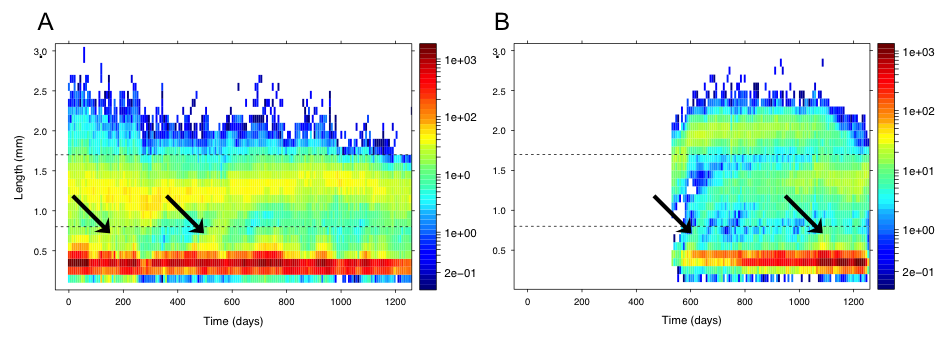
\includegraphics[width=0.95\textwidth]{3-1_ChapExp1/Fig/AnnSP1}
\caption[\lofimage{3-1_ChapExp1/Fig/AnnSP1}Examples of a population's
structure]{Examples of a population's structure - time diagram. A clone TO
replicate r3. B clone HA replicate 15. Dashed lines show the arbitrary
distinction made between juveniles ($<0.8$ mm), small adults ($<1.7$ mm) and
large adults ($>1.7$ mm) on the basis of all the structure time diagrams. Black
arrows mark some of the recruitment periods.}
\label{fig:AnSP1}
\end{center}
\end{figure}

\subsubsection{Size structure dynamics}

 We then look at the size structure dynamics, focusing on short-term events.
Figure \ref{fig:AnSP1}A and B show that although the size structure is rather
stable over time, dynamical processes can be observed on the structure-time
diagrams.

\paragraph{Cohort recruitment}

In Figure \ref{fig:AnSP1}A for instance, we can observe the recruitments of a cohort of
juveniles from the small sizes to the adult class. Such recruitment is very
clear between days 450 and 650, and less clear but nevertheless present around
day 200 (black arrows on the diagram). This shows that recruitment in the adult
class happens in waves. This dynamical pattern can be observed in every
population we followed, although it is not always very clear.

Figure \ref{fig:AnSP1}B also shows recruitment period, for instance at 600 days, but this
recruitment only goes up to the first class of adult. This observation on the
study case is also valid for every HA population with two separates classes of
adults. When two classes of adults are coexisting in a single population, we
never observe any clear period of recruitment from the first class to the bigger
class of adults (see appendices, populations r5, r7, r9, and 11 to 16).

Further more, these recruitment periods are very irregular. Indeed, they can
happen in a relatively short window of time, as in Figure \ref{fig:AnSP1}A, when the two
periods of recruitment are separated by only 200 days. But we also observe very
long periods without any recruitment. On the same figure, the second wave of
recruitment is followed by 500 to 600 days without clear recruitment wave to the
adult class. On the other hand, in certain conditions, recruitment can occur in
a rather regular cycle as for clone TO in population r7 where we can observe a
recruitment wave almost every 100 days.

These periods of recruitment offer a way to measure cohort growth rates by
estimating the slope of the cohort during the recruitment period. The example of
Figure \ref{fig:AnSP1}A between days 500 and 600 gives for the cohort a growth rate estimated
at $5.0\cdot 10^{-3}$ mm$/$d, that is to say 200 days to grow 1mm. This method
can be applied to any structure-time diagram where recruitment periods are distinctly
recognizable. In conditions of populations with sometimes very high densities
where tracking individuals is impossible, such a measure gives an insight into
populations life history traits and trajectories that would else be difficult to
obtain.

\begin{figure}[!ht]
\begin{center}
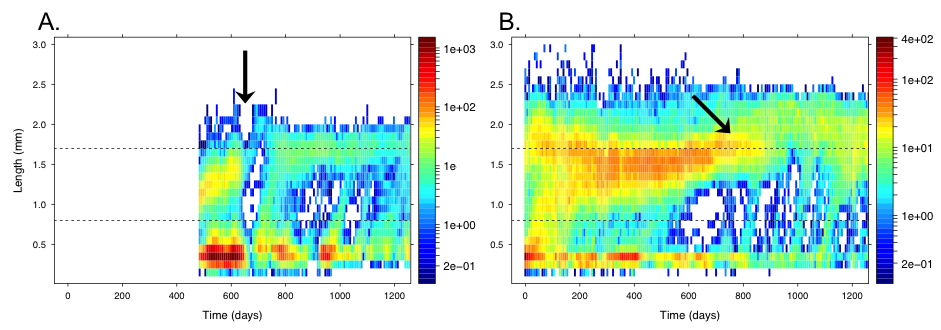
\includegraphics[width=0.95\textwidth]{3-1_ChapExp1/Fig/AnnSP2}
\caption[\lofimage{3-1_ChapExp1/Fig/AnnSP2}Examples of a population's
structure]{Example of a population where a catastrophic event (A, Clone TO
population 11, black arrow) or the senescence of the adult class (B, clone HA
population r4, black arrow) leads to growth of adults and recruitment of cohorts
of juveniles.}
\label{fig:AnSP2}
\end{center}
\end{figure}

Finally, recruitment periods sometimes follow catastrophic events, particularly
in clone TO. Figure \ref{fig:AnSP2}A shows an example of such a catastrophic
event (arrow).
We can observe that at day 670, almost all the population goes extinct except for
few adults. These adults immediately start growing rapidly to reach unusually
large size for clone TO, while a clutch hatches, immediately followed by the
recruitment of a cohort to the adult class. Several other populations of clone
TO present the same kind of catastrophic event followed by growth of remaining
adults and recruitment of a cohort: r6, r8, 12, 13.

Catastrophic events are not the only event that can cause cohort recruitments.
Indeed, the recruitment of a new cohort of juveniles can follow the decline of
the class of adults, as for population HA r4 (Figure \ref{fig:AnSP2}B arrow). Indeed, we can
see that a large number of adults recruits early in the dynamics, up to day 200,
but then remains stable for almost 600 days without recruitment. During this
long period, no recruitment is observed and the cohort of adults is slowly
decreasing in number of individuals with the old individuals dying. Around day
800, the number of adult left is very low, and we observe the recruitment of a
new cohort along with the growth of the remaining adults. This shows that the
aging of the adults can be a driver of the dynamics of the entire population.

\paragraph{Adult size plasticity}

As previously mentioned, we also observe adjustments of the adult body length
during the different dynamic events described. First, we can note that depending
on the demographic context, the adult cohorts stabilize at different body
lengths. The four populations shown as example (Figure \ref{fig:AnSP1} and
Figure \ref{fig:AnSP2}) have four different equilibrium size for the adult
class. The populations of clone TO stabilize between 1 and 1.5mm (Figure
\ref{fig:AnSP1}A) at high density (up to 100 adults and more than 1000
individuals in total) and 1.7mm (Figure \ref{fig:AnSP2}A) at a lower density
($\sim 200$ individuals and about 25 adults), whereas clone HA tends to be
bigger with adults in two classes around 1.5 mm and 2 mm in population 15
(Figure \ref{fig:AnSP1}B) with a population density around 800 to 1000
individuals, around 150 intermediate adults and 50 large ones, and in a single class around 1.7 mm (with
variations up to 2.2 mm) in population r4 (Figure \ref{fig:AnSP2}B) with only few hundred
individuals and few adults ($\sim 50$).

Moreover, adults can rapidly adjust their body length after stabilization in
case of dynamic events that change the population size structure. In the one
hand, in case of the catastrophes described previously, we observed that along
with a recruitment of a new cohort of juveniles, a catastrophic event is often
followed by a resumption of growth of the remaining adults up to $40\%$ of their
current size (Figure \ref{fig:AnSP2}A, adults grow from 1.5 mm up to 2.1 mm).
The same happens if the number of adults decreases due to background mortality
without any recruitment, as in Figure \ref{fig:AnSP2}B around day 800, with the
remaining adults growing from 1.7 mm up to 2.2 mm.

In the other hand, adults also seem to have the possibility to shrink in case
the number of adults quickly increases, for example when a large cohort of
juveniles recruits at the same time. Figure \ref{fig:AnSP2}B shows such a
phenomenon. Indeed, we can see that from day 0 to day 200, the average body
length of the group of adults above 1.5 mm decreases while a large cohort of
juveniles starts growing.
Between days 100 and 200, the size structure is tri-modal, but the large adults
continue to shrink until both classes of adults merge into one big group with a
bigger variability in adult body length. Such shrinking of the adults can be
observed in other population while a cohort recruits, for example in population
HA r1 to r3 and TO r5 and r9.

A summary of the different phenomena described here and the populations and
dates at which they have been observed is given in Table \ref{tab:AnSP1}.

{\tiny
\begin{longtable}{
	p{\dimexpr.12\linewidth-2\tabcolsep-1.3333\arrayrulewidth}% column 1
 	p{\dimexpr.128\linewidth-2\tabcolsep-1.3333\arrayrulewidth}
 	p{\dimexpr.128\linewidth-2\tabcolsep-1.3333\arrayrulewidth}% column 1
 	p{\dimexpr.128\linewidth-2\tabcolsep-1.3333\arrayrulewidth}
 	p{\dimexpr.12\linewidth-2\tabcolsep-1.3333\arrayrulewidth}% column 1
 	p{\dimexpr.12\linewidth-2\tabcolsep-1.3333\arrayrulewidth}
 	p{\dimexpr.126\linewidth-2\tabcolsep-1.3333\arrayrulewidth}% column 1
 	p{\dimexpr.126\linewidth-2\tabcolsep-1.3333\arrayrulewidth}}
 	
\caption{Summary of the state and dynamic observations. The numbers in the table
are the dates or the intervals where to see the event
described.}\label{tab:AnSP1}\\
 	\hline
 	\endhead
 	
\hline
\endfoot

Populations & Trimodal & Long period without recruitment & Frequent recruitment
& Catastrophic event & Adult cohort aging & Adult growing to adjust & Adult
shrinking to adjust\\
\hline\\
HA r1 & - 			& - 		& - 		& - 	& 500  & 500-650  & 650-750  \\
HA r2 & - 			& - 		& - 		& - 	& 800  & 650-900  & - 		 \\
HA r3 & - 			& - 		& - 		& - 	& 800  & 900-1000 & 1000-1250\\
HA r4 & - 			& - 		& - 		& - 	& 800  & 600-1000 & -        \\
HA r5 & 600-1000 	& - 		& - 		& - 	& 1000 & - 		  & - \\
HA r6 & - 			& 800-1250 	& - 		& - 	& -    & - 		  & - \\
HA r7 & 700-1100 	& - 		& - 		& - 	& 1000 & - 		  & - \\
HA r8 & 600-1000 	& - 		& - 		& - 	& 950  & - 		  & - \\
HA r9 & 700-1200 	& 700-1100 	& - 		& - 	& -    & - 		  & - \\
HA 10 & 600-900 	& - 		& - 		& - 	& 900  & - 		  & - \\
HA 11 & 600-1100 	& 700-1250 	& - 		& - 	& 1100 & - 		  & - \\
HA 12 & 600-900 	& - 		& 600-1250 	& - 	& 1000 & - 		  & - \\
HA 13 & 600-1100 	& - 		& 600-1250 	& - 	& 1100 & - 		  & - \\
HA 14 & 600-1100 	& 600-1000 	& - 		& - 	& 1100 & - 		  & - \\
HA 15 & 600-1100 	& - 		& 600-1250 	& - 	& 1100 & - 		  & - \\
HA 16 & 600-1200 	& - 		& - 		& - 	& 1200 & - 		  & - \\
TO r1 & - 			& 400-600 	& 0-400 	& - 	& 400  & 400-600  & -\\
	  &				& 700-1000	& 1000-1250 & 		&	   &		  &\\
TO r2 & - 			& 500-750 	& 0-450 	& - 	& 400  & 500-700  & - \\
	  & 			& 			& 1000-1250 &		&	   &		  &\\
TO r3 & - 			& 600-1250 	& - 		& - 	& -    & - 		  & 0-200\\
TO r4 & - 			& - 		& 0-1250	& - 	& 400  & - 		  & 700-1000\\
TO r5 & - 			& - 		& - 		& 900 	& -    & 900-1000 & 500-700\\
TO r6 & - 			& 600-950 	& - 		& 950 	& -    & 950-1000 & -\\
TO r7 & - 			& - 		& 500-1250 	& - 	& -    & - 		  & -\\
TO r8 & - 			& 600-800 	& 800-1250 	& - 	& 1000 & 1000-1100& -\\
TO r9 & - 			& 600-1000 	& - 		& - 	& 950  & 900-1000 & 500-600\\
TO 11 & - 			& - 		& 700-1250 	& 650 	& -    & 650-750  & -\\
TO 12 & - 			& - 		& - 		& 750 	& -    & 750-850  & -\\
TO 13 & - 			& 500-800 	& 800-1250 	& 800 	& -    & - 		  & -\\

\end{longtable}
}

\subsection{Quantitative analysis of populations dynamics}

We use here a quantitative approach based on the principle component analysis to
simplify our complex dataset into few dimensions, making it easier to comprehend
and manipulate, and to allow for a more thorough statistical analysis of the
dependency of the size structure and its dynamics on diverse factors such as the
genetic lineage or the state itself.

\subsubsection{Principal components}

As described in the methods we decompose our compiled dataset of all our
populations into principal components, without accounting for time dependence.
We use 30 size classes in our dataset going from 0 to 3 mm by steps of 0.1 mm.

\begin{figure}[!ht]
\begin{center}
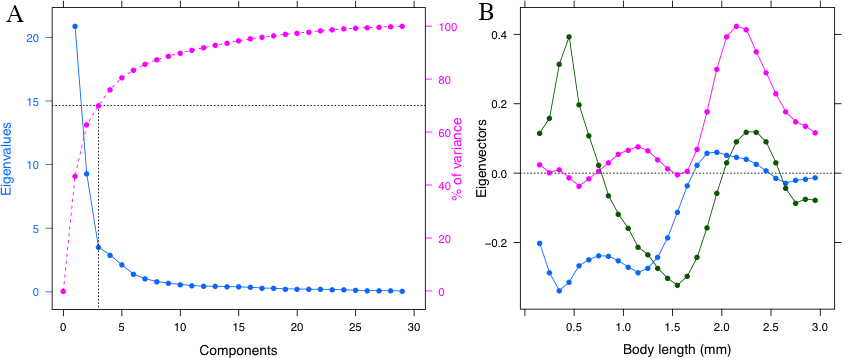
\includegraphics[width=0.95\textwidth]{3-1_ChapExp1/Fig/AnnSP3}
\caption[\lofimage{3-1_ChapExp1/Fig/AnnSP3}Scree plot of the PCA and
coordinates of first components]{A. Scree plot of the principal component
analysis.
The plain line gives the eigenvalues whereas the dashed line is the cumulative percentage of variance explained. B. Coordinates of the size classes on the first three eigen
vectors.}
\label{fig:AnSP3}
\end{center}
\end{figure}

Figure \ref{fig:AnSP3} shows the cumulative percentage of the variance explained
by the components along with the scree plot of the principal component analysis.
Looking at the eigenvalues, we can see a clear break in the slope after the
first three components. This suggests that keeping only the first three
components to simplify the data is sufficient to explain correctly the different
patterns in size distribution observed in our data. These first three components
represent together $70\%$ of the total variance of our data.

Figure \ref{fig:AnSP3}B shows the coordinates of the original vectors of our data set, that is
to say the size classes, on the first three eigenvectors. This allows seeing
what part of the original distribution is explained by each of the eigenvectors.
We can see that the first components, which explains by itself $43\%$ of the
variance, represents essentially the first half of the size classes, with
individuals smaller than 1.6mm. On the contrary, the second component that
explains $20\%$ of the variance represents both the small adults (0.8 to 1.3 mm)
and individuals bigger than 1.6mm with a major part explained by the larger
ones. Finally, the third component ($7\%$ of the variance) allows
distinguishing between a group of intermediate individuals with a size between 0.8 and 1.9mm,
and the very small individuals (<0.8 mm) and very large individuals (>1.9 mm).

Altogether, the first three principal components of our decomposition give a
good description of the majority of the information present in our data, by
decomposing the size classes into several groups of interest: (i) the juveniles
(<0.6mm), negative on the first axis and positive on the third one, (ii) small
adults (between 0.6 mm and 1.2mm), negative on the first and the third axes and
positive on the second one, (iii) intermediate adults (1.2 mm to 1.9 mm) mostly
negative on the third axis, and (iv) big adults (>1.9 mm) positive on the second
axis. Those four groups describe well the groups identified using the
structure-time diagrams, but without deciding for size classes a priori,
justifying a simplification of our data into four size classes. The number of
individuals in each class gives an idea of the overall size distribution.

As the first two components bare most of the variance ($63\%$), we reduced even
more the data by dropping the third component, keeping only the first two in the
rest of the analysis. This allows a 2D-representation of the structured data on
a phase plane with the two components as axes, with the original vectors
superimposed (biplot). Figure \ref{fig:AnSP4} shows the biplot with a
color-coding of the four major size classes previously described. The third class, the intermediate
adults, has been coded in two different colors depending whether individuals are
bigger or smaller than 1.65 mm, showing that presence of the former will cause a
decrease along the first axis whereas the latter will cause an increase along
the second axis. First, we can see in a different way what have been discussed
with Figure \ref{fig:AnSP3}, that is to say, that the first component represents mostly the
smaller individuals whereas the second one represents the bigger one. But we
observe as well that the data plotted on the first two components spread in four
distinct clusters, indicating four significantly distinct types of size
structures in our dataset.

\begin{figure}[!ht]
\begin{center}
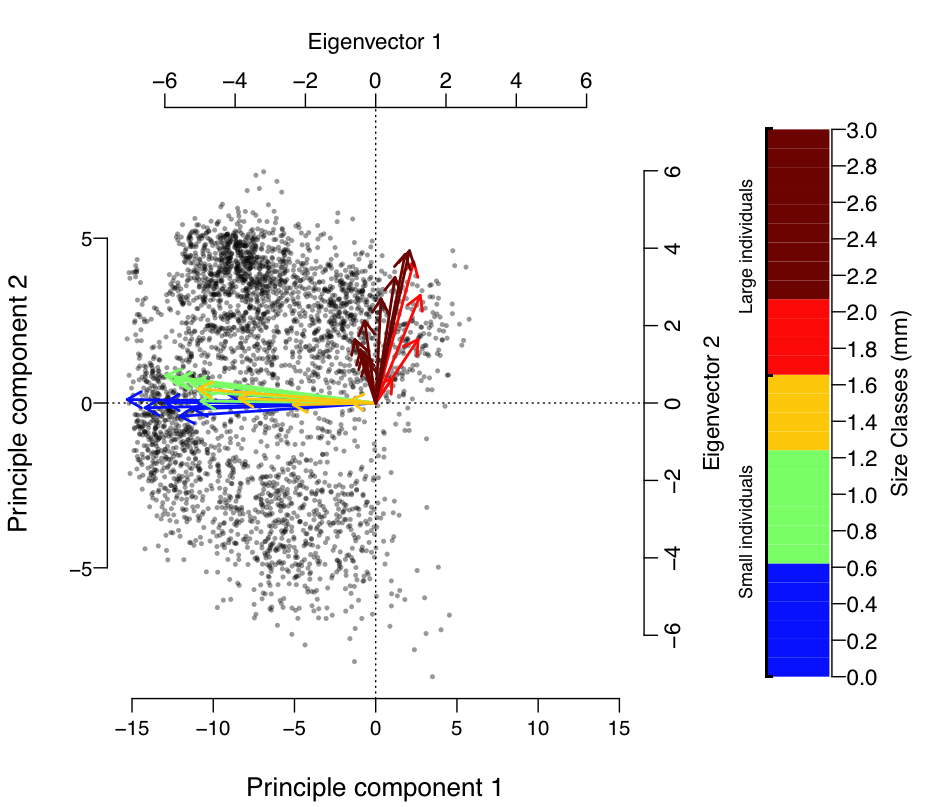
\includegraphics[width=0.95\textwidth]{3-1_ChapExp1/Fig/AnnSP4}
\caption[\lofimage{3-1_ChapExp1/Fig/AnnSP4}Biplot of the principle component
analysis]{Biplot of the principle component analysis with the first two
components. The black dots are the data represented on the first two principle
components (primary x and y axes). The arrows are the original
size classes projected on the first two eigenvectors (secondary x and y axes).
The color-coding represents the four groups previously identified.}
\label{fig:AnSP4}
\end{center}
\end{figure}

\subsubsection{Four groups of size structure}

We hence used a non-hierarchical clustering method to identify four groups in
the original dataset using the k-means algorithm. Figure \ref{fig:AnSP5} shows the projection
of the four groups on the first two components. We can see that the clustering
analysis conducted on the entire dataset groups well together the four groups
that were visible on Figure \ref{fig:AnSP4}. We plotted together on four structure-time
diagrams the observations from each of the groups to verify the interpretation
of each group in terms of distribution of adults (see supplementary materials).

\begin{figure}[!ht]
\begin{center}
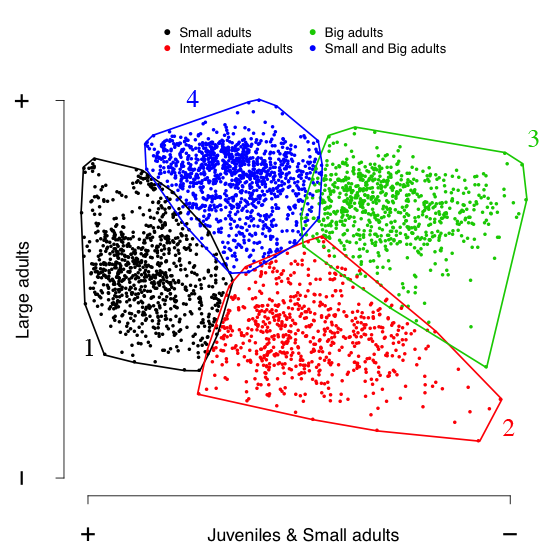
\includegraphics[width=0.95\textwidth]{3-1_ChapExp1/Fig/AnnSP5}
\caption[\lofimage{3-1_ChapExp1/Fig/AnnSP5}Results of the clustering analysis
with four groups]{Results of the clustering analysis with four groups. The
colors give the interpretation of the groups in terms classes of adults present. The lines show the spatial domain in the (PC1, PC2) space, this domain is then reported in
the trajectories for each population (supplementary materials). For convenience,
the regions are numbered from 1 to 4 as reported on the plot.}
\label{fig:AnSP5}
\end{center}
\end{figure}

This representation on the (PC1, PC2) phase plan now gives a quantitative tool
to determine the general structure of a population at a given time, and by
looking at the trajectory in the phase plan over time, a way to analyze the
dynamics across the different characteristic structures.

\subsubsection{2D representations of the previous examples}

\begin{figure}[!ht]
\begin{center}
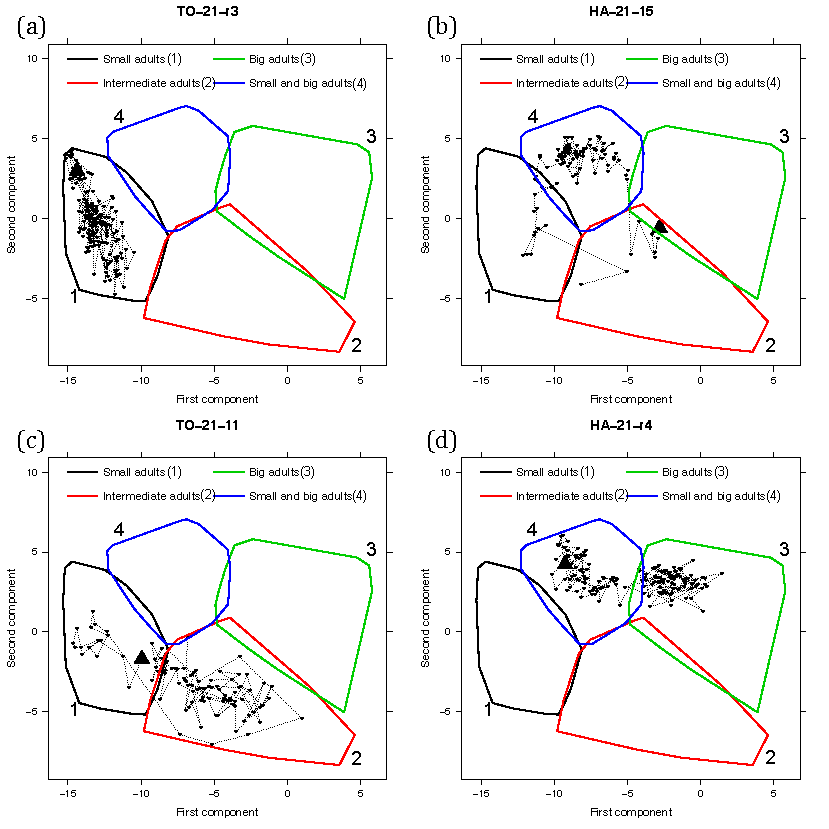
\includegraphics[width=0.95\textwidth]{3-1_ChapExp1/Fig/AnnSP6}
\caption[\lofimage{3-1_ChapExp1/Fig/AnnSP6}Time trajectories in the first two principle components]{Time trajectories in the first two principle components.
Colored lines mark the previously identified regions. The triangles mark the
starting points of the four time series. The points are the population
observations. The dotted lines are link the points in time.}
\label{fig:AnSP6}
\end{center}
\end{figure}

Figure \ref{fig:AnSP6} shows the same time series as Figure \ref{fig:AnSP1} (A
and B) and Figure \ref{fig:AnSP2} (C and D), but represented as trajectories in
the main principal components phase plan.

On the one hand, we now have a numerical evidence that shows that population r3
of clone TO spends all its time with a structure composed of juveniles and small
adults, whereas population 11 starts with small adults, but then shifts to a
structure with less juveniles, and intermediate adults. On the other hand, both
populations of clone HA exhibit structures with both small and large adults.
Population 15 starts with a growth period with intermediate adults reaching
large sizes, followed by a long period with both small and large adults, meaning
that new individuals reached adulthood but stayed small. Finally, large adults
died out, driving the trajectory to the small adults region, and finishing with
small adults growing to intermediate adults. The last population always has
large adults. The first part also has small adults that grow into large ones,
shifting the population from the blue to the green region.

\subsubsection{Stability and state transitions in our size structured
population dynamics}

This representation of the time trajectory in a space of the first two principle
components allows determining a date for the transitions from one state to
another, along with a residence time in a given state.

\begin{figure}[!ht]
\begin{center}
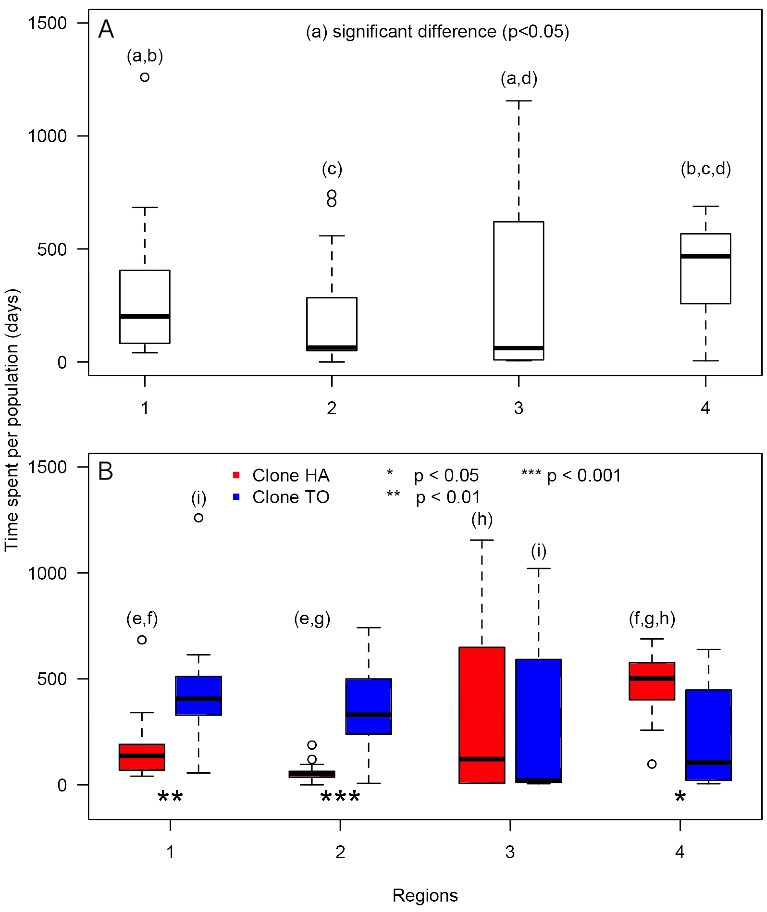
\includegraphics[width=0.85\textwidth]{3-1_ChapExp1/Fig/AnnSP7}
\caption[\lofimage{3-1_ChapExp1/Fig/AnnSP7}Time spent in each stable size
distribution region]{Time spent in each stable size distribution region in days
for the two clones merged (A) and separated (B). The letters denote a
significant difference between the corresponding distributions (Tests:
two-sample Kolmogorov-Smirnov test, A: (a) D=0.5, p=0.01, (b) D=0.38, p=0.05,
(c) D=0.51, p=0.002, (d) D=0.43, p=0.03 B: (e) D=0.54, p=0.02, (f) D=0.78,
p=0.0003, (g) D=0.93, p=3x10-6, (h) D=0.53, p=0.03, (i) D=0.67, p=0.04).}
\label{fig:AnSP7}
\end{center}
\end{figure}

Figure \ref{fig:AnSP6} shows four different types of trajectories with different residence
time in the different regions. On Figure \ref{fig:AnSP6}A for instance, we can see that the
population’s structure is very stable and remains the entire 1200 days in the
same region characterizing a structure with juveniles and small adults. In
contrast, Figure \ref{fig:AnSP6}B, C and D show transitions between different regions. More
precisely, population HA 15 (Figure \ref{fig:AnSP6}B) starts in the region with intermediate
adults (red) where it spends about 50 days until it reaches a temporary
equilibrium in the region with both small and big adults for about 550 days,
before going back to the region with intermediate adults. Using the trajectory
in the decomposed space, we can date the first transition at day 57 and the
second one at day 608.

The same analysis can be conducted on each of our 28 populations. First, we look
at the time spent in each region (1 to 4) by each population, corresponding to
the time spent in each of the stable size distributions identified. Figure
\ref{fig:AnSP7}A shows that region 2 is the least stable region with the
smallest amount of time spent in it. This region corresponds to a size distribution with juveniles and
intermediate adults. This region can be seen as a region of transition that is
crossed when going to one of the other stable structures. In contrast, region 4
with a tri-modal distribution is very stable. This is due to the presence of a
cohort of large adults that have a long survival and suffer a low level of
competition, stabilizing the structure. Although the variability is very high in
region 3, the maximums of time spent are in this region, with the same
stabilizing effect of very large individuals. Region 1 is also quite stable and
corresponds to structures where the density is very high causing a big
resilience of the size structure, explaining the relatively long residence time
in it.

Figure \ref{fig:AnSP7}B shows the times of residence in the different regions separated by
clones. We can see in this figure that the patterns of region occupation are
very different depending on the clones. In more details, clone TO spends most of
its time in region 1 and 2 where adults have a small to intermediate body
length, and a very small amount of time with large adults or in a tri-modal
state. Indeed, clone TO is generally smaller than clone HA, and the occurrences
of a type 3 and 4 structure are either due to exceptional conditions followed by
a transition to a type 1 or 2 size structure. On the contrary, clone HA spends
significantly more time in region 3 and 4 than 1 and 2. This confirms the
observations from the qualitative analysis showing that a lot of HA population
exhibited structures with large adults and long lasting tri-modal distribution.
More over this allows us to use the structure type (1 to 4) as a simple rule of
thumb to discriminate between the clones, type 1 and 2 being characteristic
structures of clone TO whereas type 3 and 4 are characteristic of clone HA.


\begin{table}
\small
\centering
\caption{\label{tab:AnSP2}Number of transitions observed in the 28 populations between the different regions. In parenthesis, decomposed between clones HA and TO.}
\renewcommand{\arraystretch}{1.5}% Wider
\begin{tabular}{|rr|cccc|}
\hline 
	&  & & \multicolumn{2}{c}{Region of arrival}  & \\	
	&	& 1 & 2 & 3 & 4 \\
\hline
\parbox[t]{2mm}{\multirow{4}{*}{\rotatebox[origin=c]{90}{Region of origin}}} &
1 & - & 22 (HA: 2, TO: 20) & 0 & 24 (HA: 17, TO: 7) \\
 & 2 & 19 (HA: 4, TO: 15) & - & 26 (HA: 12, TO: 14) & 19 (HA: 8,
TO: 11)\\
 & 3 & 0 & 23 (HA: 10, TO: 13) & - & 32 (HA: 27, TO: 5) \\
 & 4 & 32 (HA: 23, TO: 9) & 17 (HA: 5, TO: 12) & 32 (HA: 26, TO: 6)
& -\\
	
\hline

\end{tabular} 
\end{table}

Table \ref{tab:AnSP2} shows the number of occurrences of each possible
transition between regions in all our time series. First, we can note that two transitions are
never observed. Indeed it is biologically not likely to go from region 1 (small
adults) directly into region 3 (large adults) without going through region 2,
and vice versa, but the number of occurrence of the other transitions is quite
homogeneous. Second, looking at the differences between HA and TO (in
parentheses), we can see that the frequency of each transition is no longer
homogeneous within a given clone. For instance, some of the transitions are very
frequent in clone HA but rare in clone TO (1 $\rightarrow$ 4, 3 $\rightarrow$ 4, 4 $\rightarrow$ 1 and 4 $\rightarrow$ 3), whereas
others are mainly due to clone TO (1 $\rightarrow$ 2, 2 $\rightarrow$ 1). This is due to an intrinsic
difference between the two clones and their life histories that result in
different attractors in term of stable size structures (region 3 and 4 in HA,
regions 1 and 2 in TO).

\section{Discussion}

We have described and quantitatively analysed detailed time series of the
structure of 28 populations of two different clonal lineages (16 populations of
clone HA, 12 of clone TO)

\subsection{Dynamic consequences of genetic differences}

We showed different patterns of size structure states and dynamics that were
observed numerous times in our different populations. Interestingly, the
patterns observed are different depending on the genetic background. The two
clones we studied here (HA and TO) are known for their different life history
strategies \autocites{tully2006a,tully2008a}. Indeed, whereas
clone HA has a low-flexibility strategy that produces small eggs and barely increases its
reproductive investment in response to the environmental amelioration, clone TO
has a high-flexibility strategy, characterized by larger egg size and highly
flexible reproductive investment \autocites{tully2008a}.

The different life history strategies also have consequences on the size
structure states and dynamics of each clone. Indeed, clone HA tends to favour
growth over reproduction, leading to structures with larger adults than clone
TO, which favours reproduction and generally has small adults. Further more, the
ability of clone HA to produce very large individuals explain its ability to
reach a structure of type 4 with a tri-modal distribution. Indeed, when the
conditions are favourable, very large individuals with high survival capacity
emerge in the population. Once settled, they dominate the population and prevent
other adults to reach their size, blocking them at a smaller body length,
causing the third mode in the size distribution to appear.

These consequences of the genetic background show how important it is to know
the life history of the species studied in order to understand the size
structure dynamics that can be observed, and to be able to predict their
possible outcome.

\subsection{The role of initial conditions}

Interestingly, although the type 4 structure seems highly stable, it only
appeared in our populations at the very beginning of the time series. Indeed,
this size structure is locally stable but depends a lot on the initial
conditions to be reached. For a population to reach a type 4 size structure, two
criteria need to be met: (i) the individuals in the population need to be able
to grow quickly and reach a long body size, which is the case of individuals
from clone HA but not TO; (ii) the level of competition needs to be at its
minimum, which translates in the absence of adults in the population and a small
density of juveniles. In these conditions, the juveniles will very quickly grow
to large body size, and impose their dominance on the rest of the population by
monopolizing the resources.

As for the type 4 size structure, the other observed structured are also
dependent on the initial conditions. An artificially high density of juveniles
as initial state will lead to a type 1 size structure whereas a relatively even
size distribution between juveniles, small and intermediate adults will
generally result in a type 2 size structure for clone TO and a type 3 for clone
HA.

The determinant role of initial conditions in the structure state reached by a
population illustrates the coexistence of the four quasi-stable attractors, even
though the breeding conditions are kept the same throughout time for all the
populations. Moreover, the transitions from two stable states are either caused
by the aging of the large adult cohort that disappear, or catastrophic events
that reset the population to new initial conditions and lead it to a new
attractor. Populations in which none of the above occurs remain in the same size
structure during the whole period of measurement, like population TO r3 (Figures
\ref{fig:AnSP1}A and \ref{fig:AnSP6}A) that stays in a type 1 structure during more than 1200
days.

This sensitivity to initial conditions also illustrates clearly the major
importance of including the structure of the population in the analysis of its
dynamics rather than the simple number of individuals. Indeed, with the same
number of individuals, starting a population with small individuals rather than
large ones will have a dramatic impact on the future dynamics of the whole
population, including its potential survival. This confirms previous results
shown by \textcites{benton2005a} on soil mite populations.

\subsection{The role of large individuals on the structure dynamics, an evidence
for interference competition}

Throughout our analyses, we have demonstrated the importance of large
individuals in the dynamics of the size structure of the population. The
resources need to be abundant and the competition for its access as low as
possible for an individual to reach a very large size. If the access to the
resources was only limited by exploitative competition, every individual would
gain access to part of the resource and the energy budget theory predicts that
large sizes are disadvantaged due to less efficient energy consumption compared
to smaller individuals \autocites{de-roos2003b}. In these conditions, the
size structure of the populations would inevitably tend to a structure where small individuals
dominate in number and have a size close to their size at maturation, and
emergence of large individuals would be impossible.

In our dynamics, we observed evidences for a more complex regulation system: (i)
in several conditions, large individuals can emerge and survive in the
population, (ii) in cases of catastrophic events, the disappearance of the
larger individuals is immediately followed by the recruitment of a new cohort,
(iii) the aging of cohorts of large adult and their progressive disappearance
also provoke new recruitment periods, and (iv) dense cohort of adults are often
concomitant with long periods without recruitment. These different observations
support a regulation system involving the dominance of the population by the
larger individuals that monopolize the resources, preventing access to the
smaller individuals that stay small. This mechanism can be seen as interference
competition. When the number of large individuals decreases, the competition
pressure put on the smaller ones is progressively released, until the small
individuals gain access to the resource, and along with the remaining large ones
can resume their growth.

Interference competition is believed to be widespread in nature and to play an
important role on populations dynamics. Our study shows that analysing the
temporal dynamics of the size structure of a population rather than its overall
dynamics allows to describe more precisely the mechanisms involved in its
regulation, such as the role of the life history strategies that the individuals
follow, the importance initial conditions and the type of intraspecific
interactions.

We believe that our study is a striking example of how a population dynamics can
be controlled by large individuals that monopolize the resources, giving rise to
different possible structures and complex dynamics that are highly dependent on
the life history of the individuals. Modelling interference competition in a
structured population would allow confirming that with a high enough intensity,
interference competition is sufficient to cause emergence and survival of large
individuals, and dynamics involving multimodal size distributions.

\newpage
\section{Supplementary materials}

\subsection{Structure-time diagrams and 2D time trajectories of each population
studied}

~
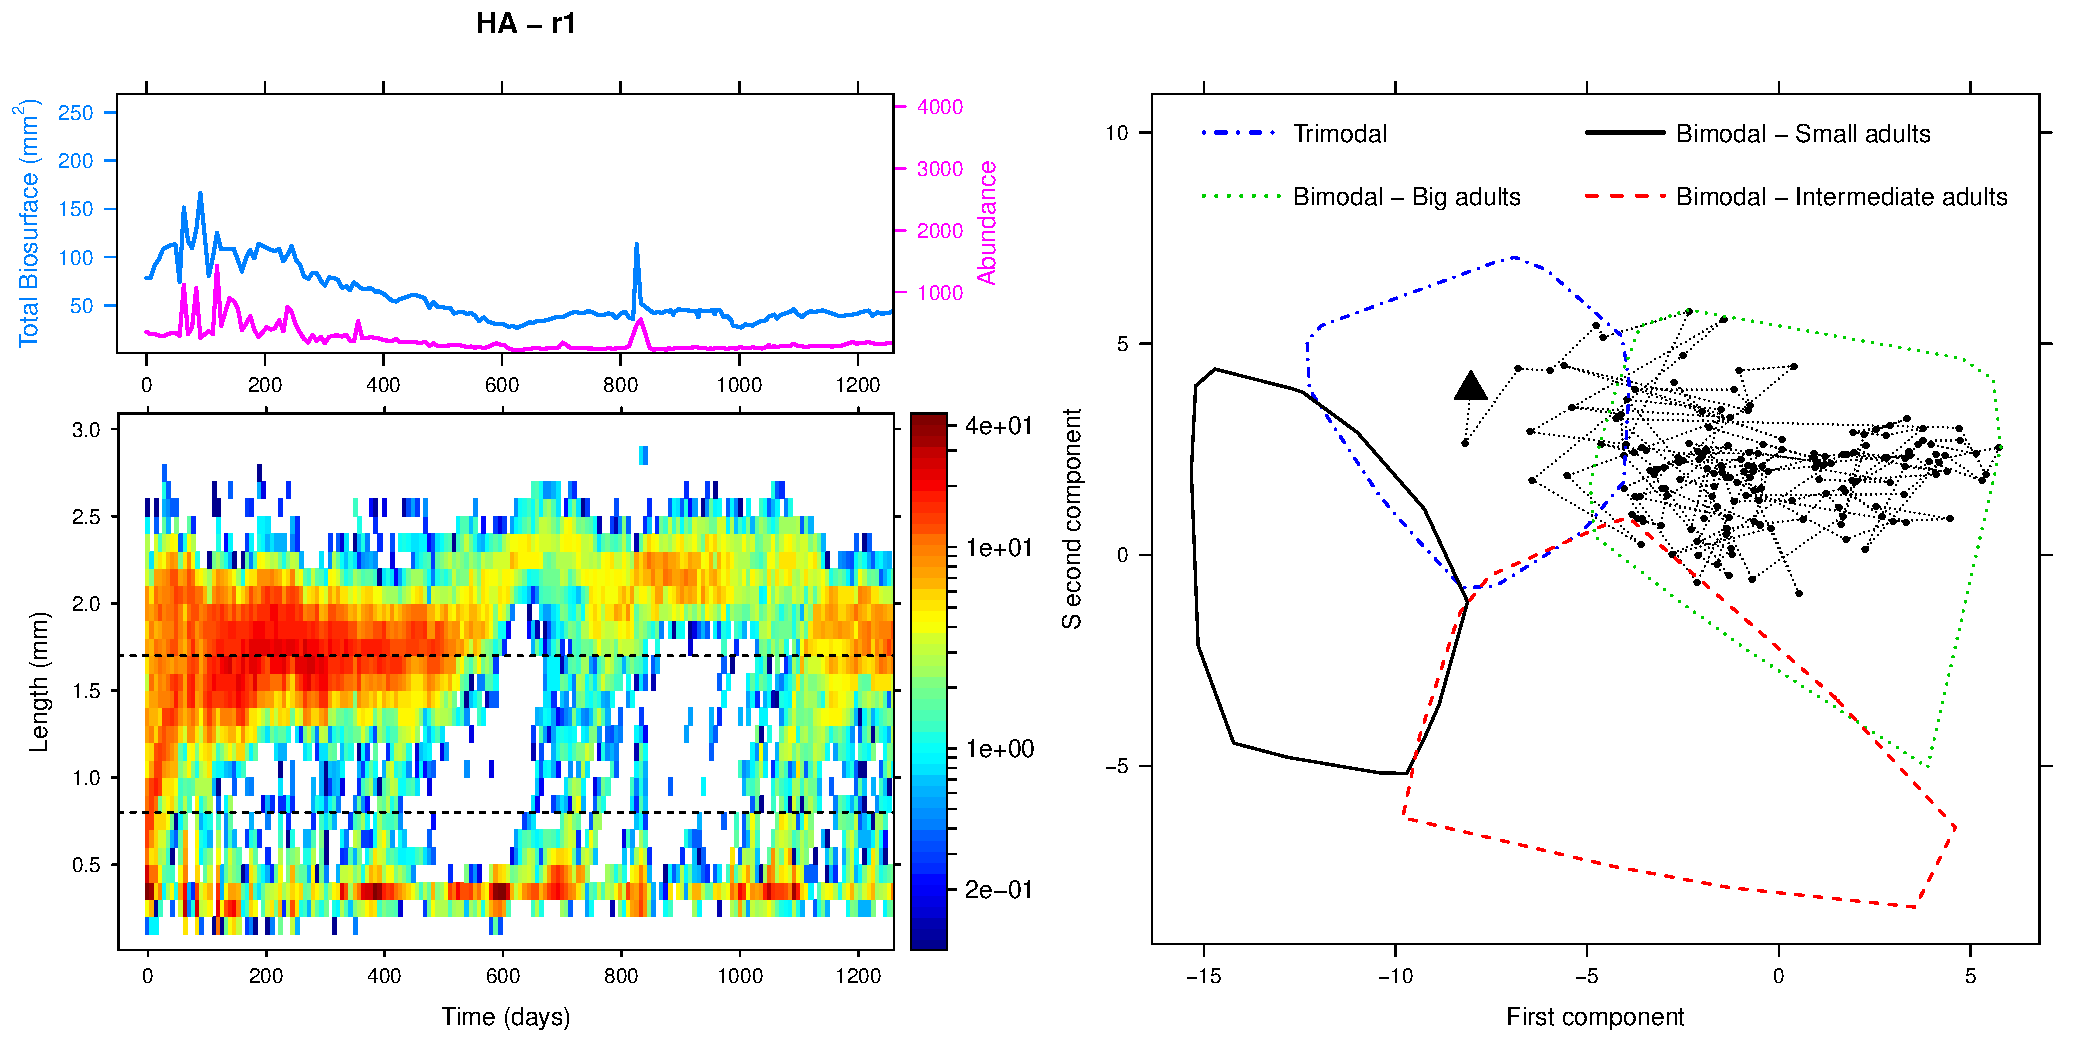
\includegraphics[height=0.33\textheight]{3-1_ChapExp1/Fig/HA-21-r1}

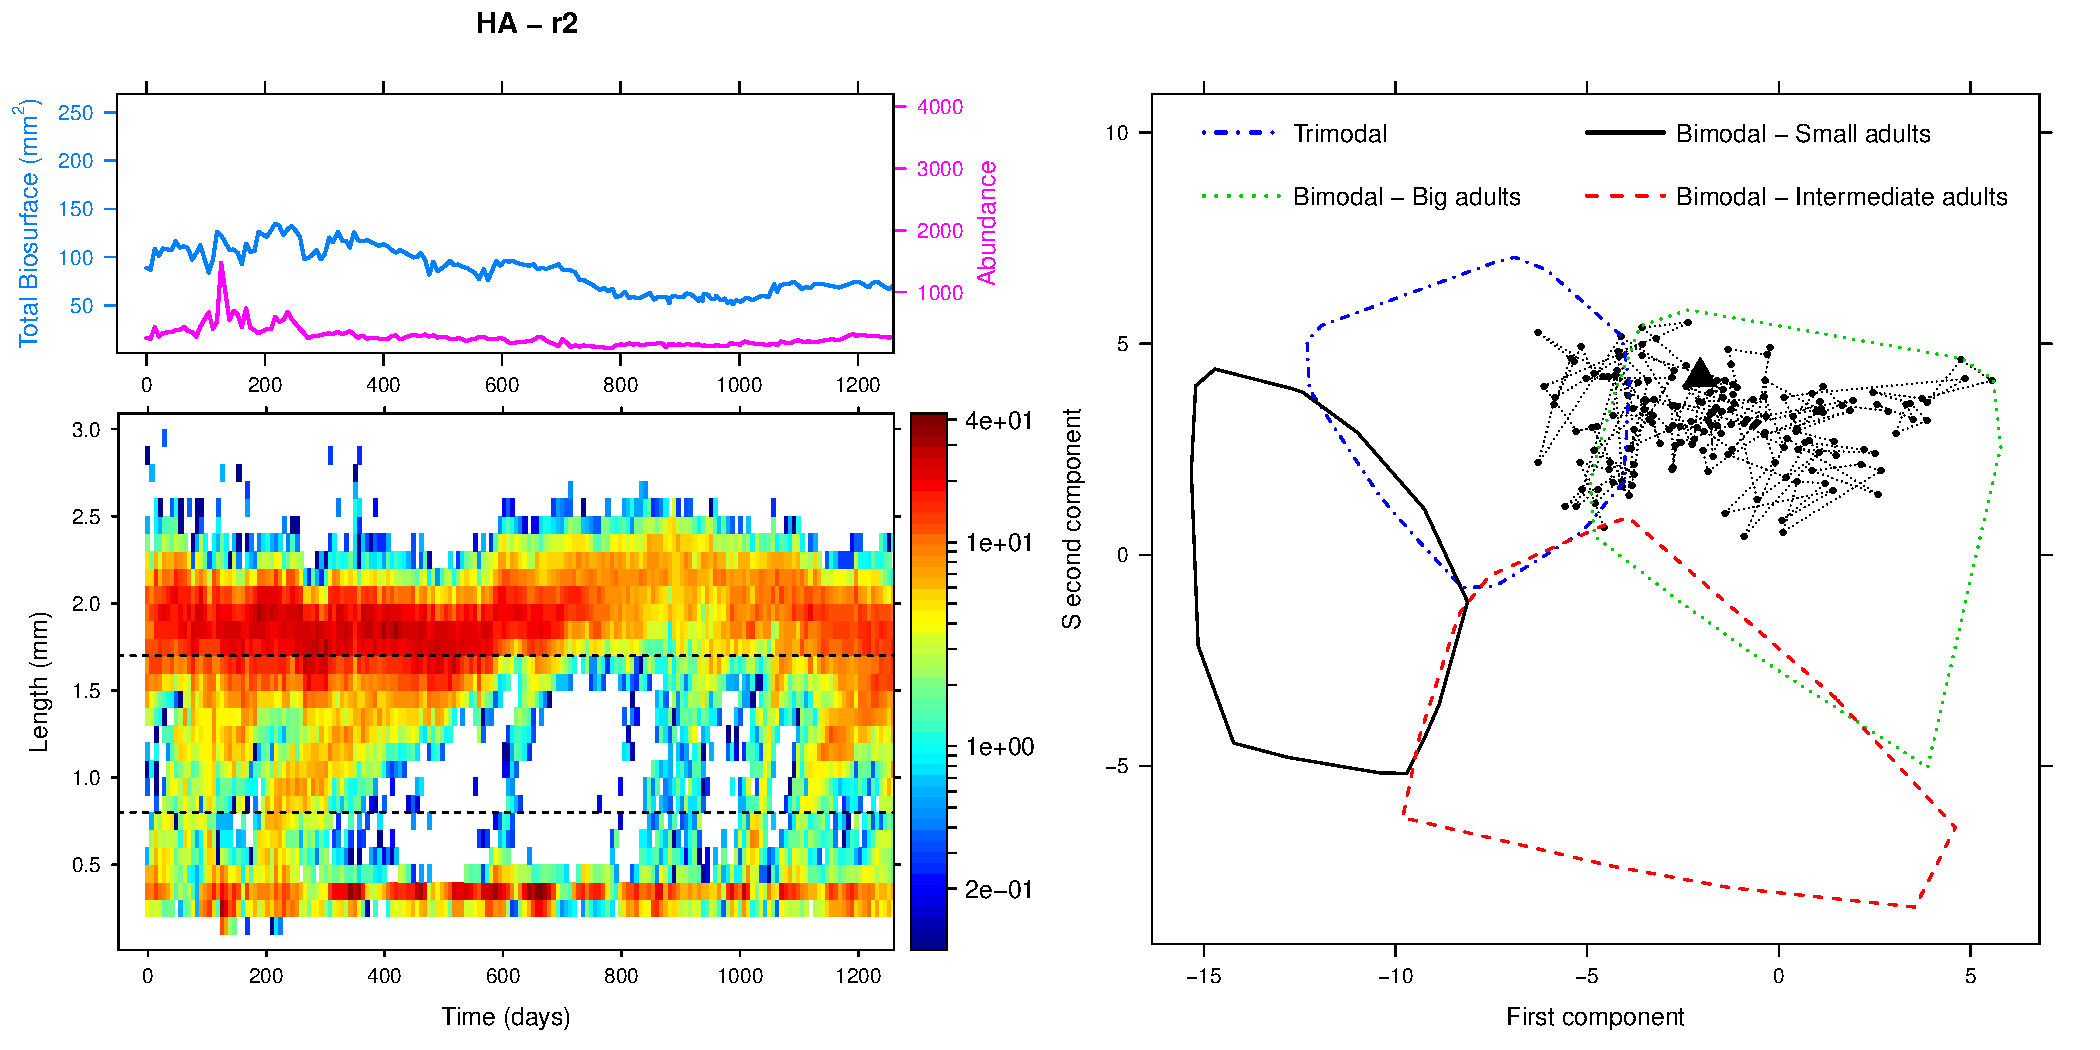
\includegraphics[height=0.33\textheight]{3-1_ChapExp1/Fig/HA-21-r2}

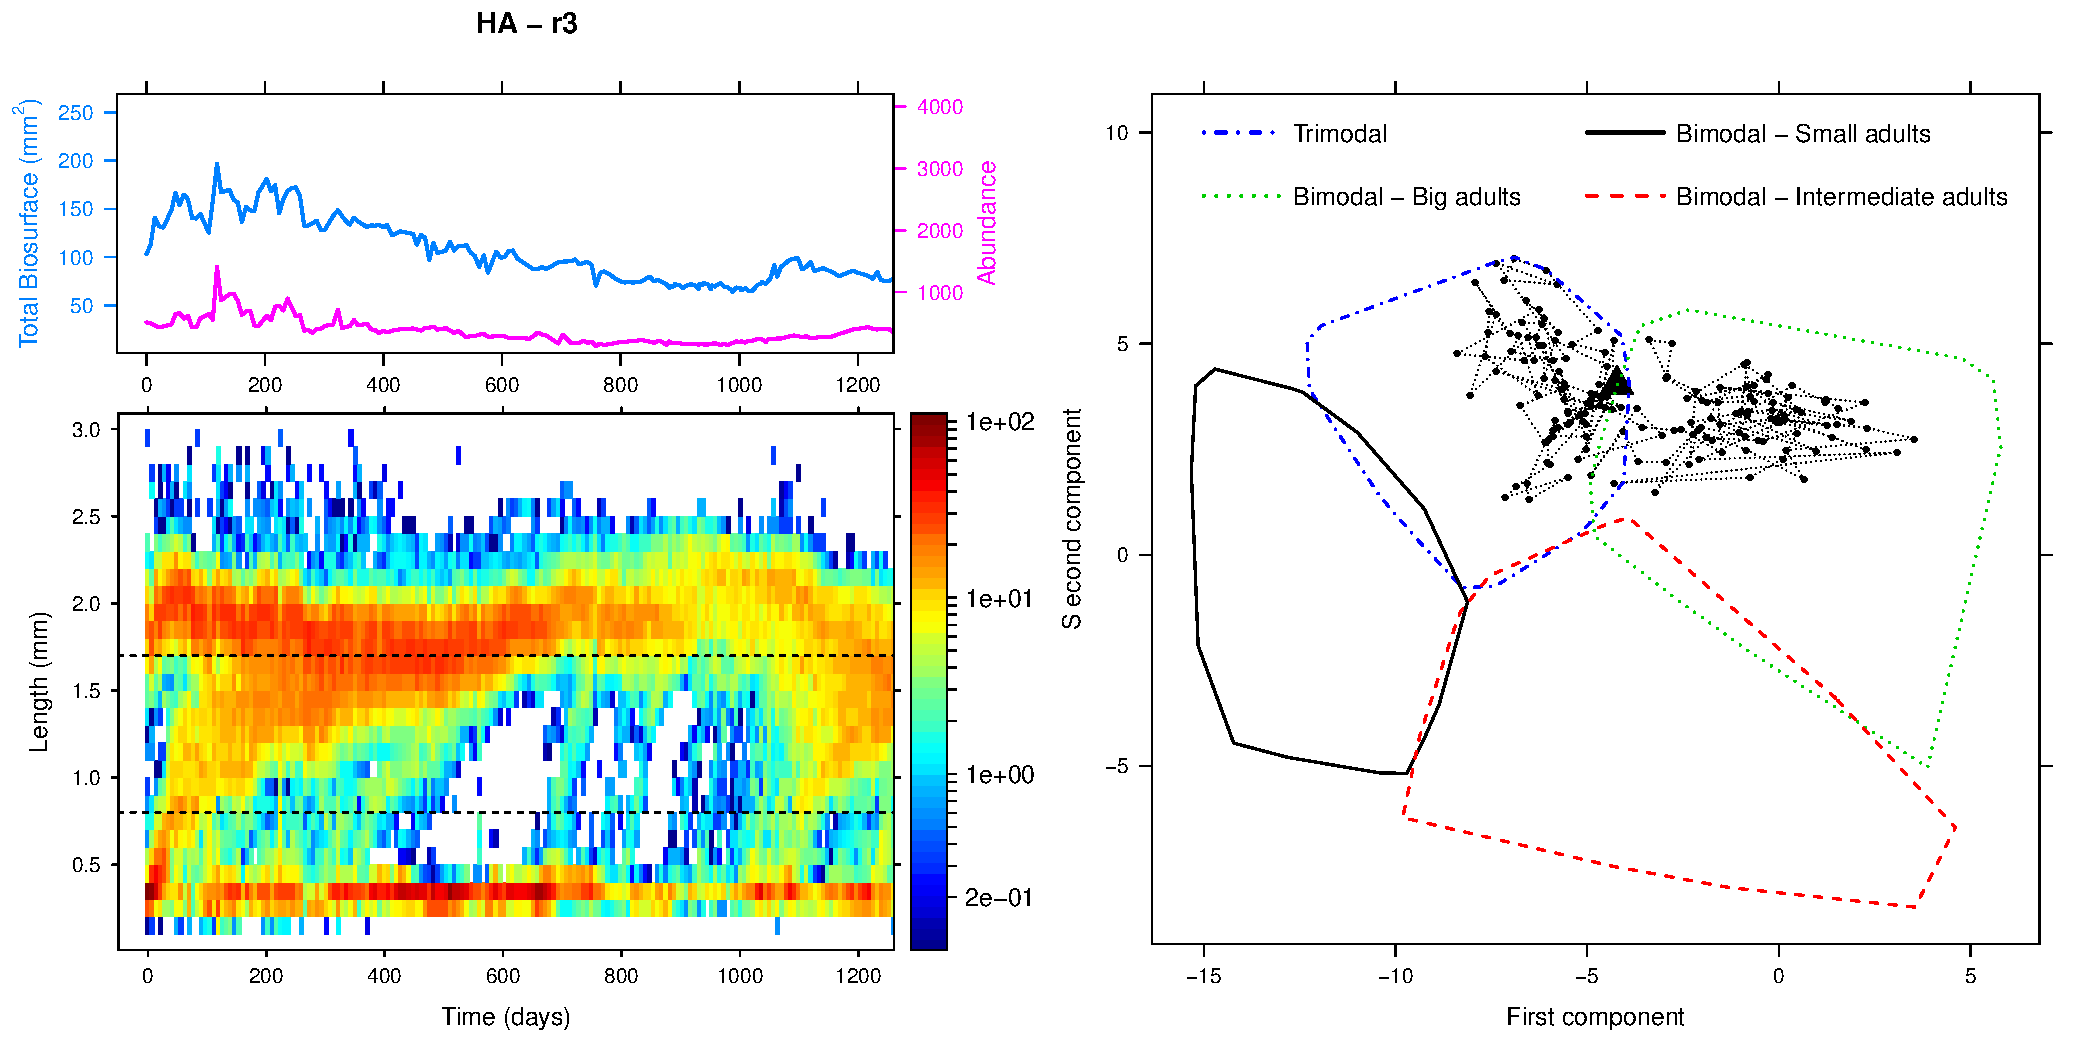
\includegraphics[height=0.33\textheight]{3-1_ChapExp1/Fig/HA-21-r3}

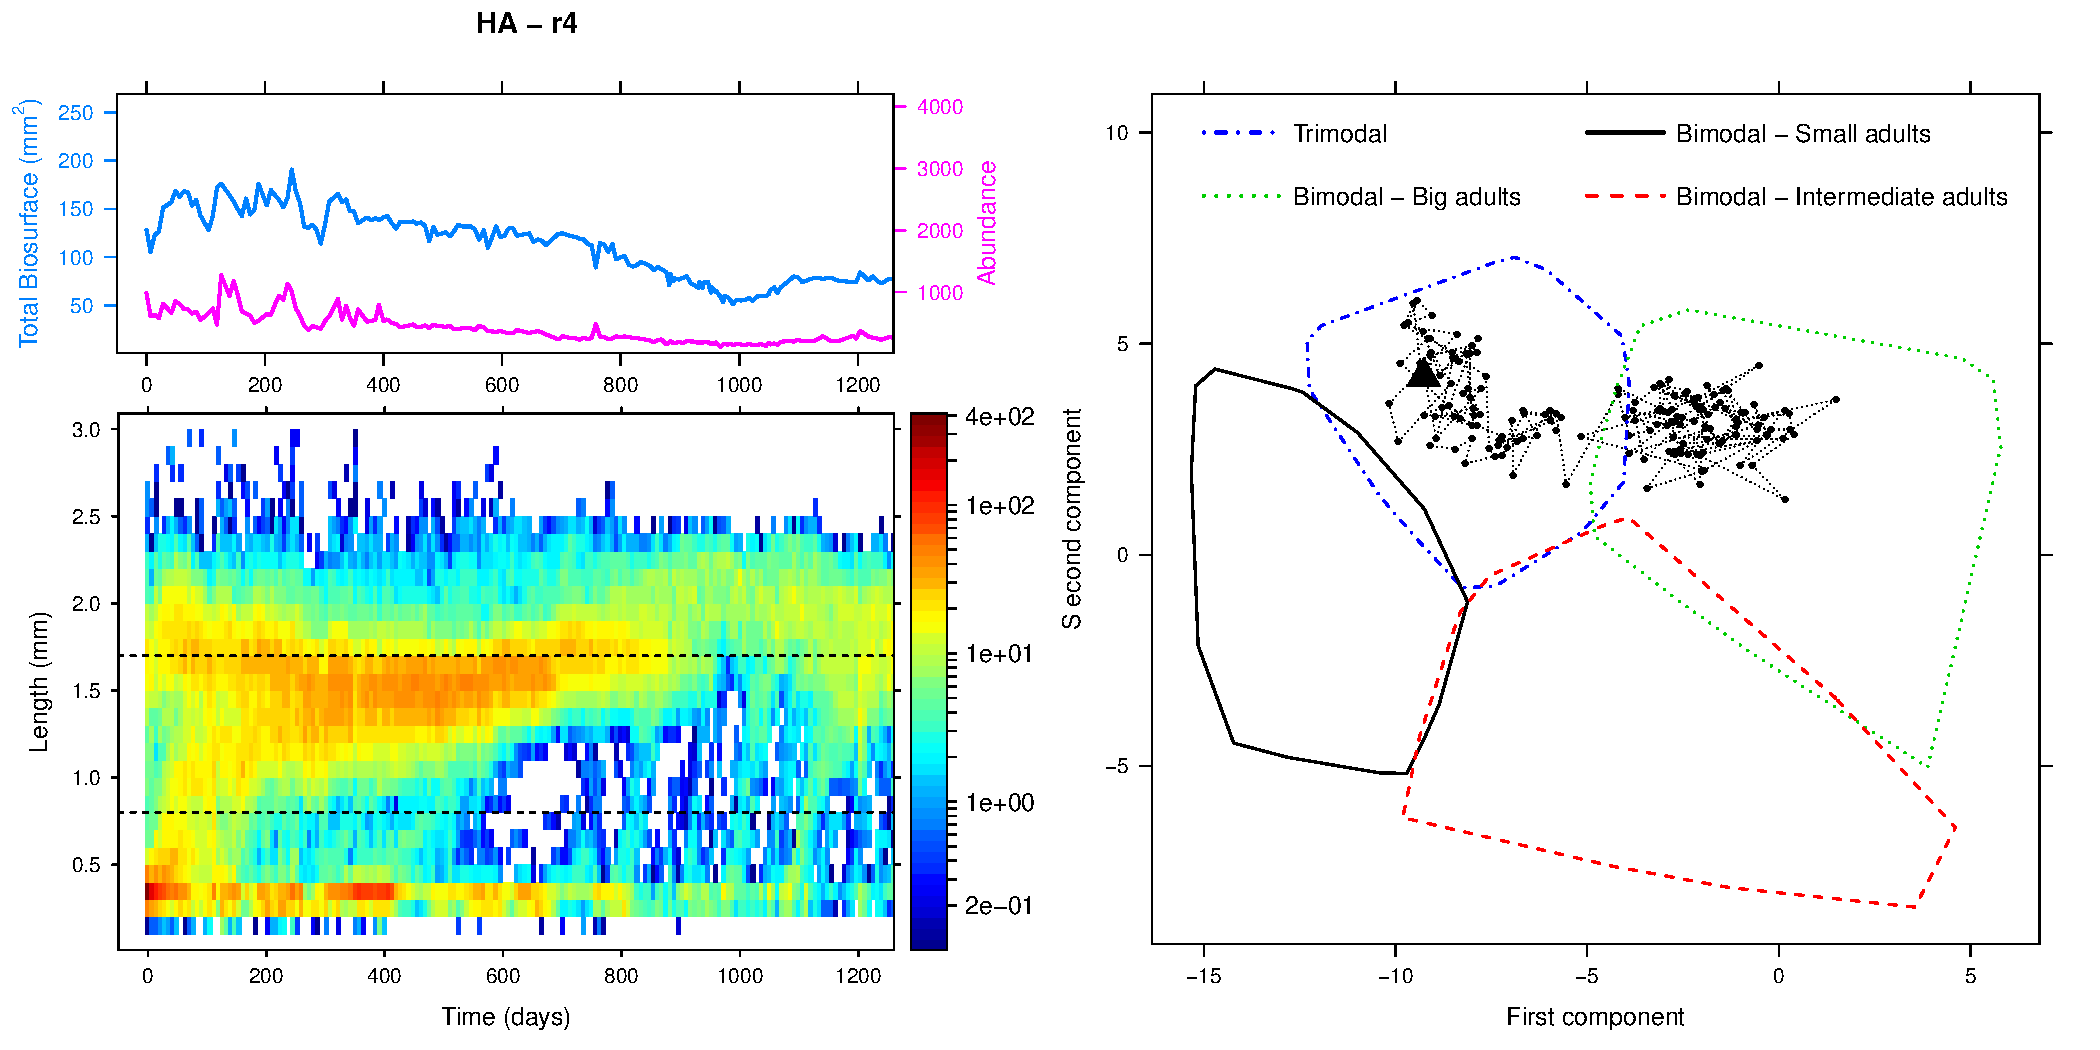
\includegraphics[height=0.33\textheight]{3-1_ChapExp1/Fig/HA-21-r4}

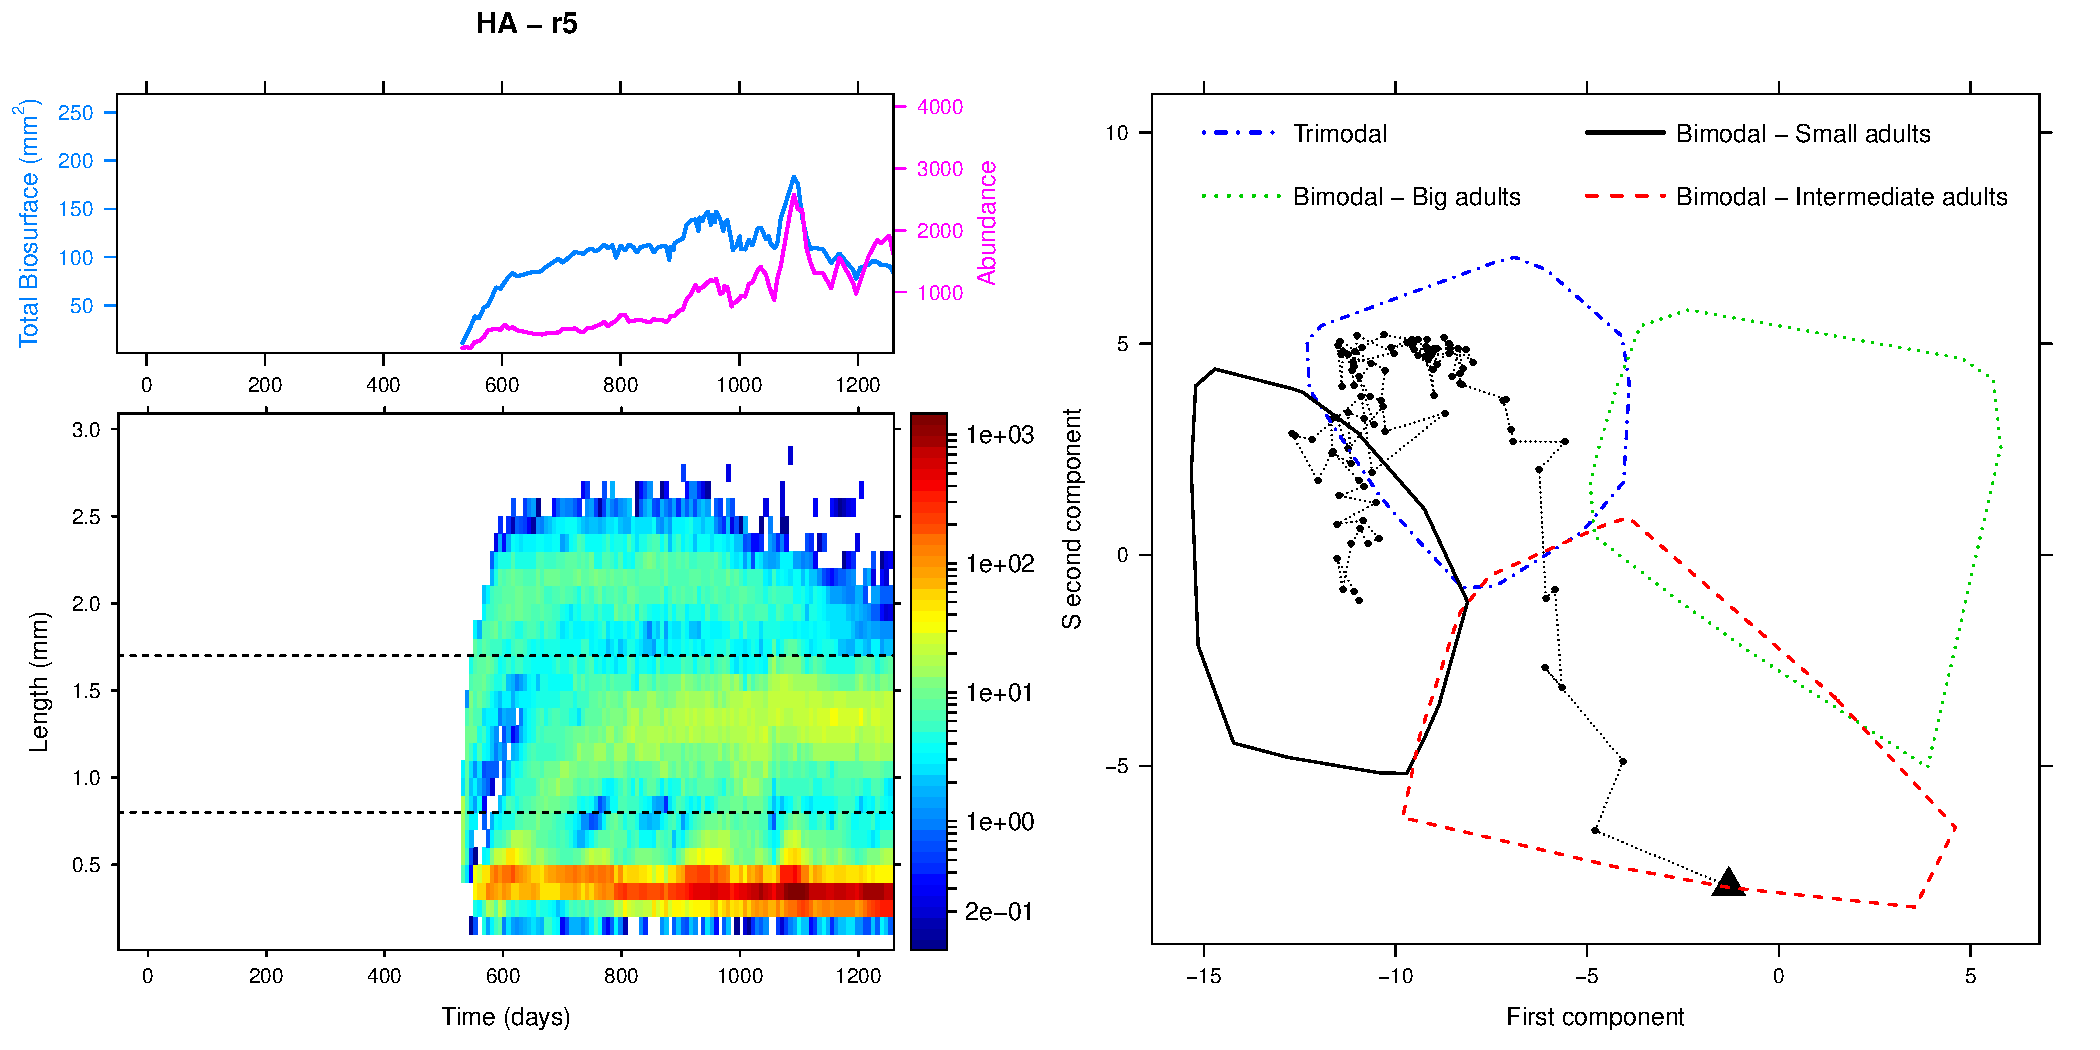
\includegraphics[height=0.33\textheight]{3-1_ChapExp1/Fig/HA-21-r5}

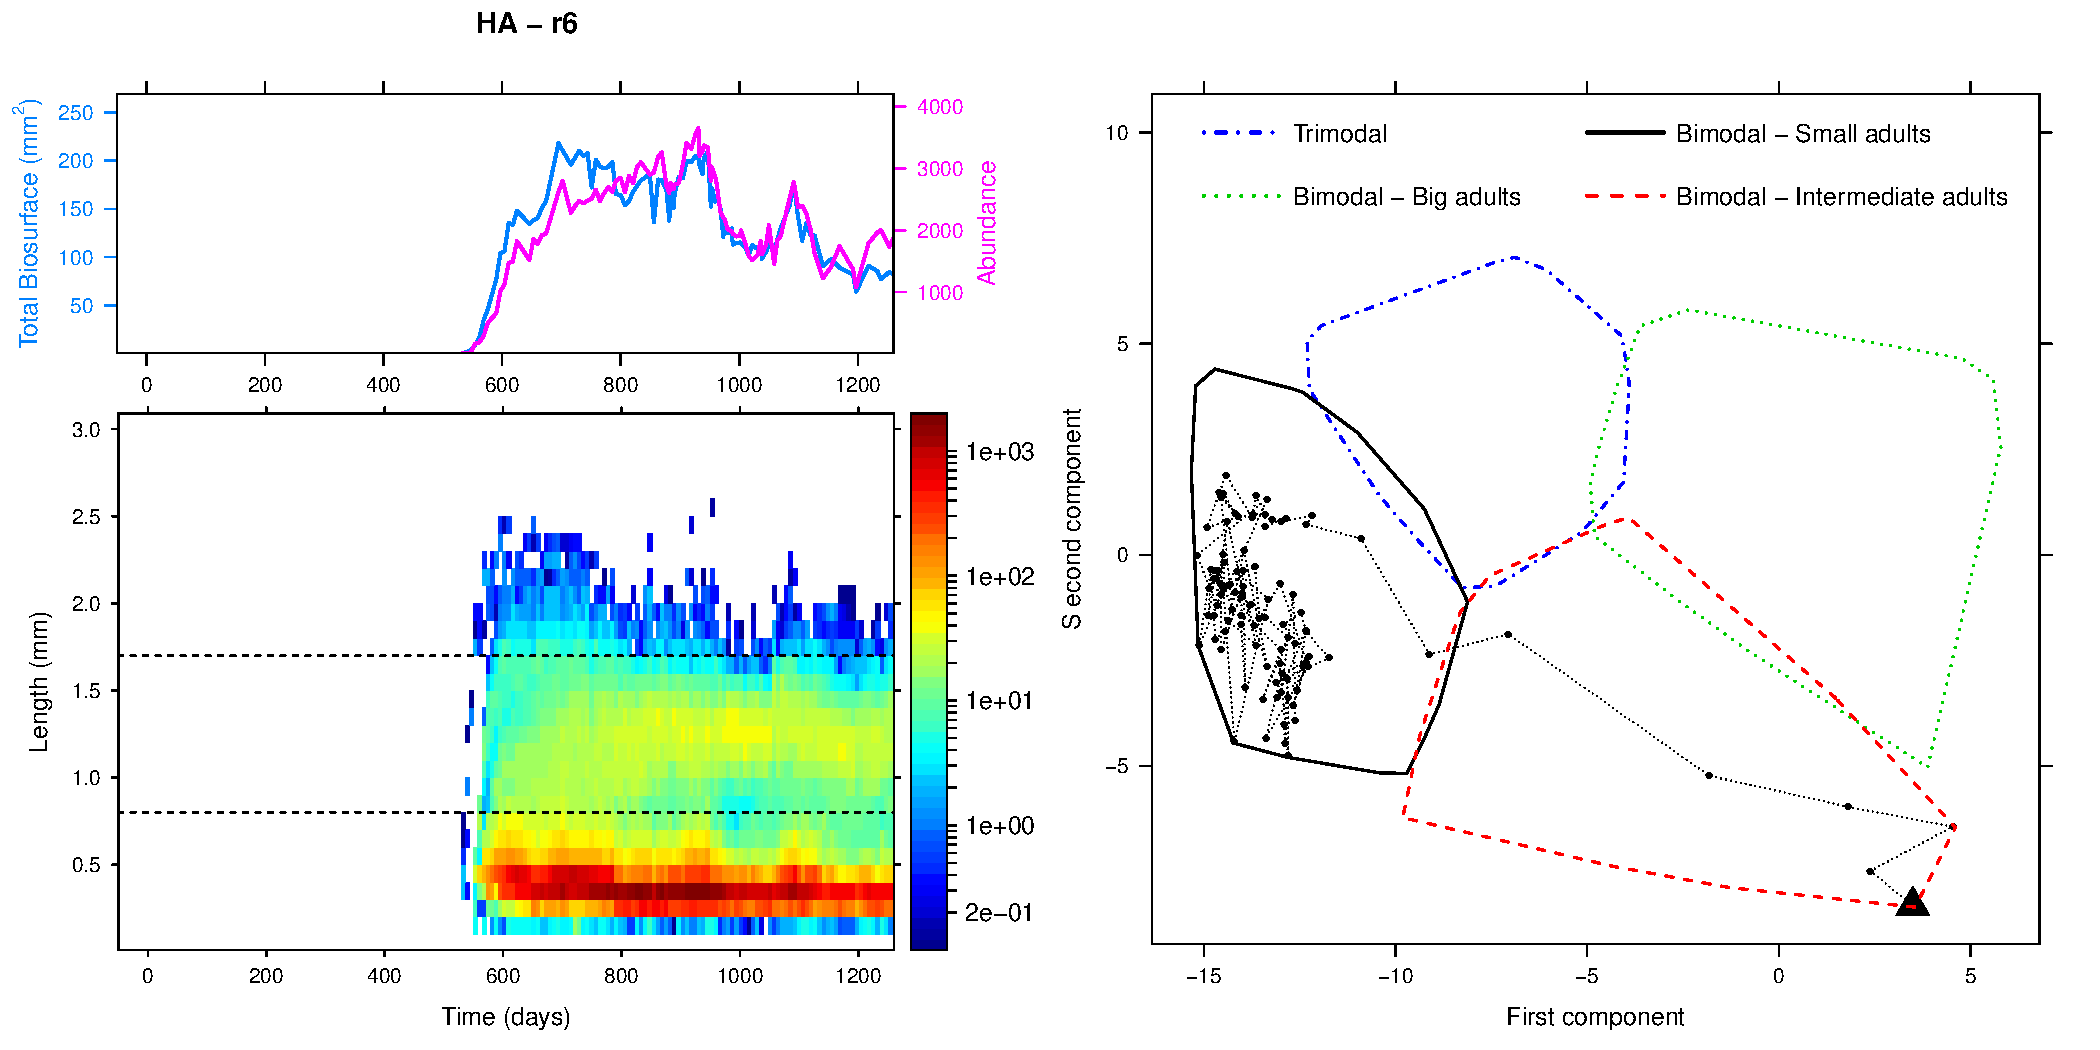
\includegraphics[height=0.33\textheight]{3-1_ChapExp1/Fig/HA-21-r6}

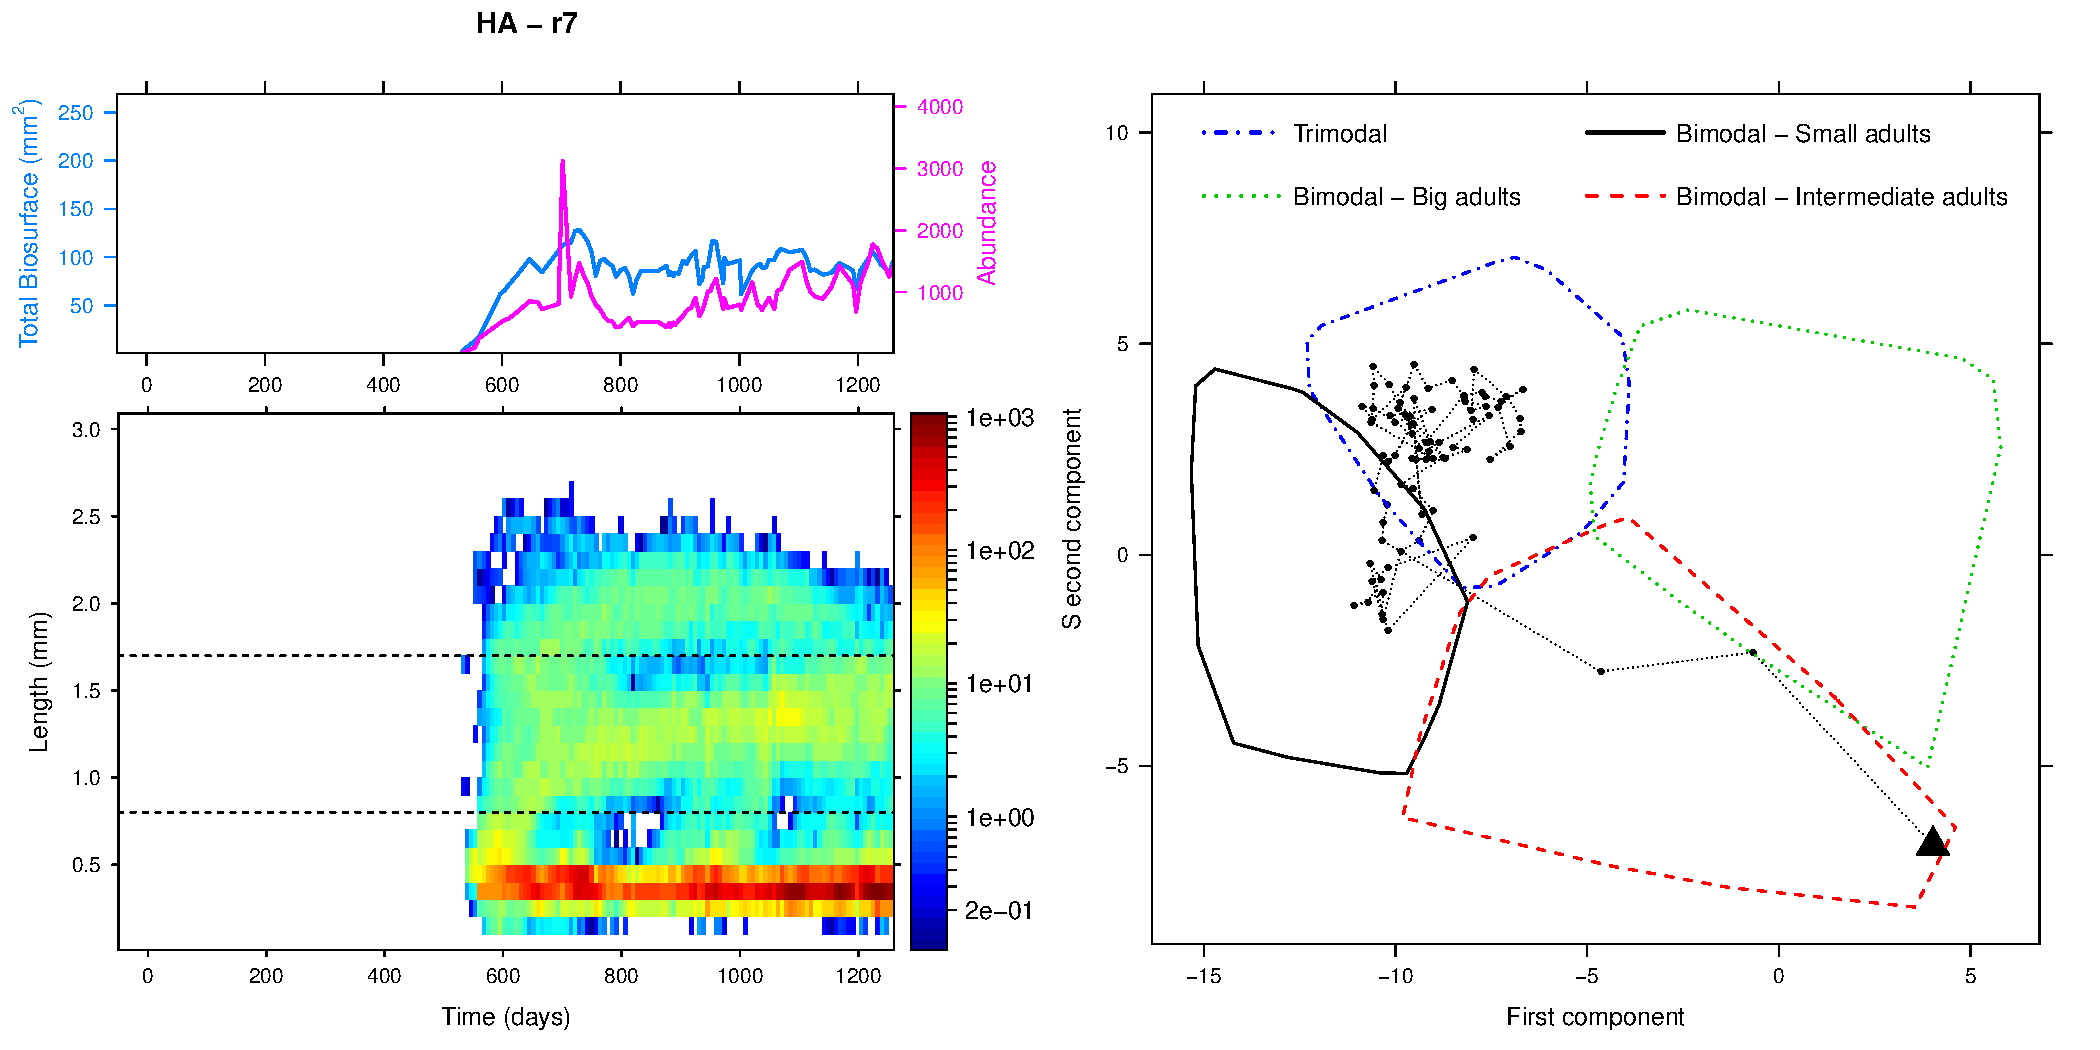
\includegraphics[height=0.33\textheight]{3-1_ChapExp1/Fig/HA-21-r7}

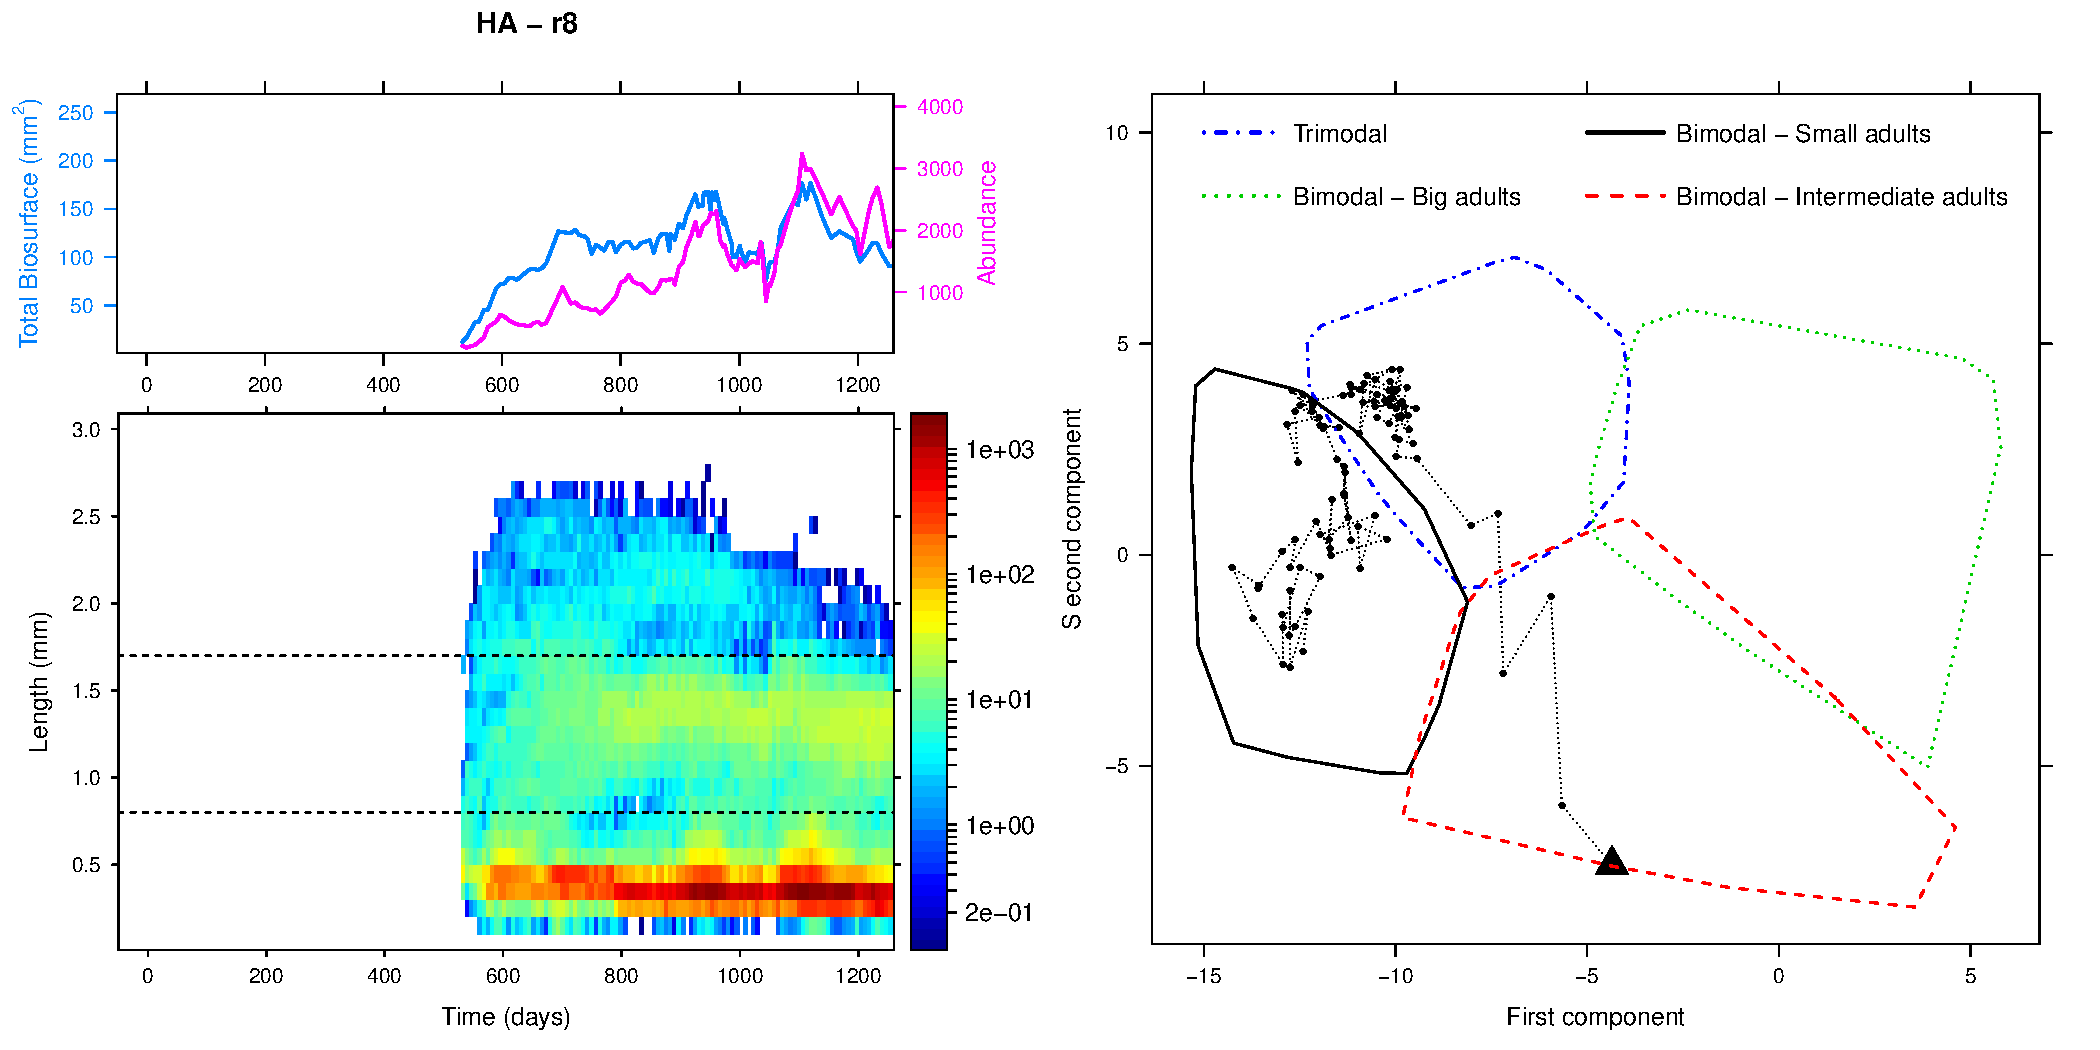
\includegraphics[height=0.33\textheight]{3-1_ChapExp1/Fig/HA-21-r8}

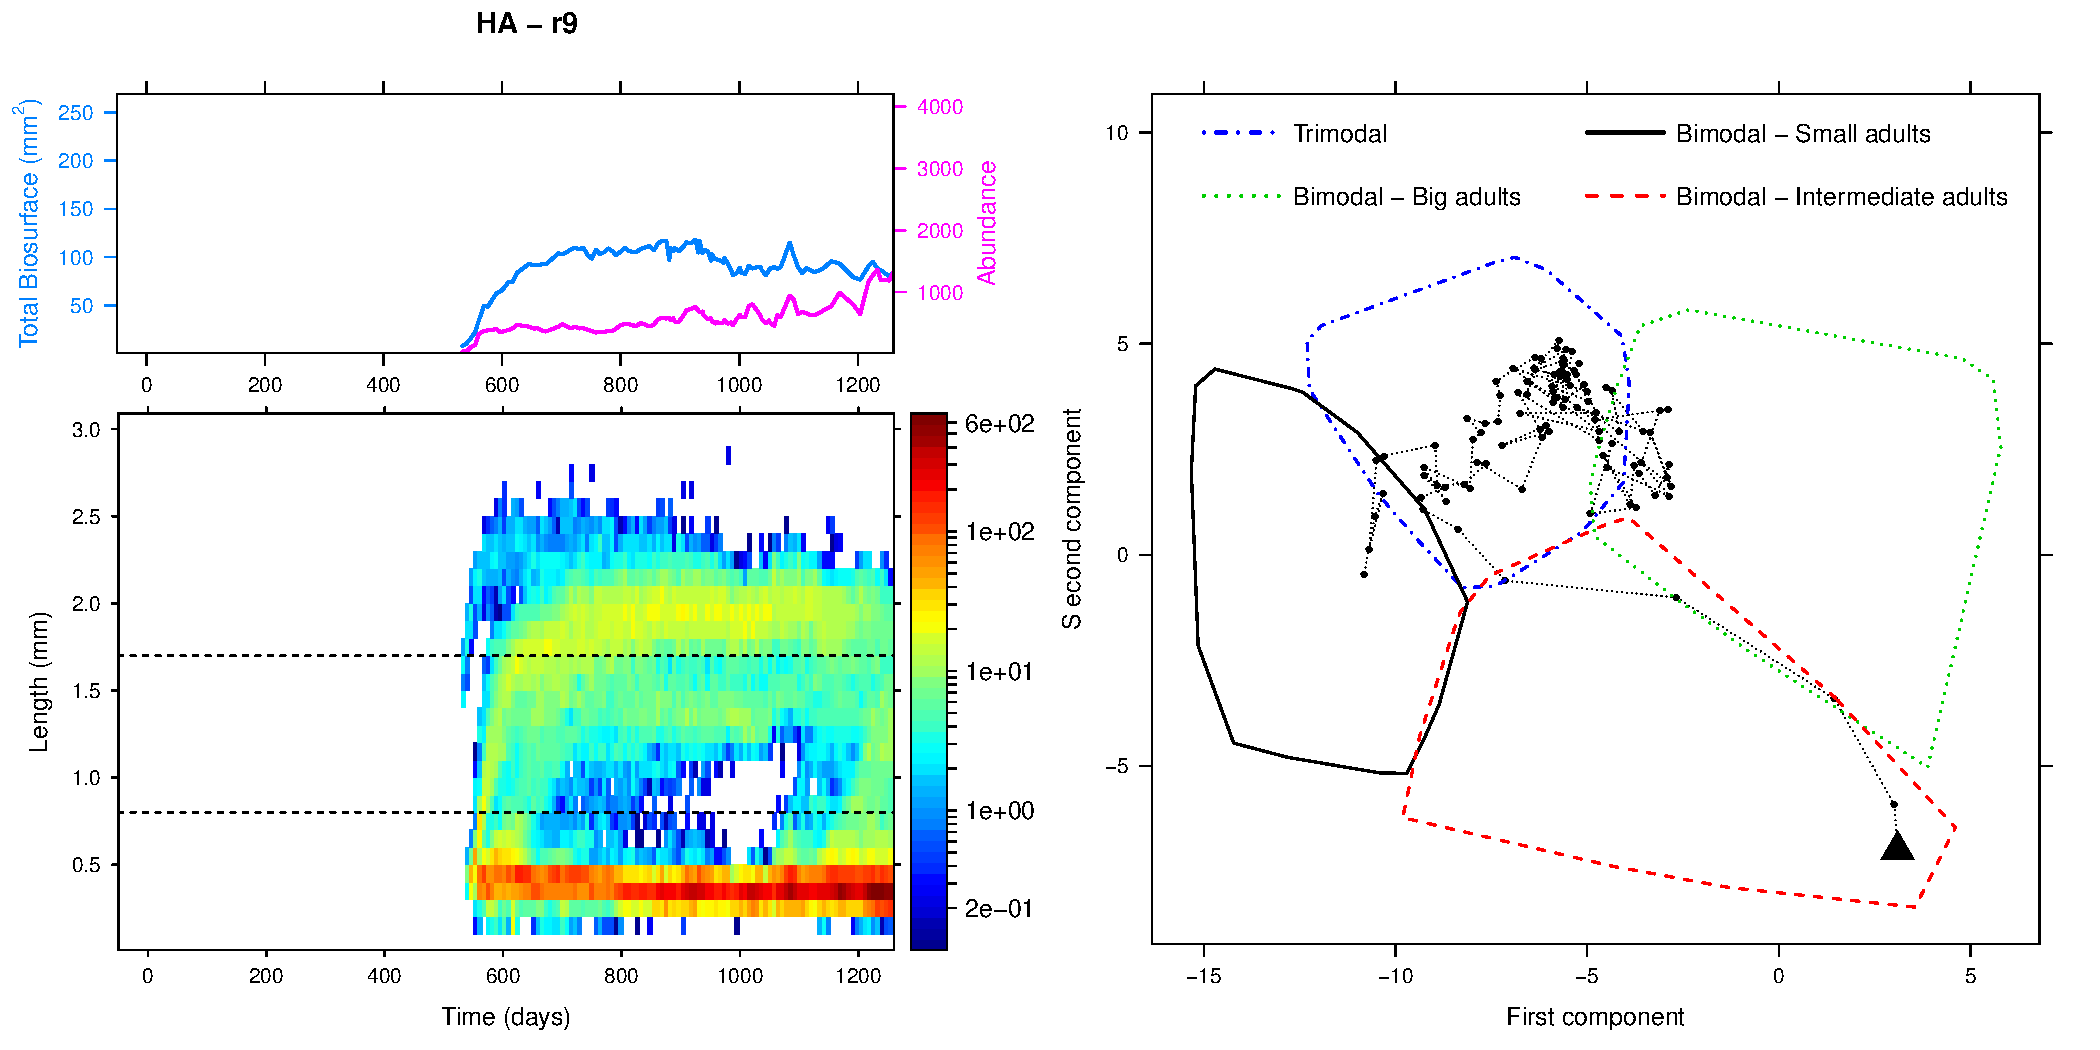
\includegraphics[height=0.33\textheight]{3-1_ChapExp1/Fig/HA-21-r9}

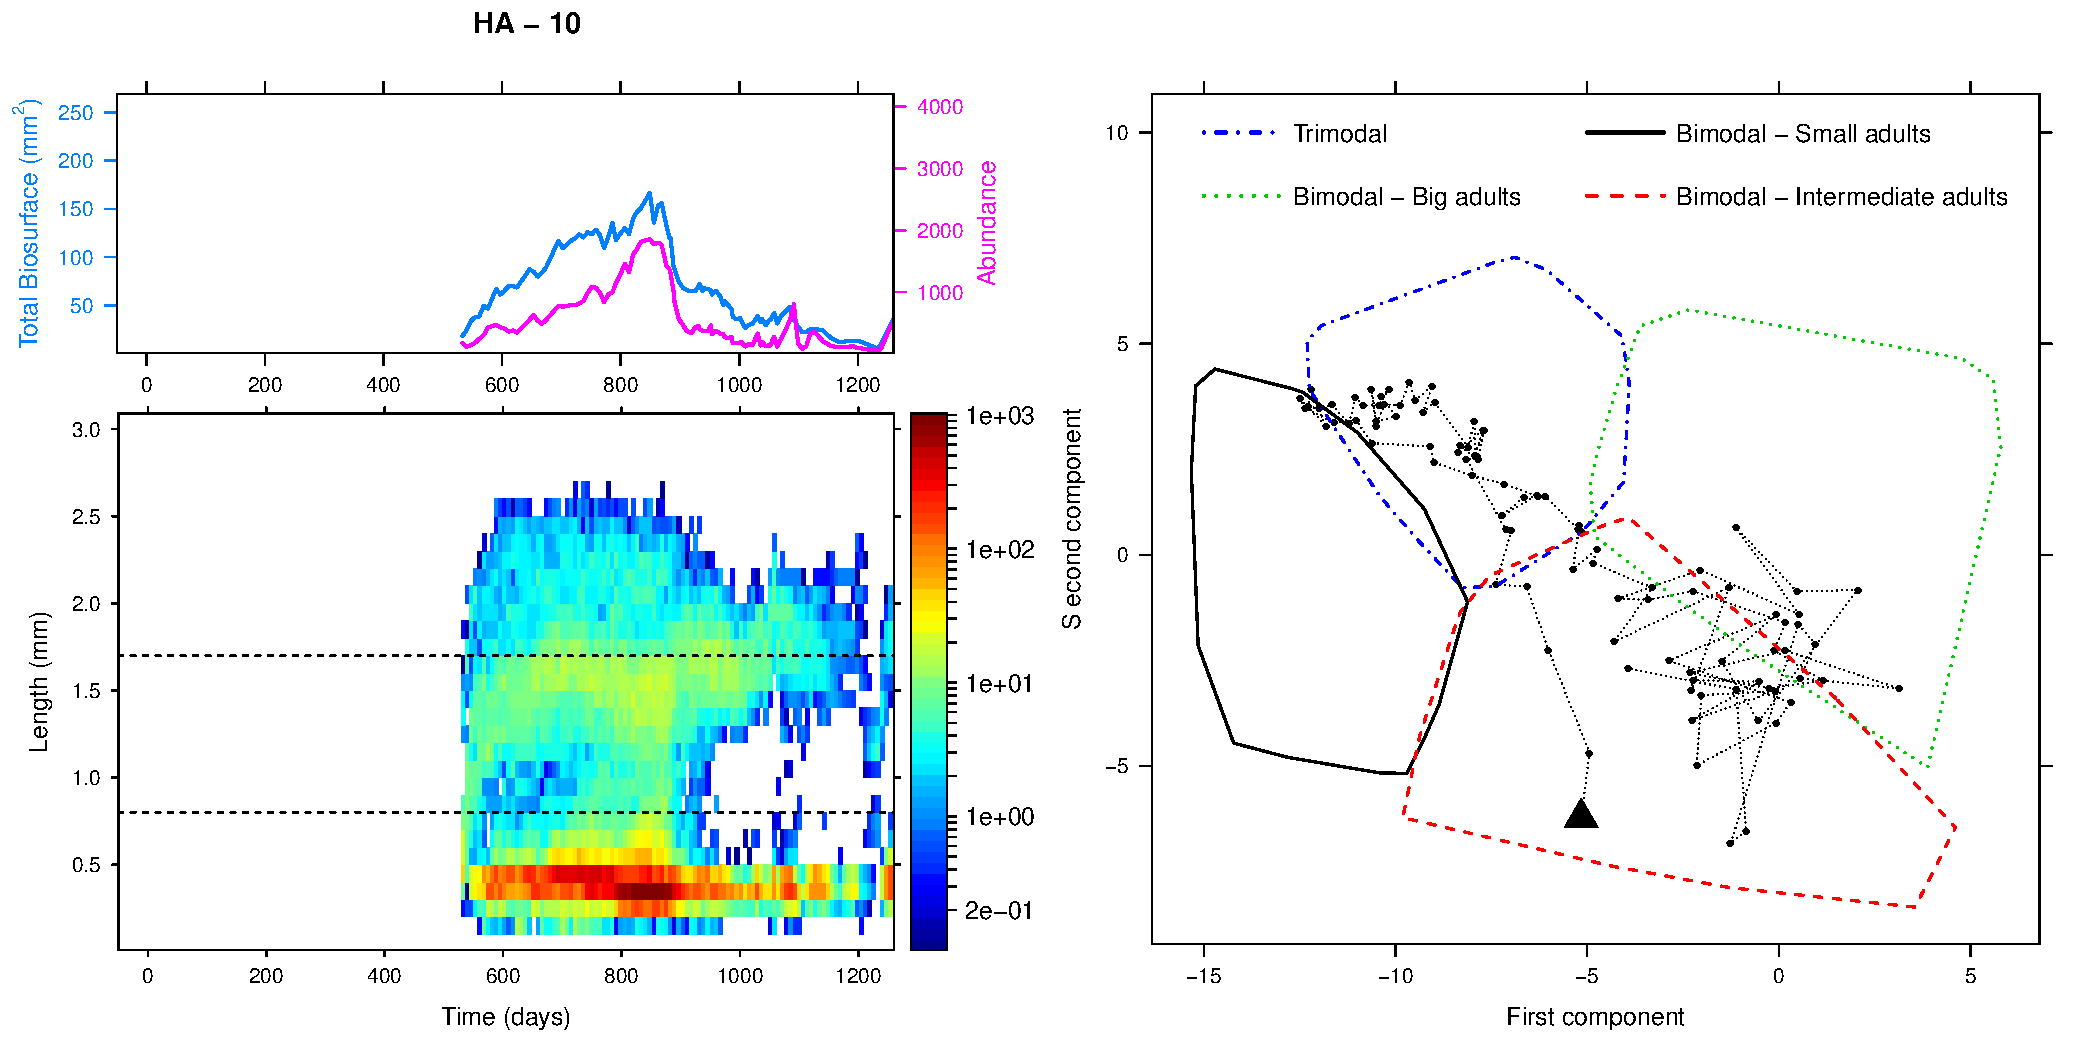
\includegraphics[height=0.33\textheight]{3-1_ChapExp1/Fig/HA-21-10}

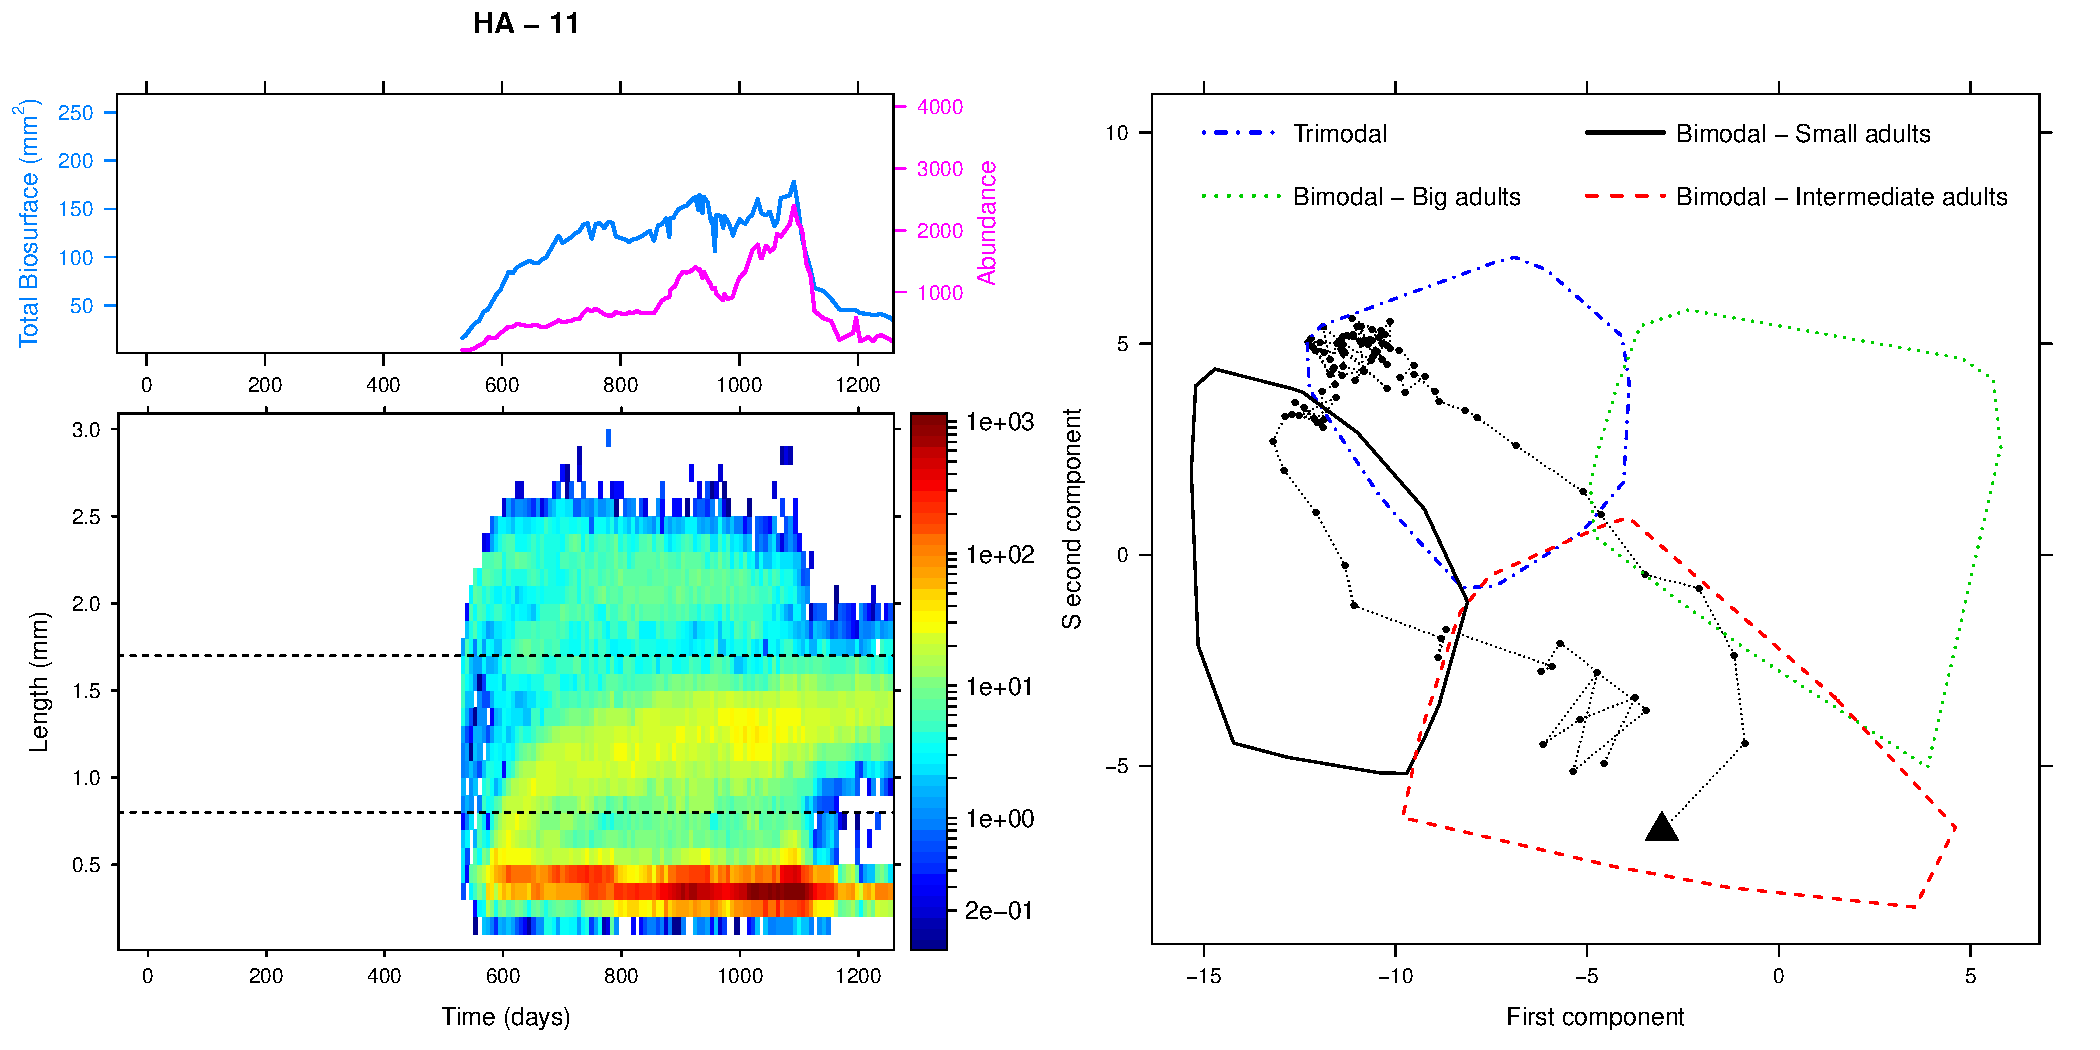
\includegraphics[height=0.33\textheight]{3-1_ChapExp1/Fig/HA-21-11}

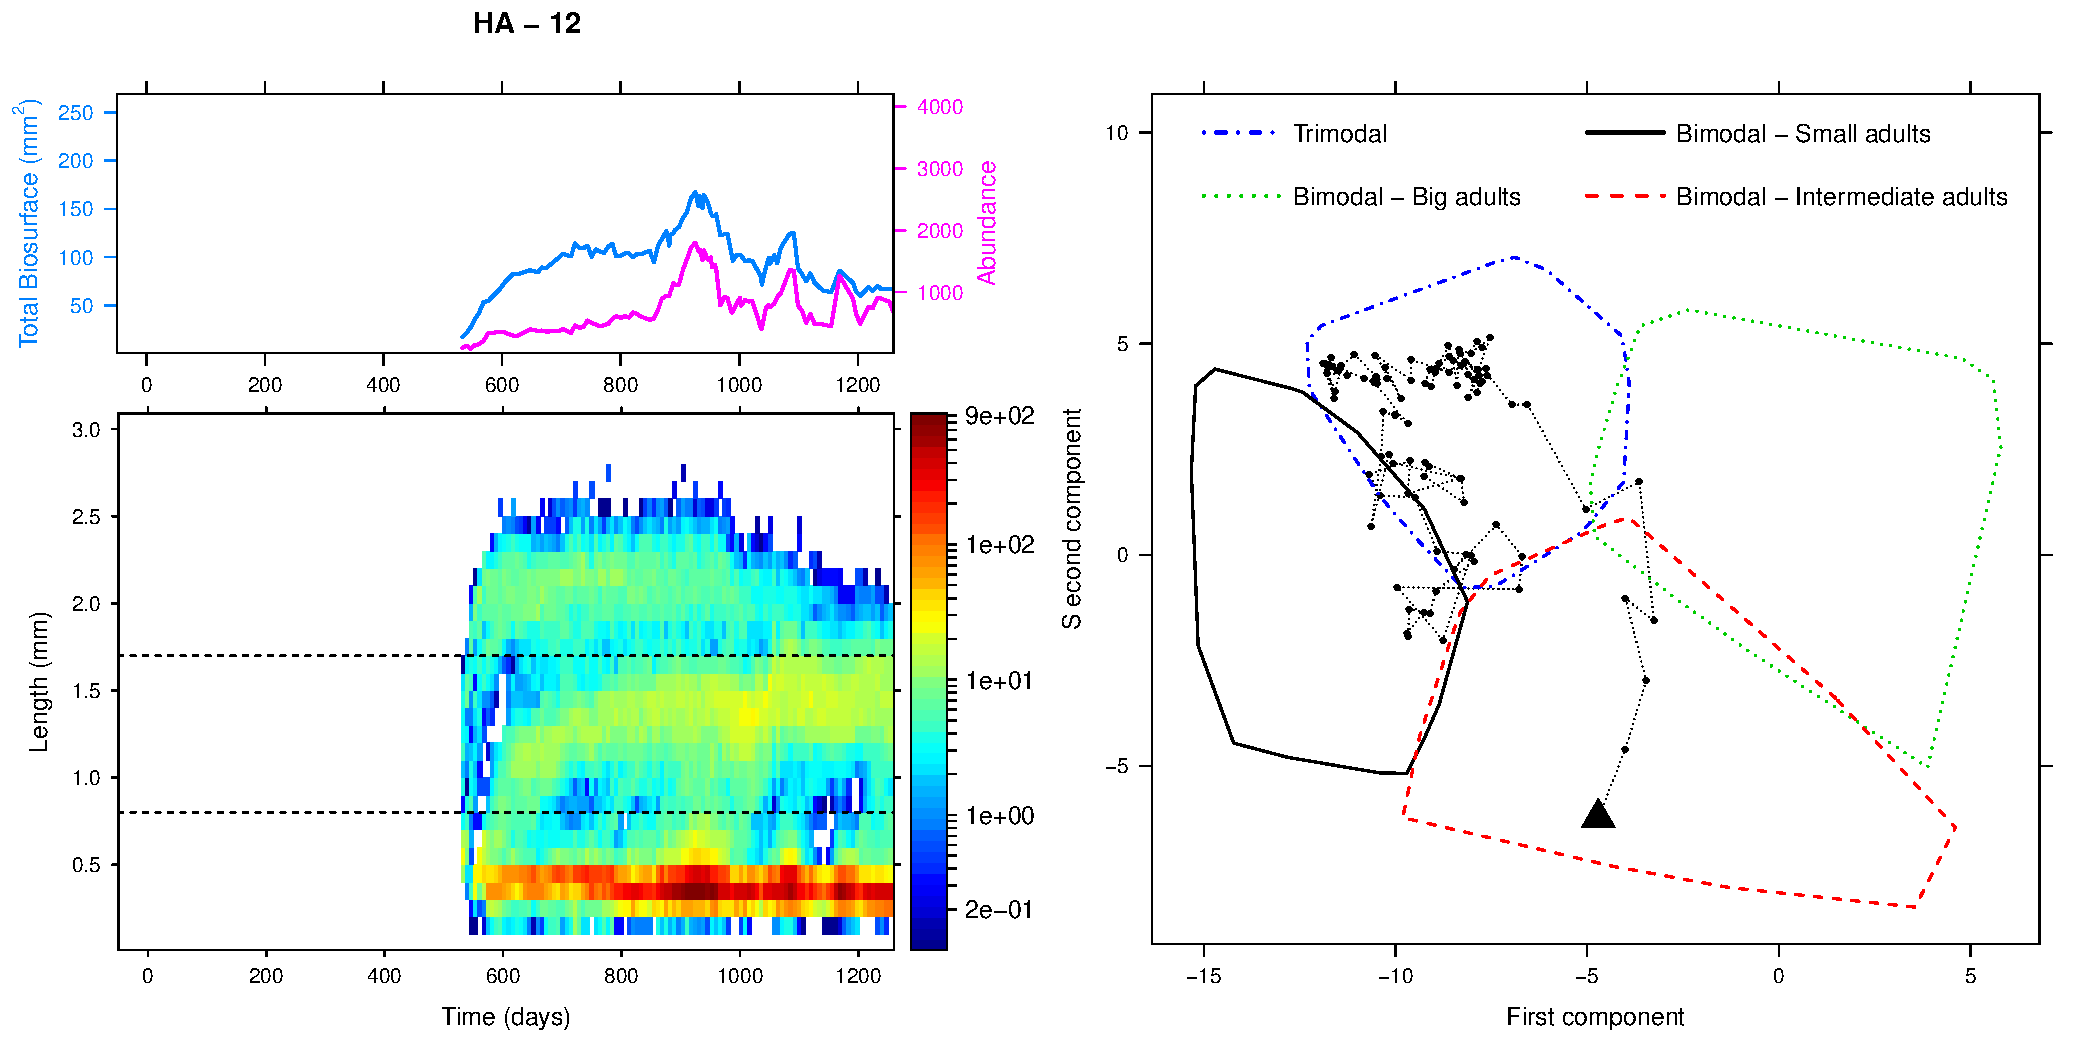
\includegraphics[height=0.33\textheight]{3-1_ChapExp1/Fig/HA-21-12}

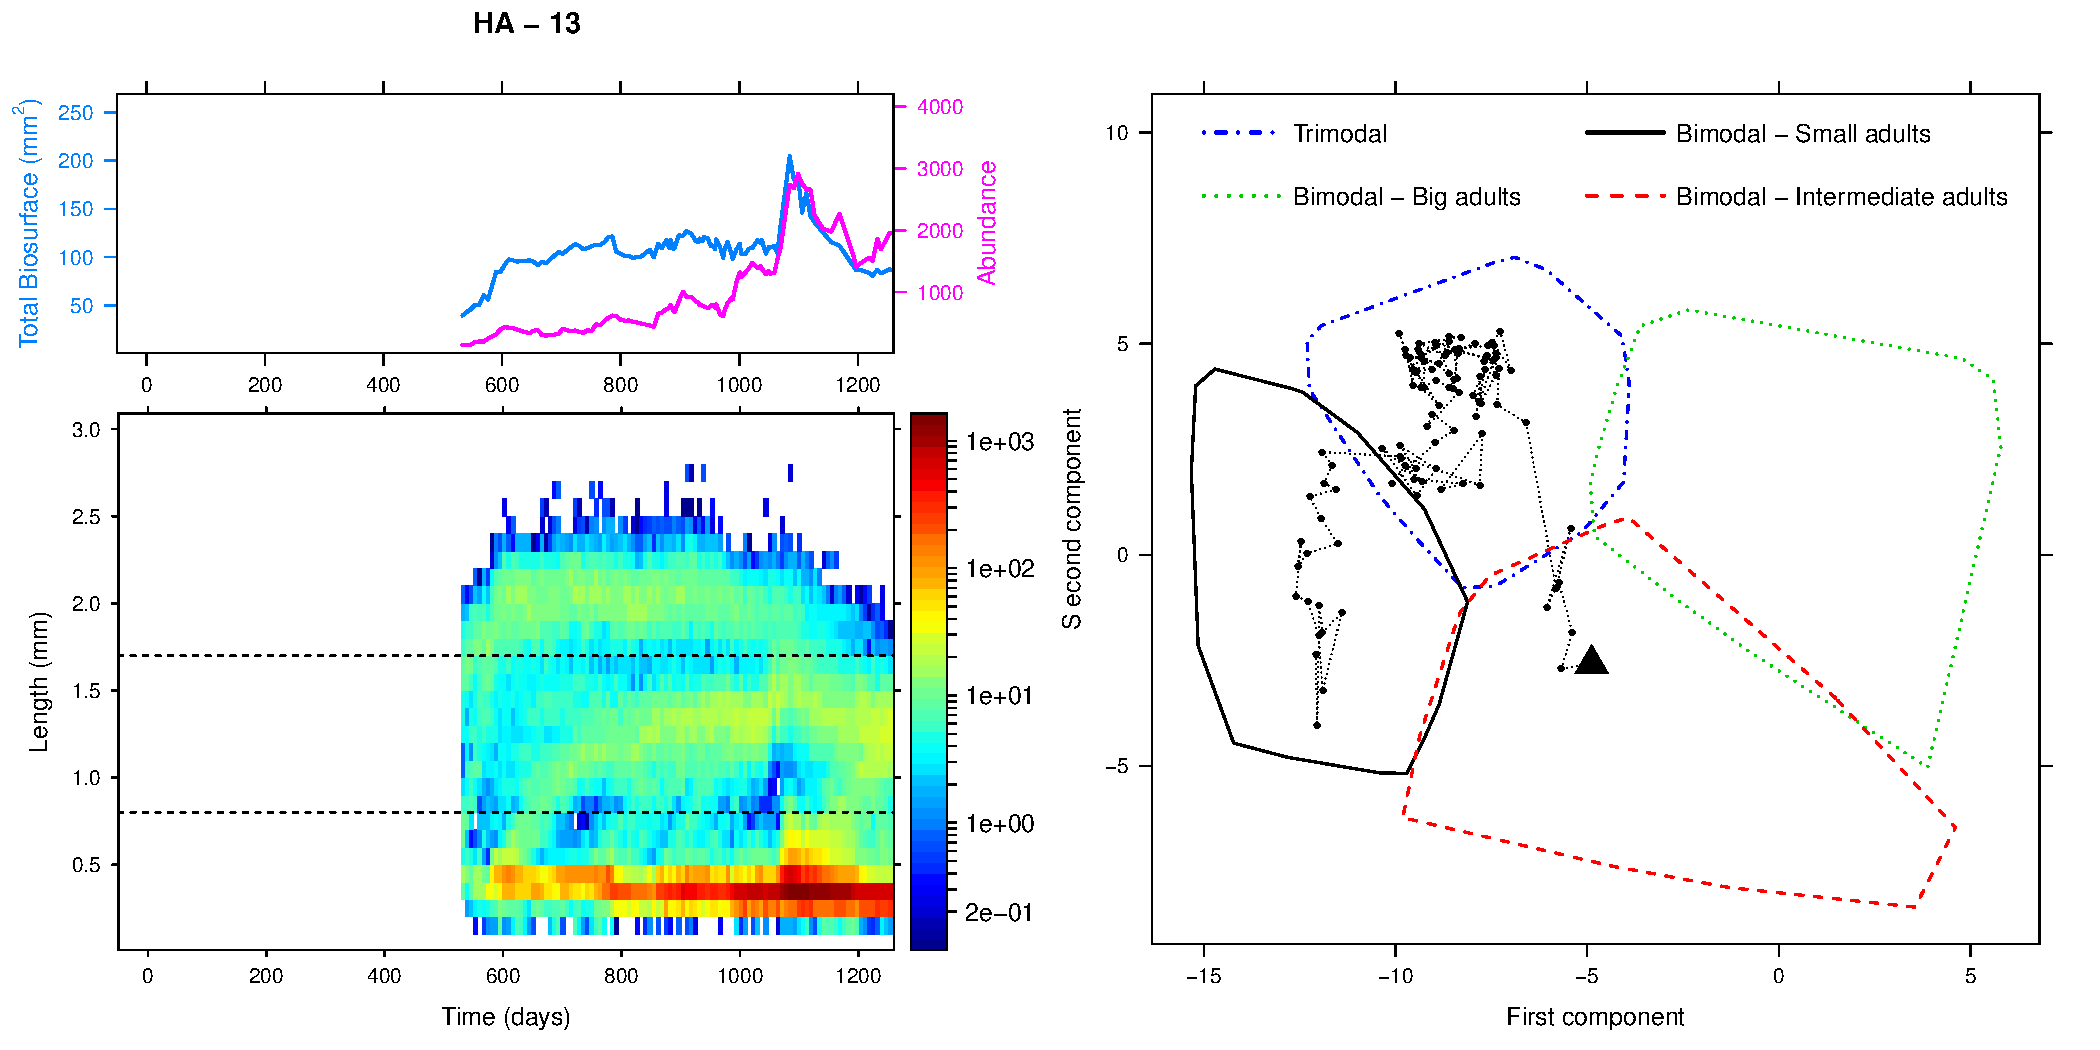
\includegraphics[height=0.33\textheight]{3-1_ChapExp1/Fig/HA-21-13}

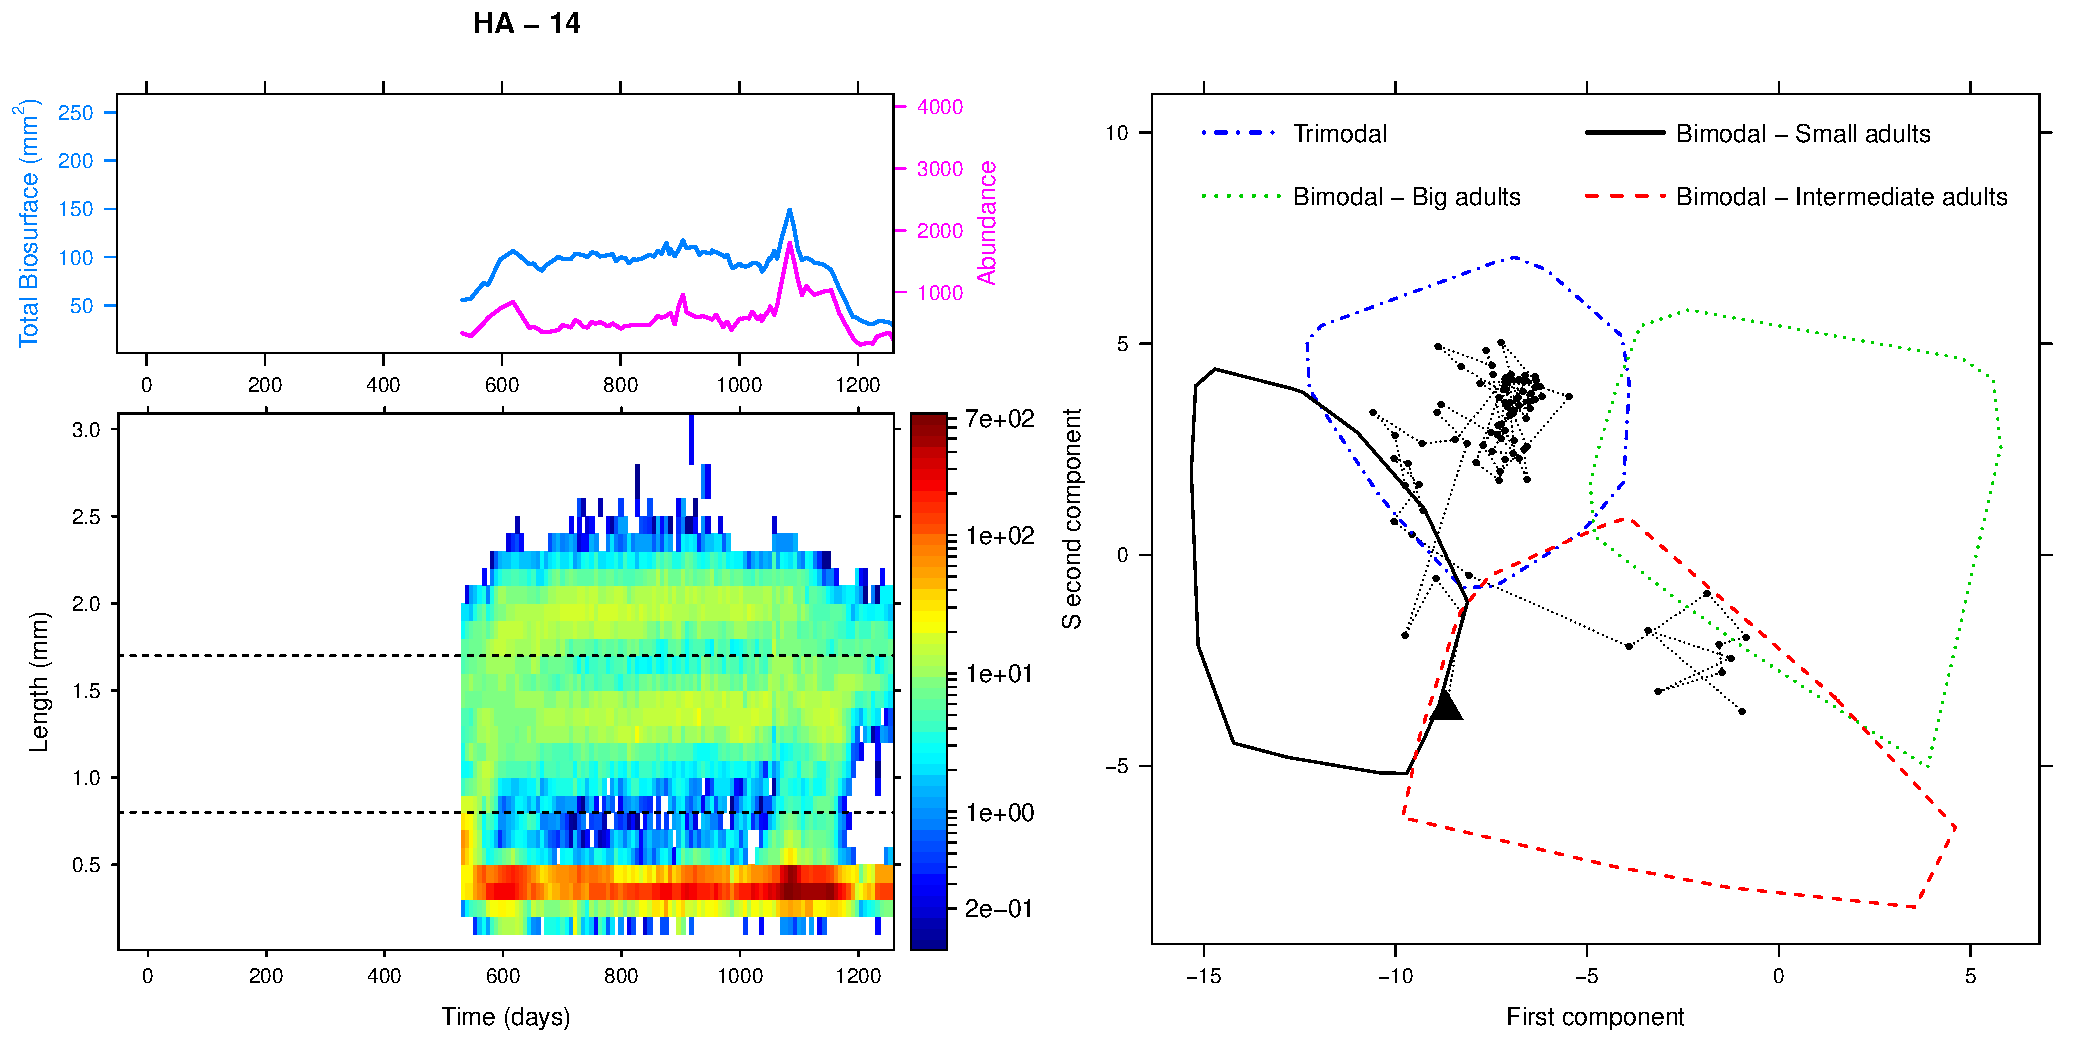
\includegraphics[height=0.33\textheight]{3-1_ChapExp1/Fig/HA-21-14}

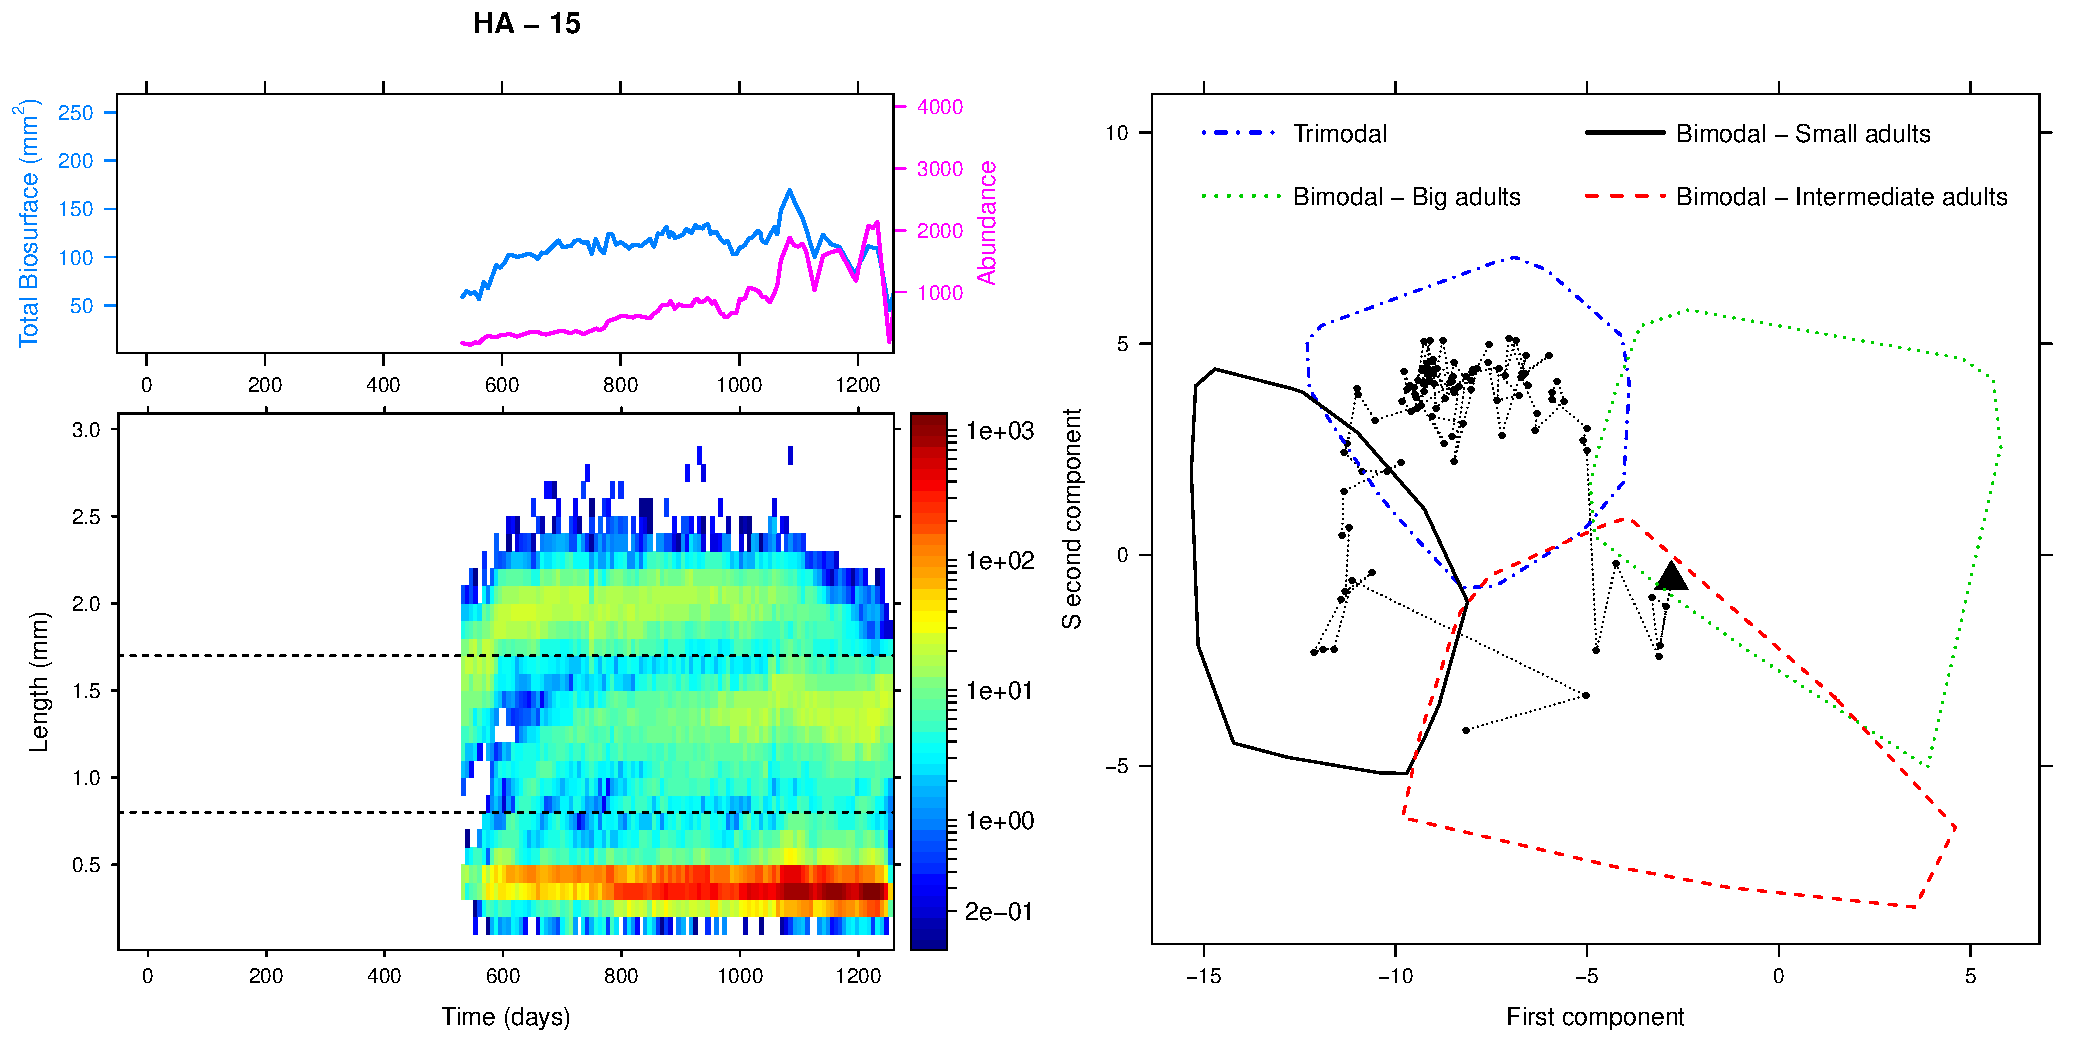
\includegraphics[height=0.33\textheight]{3-1_ChapExp1/Fig/HA-21-15}

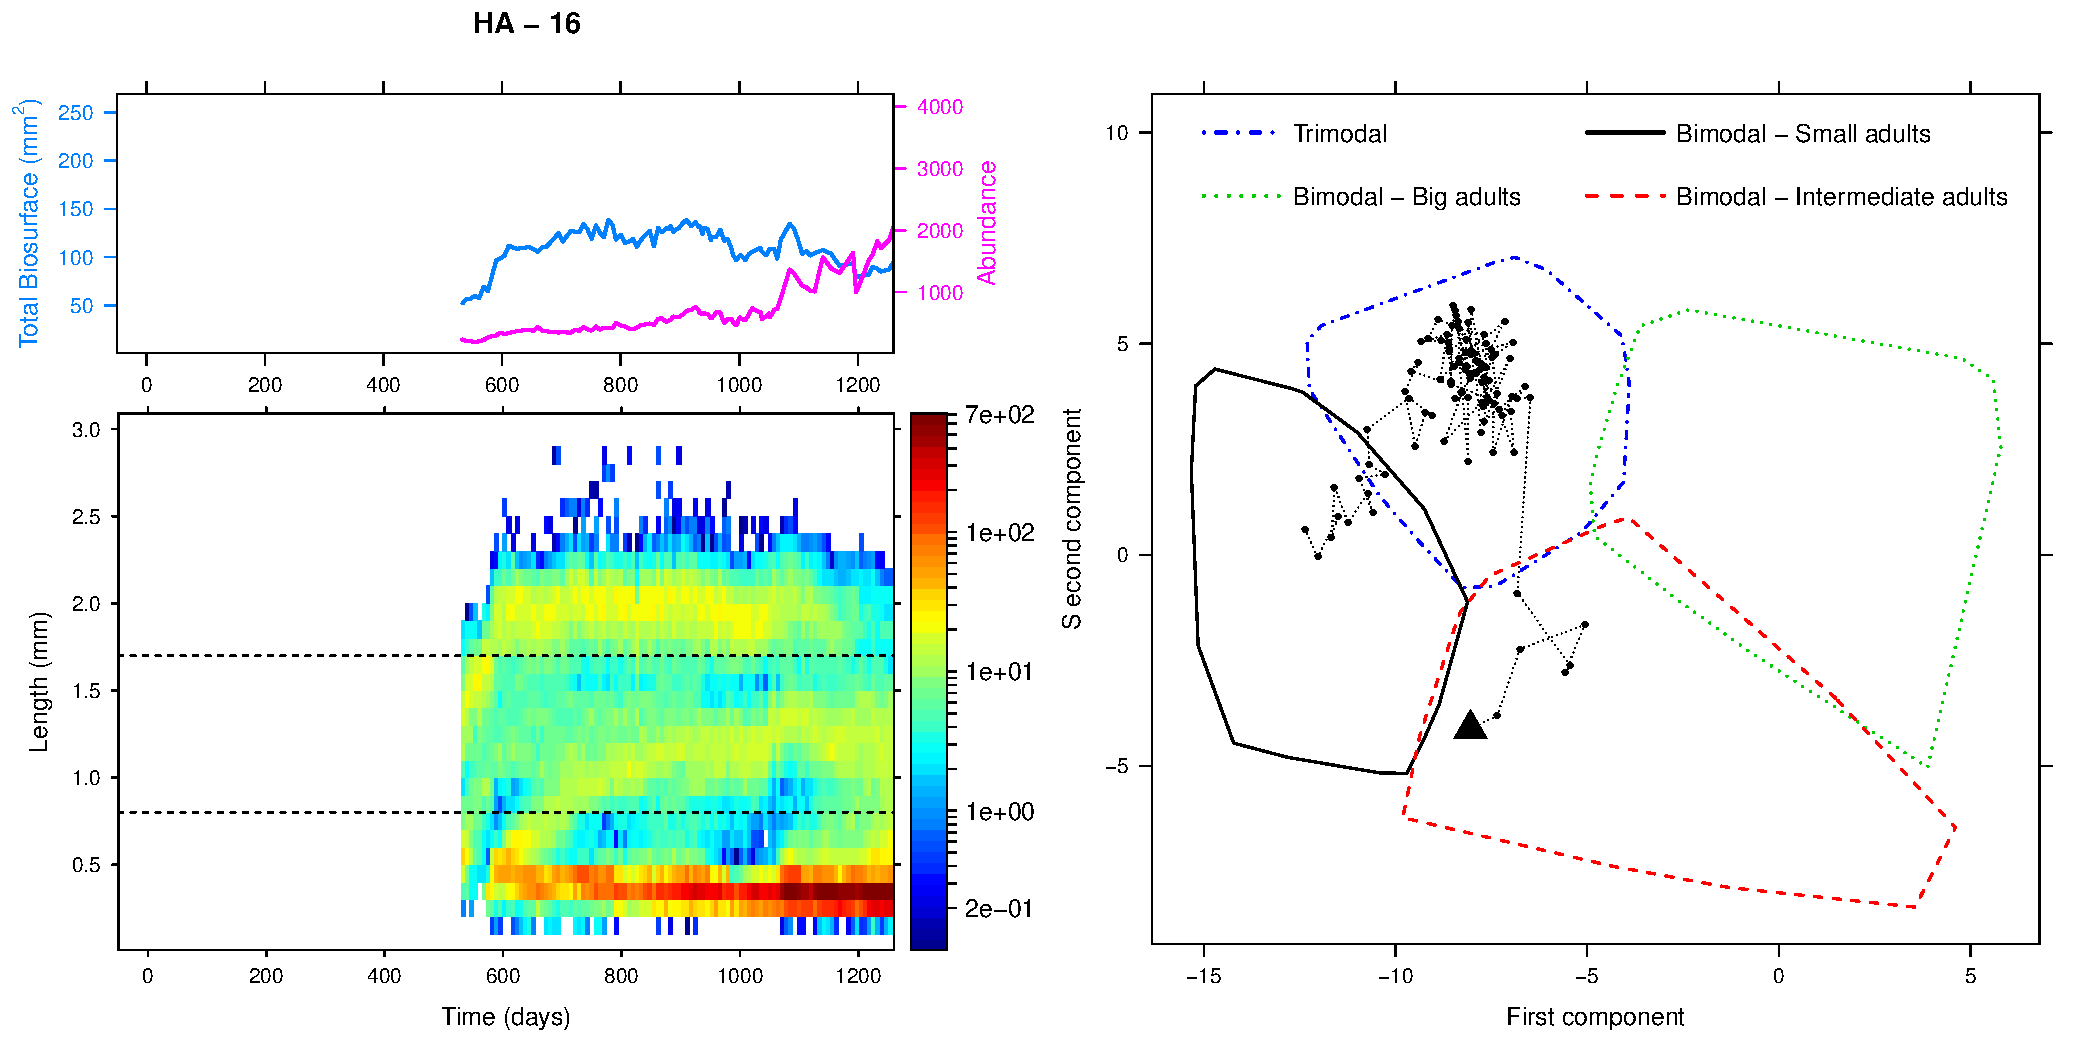
\includegraphics[height=0.33\textheight]{3-1_ChapExp1/Fig/HA-21-16}

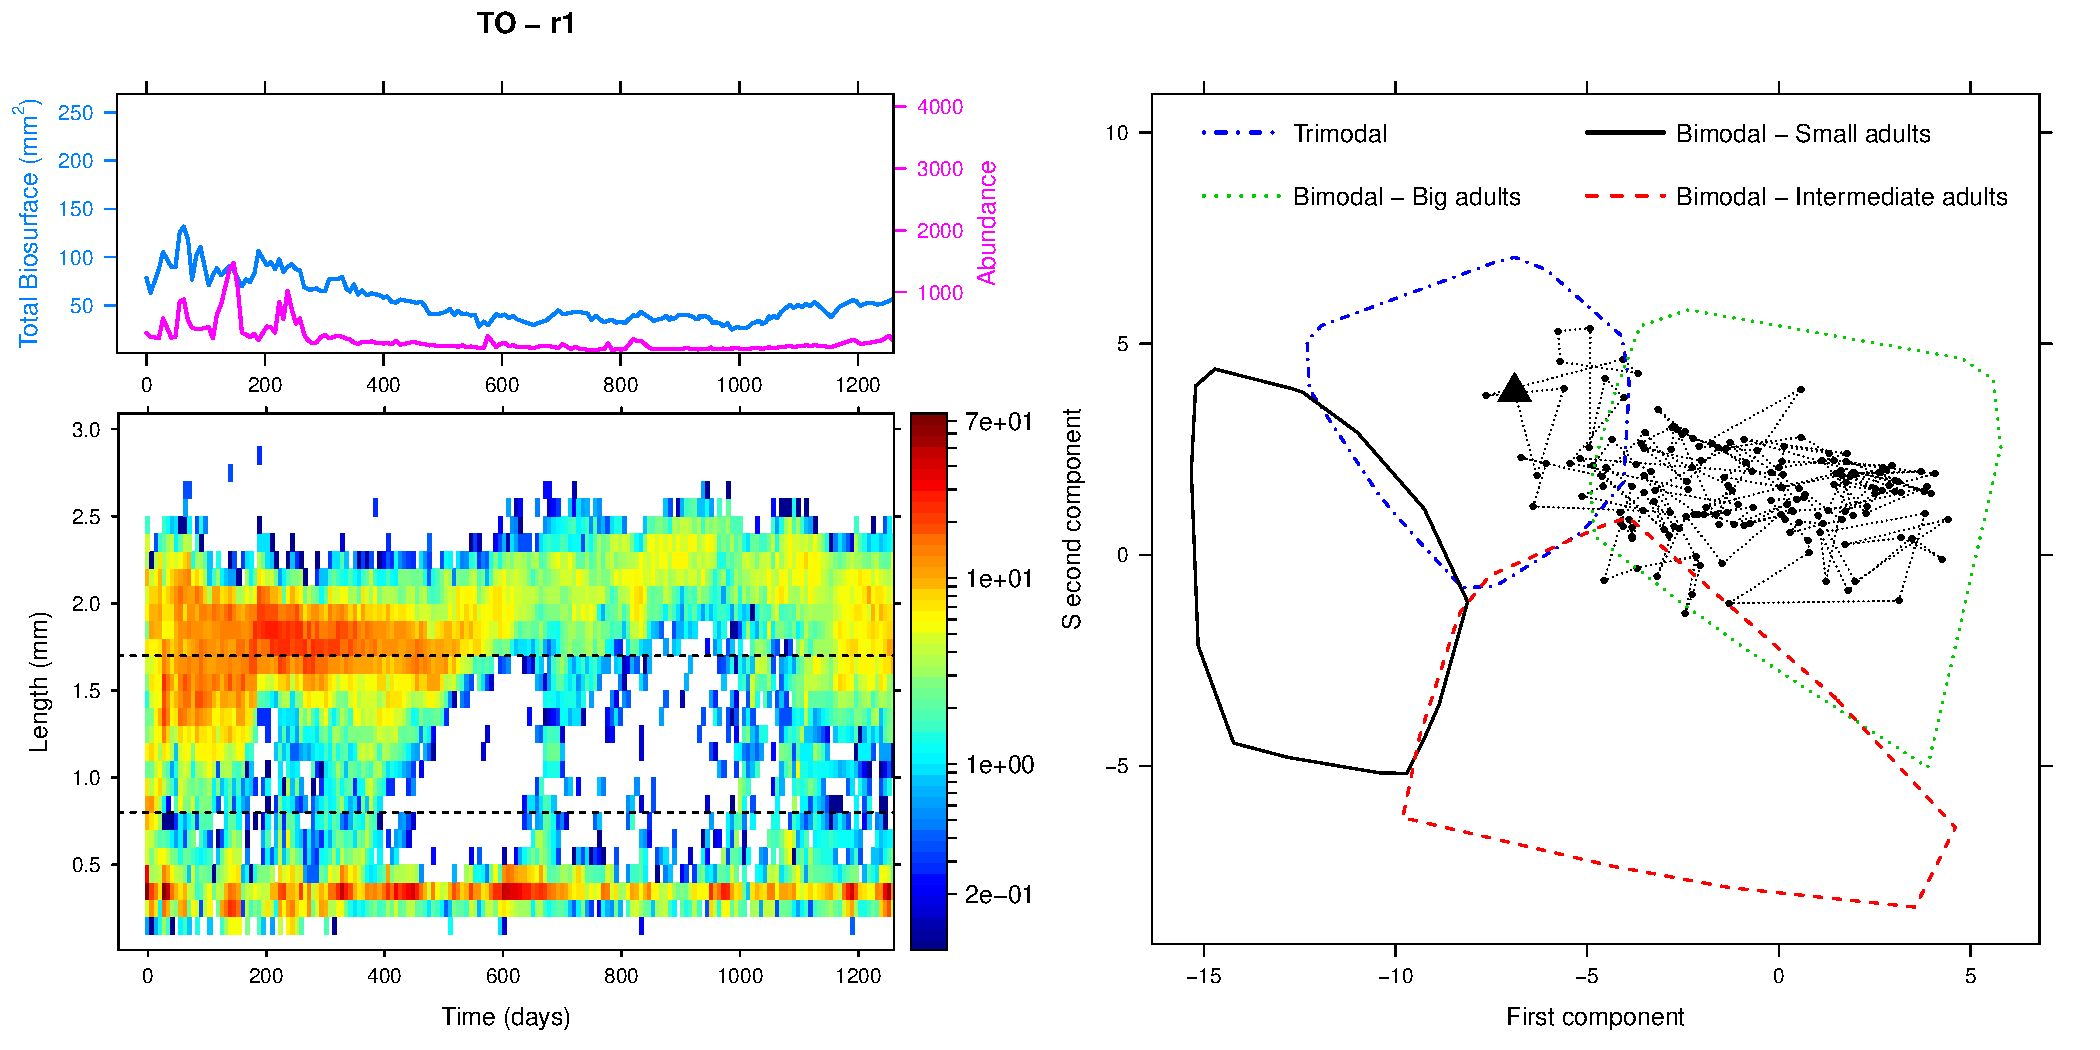
\includegraphics[height=0.33\textheight]{3-1_ChapExp1/Fig/TO-21-r1}

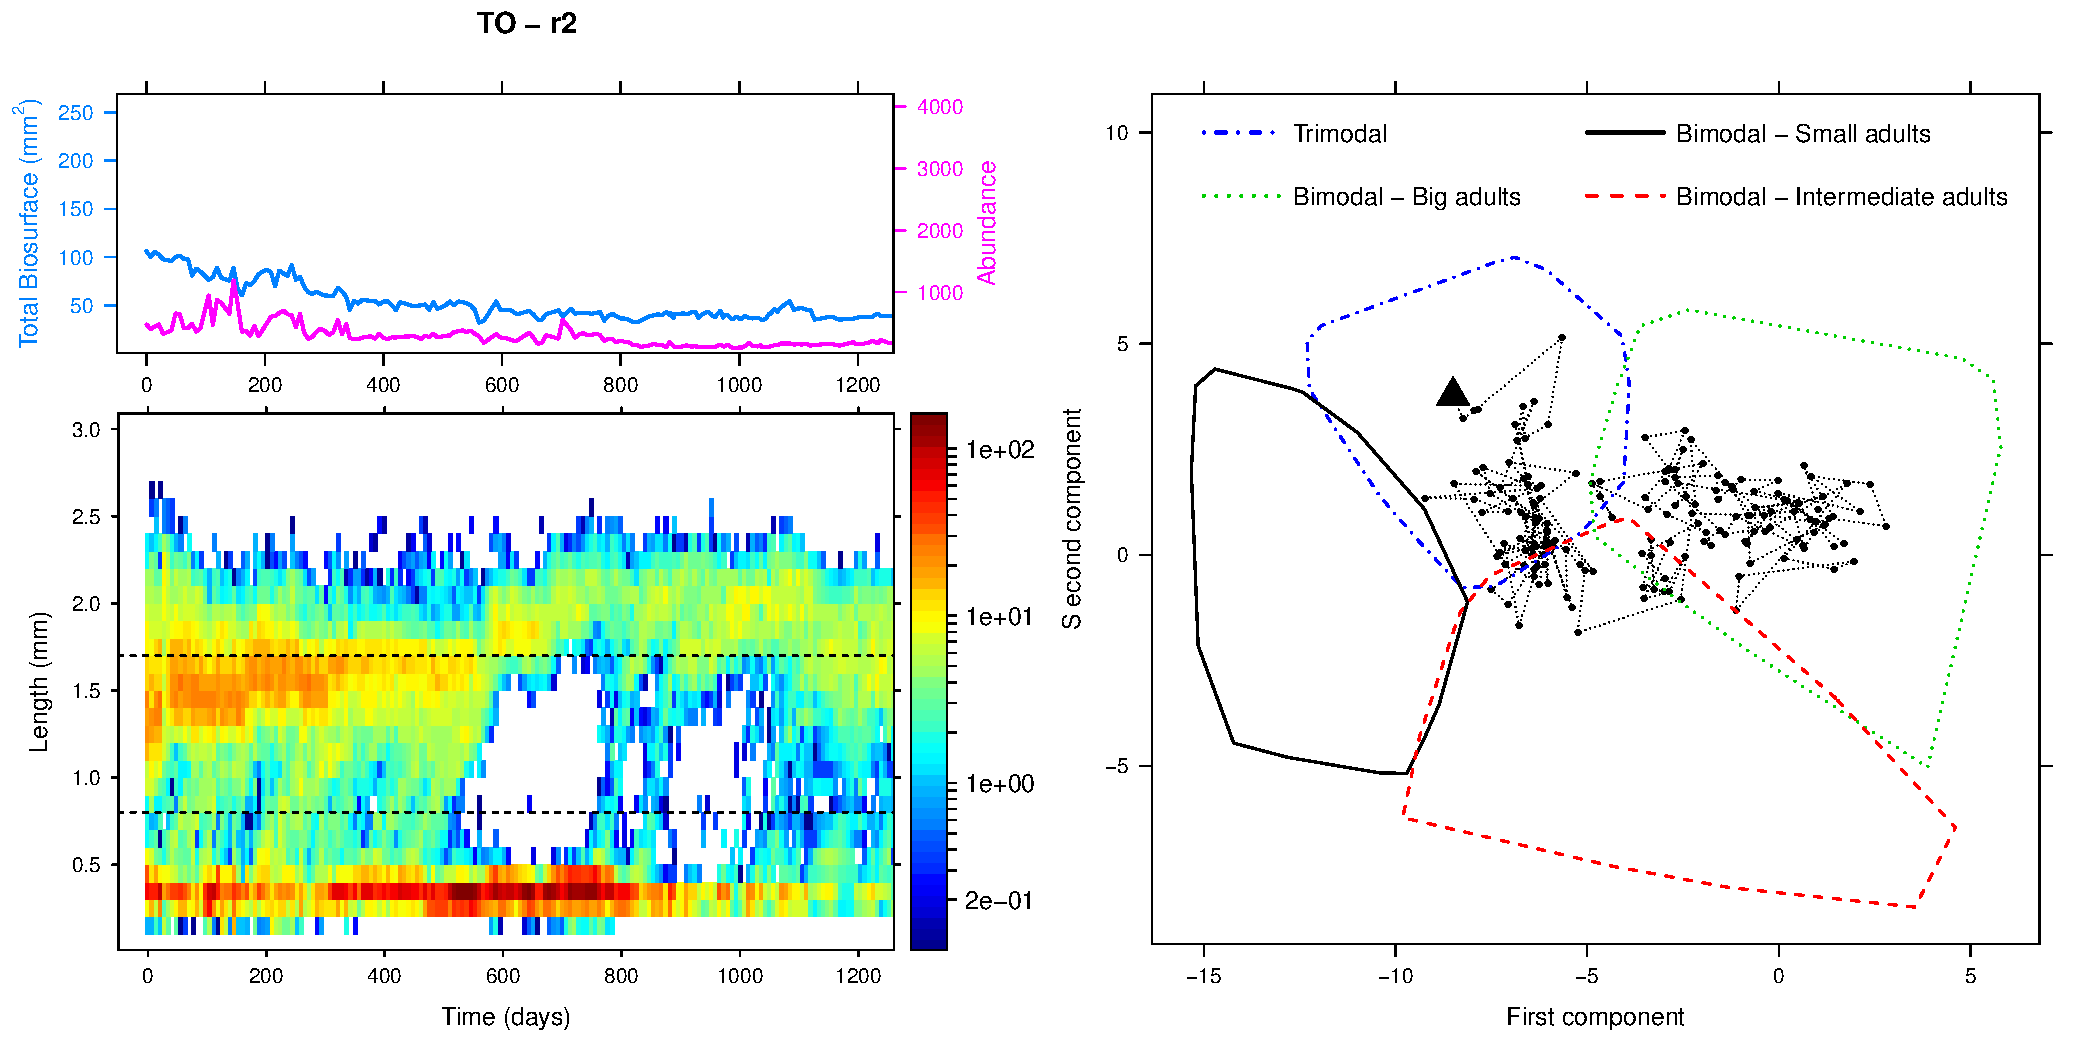
\includegraphics[height=0.33\textheight]{3-1_ChapExp1/Fig/TO-21-r2}

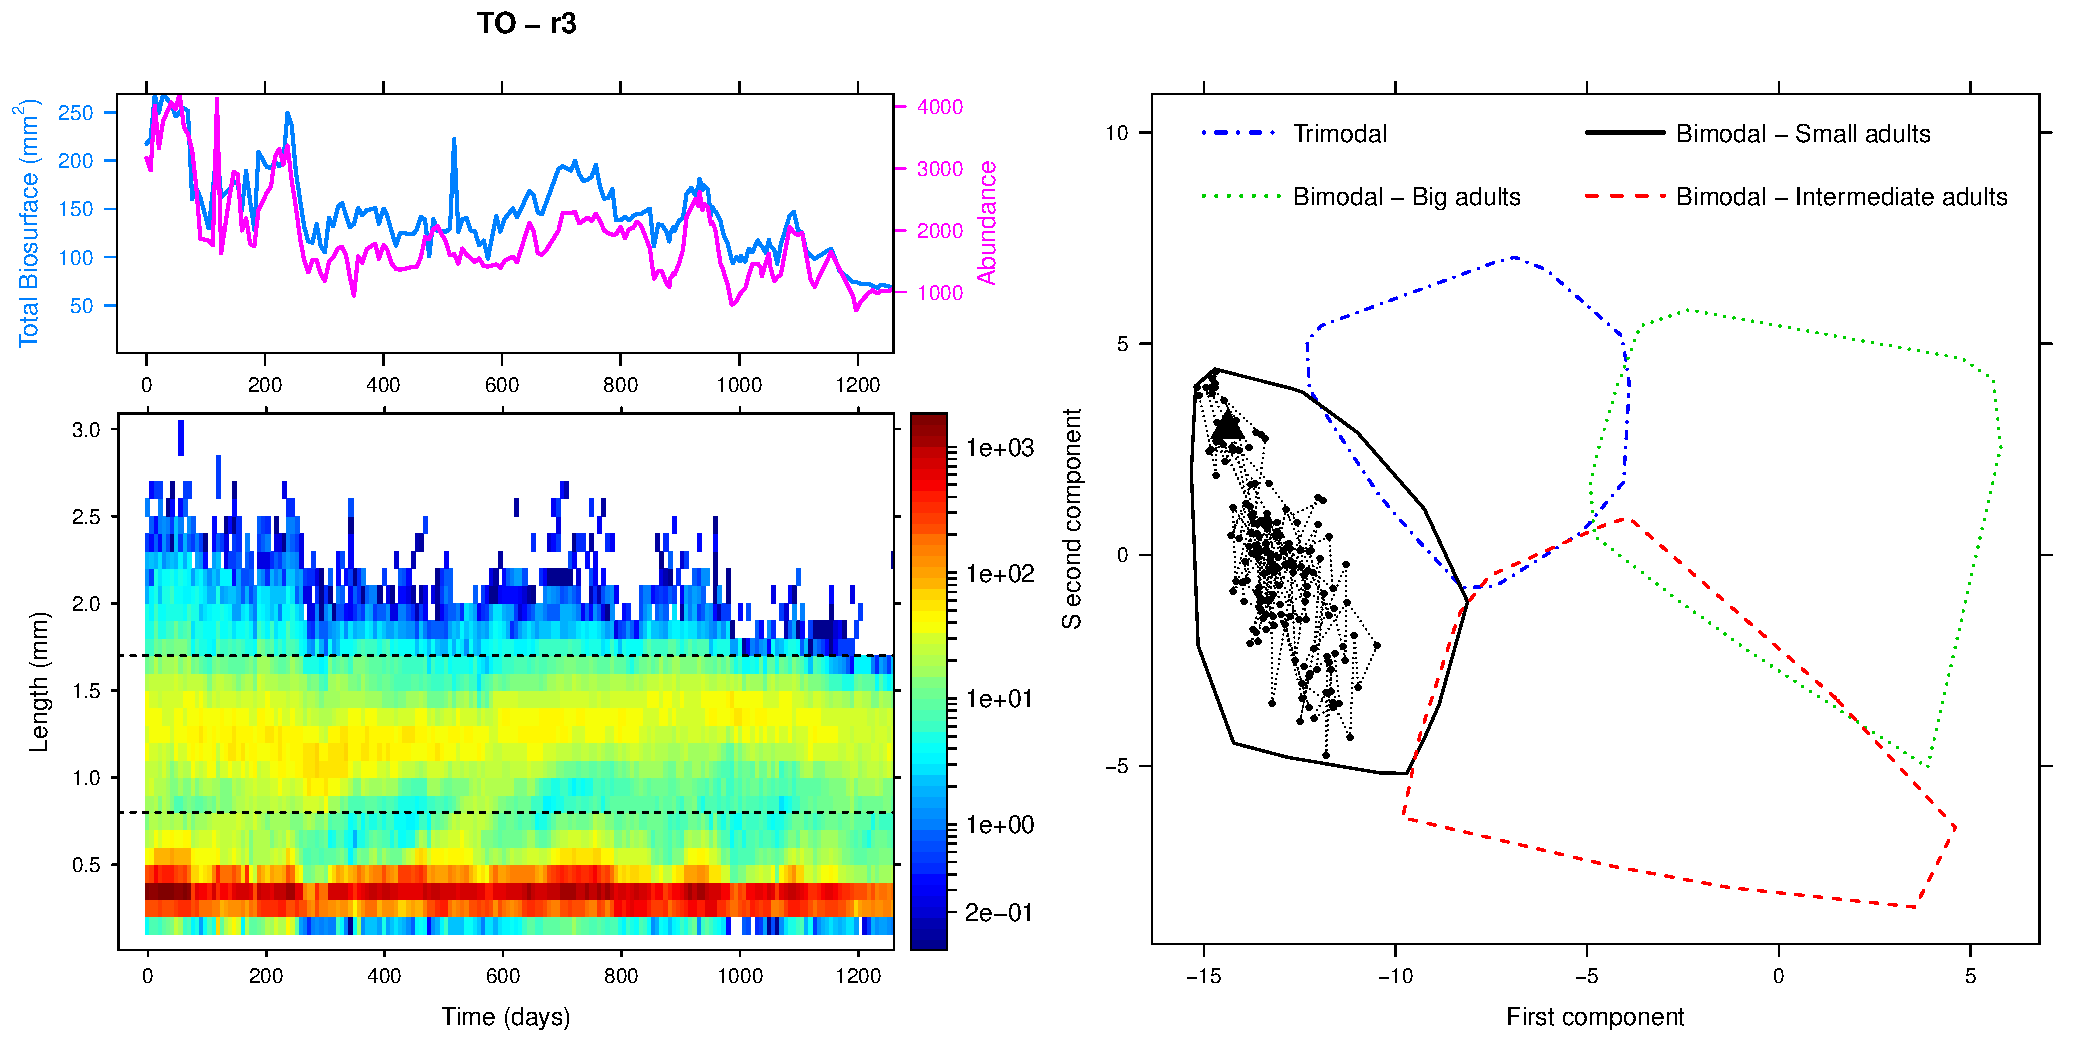
\includegraphics[height=0.33\textheight]{3-1_ChapExp1/Fig/TO-21-r3}

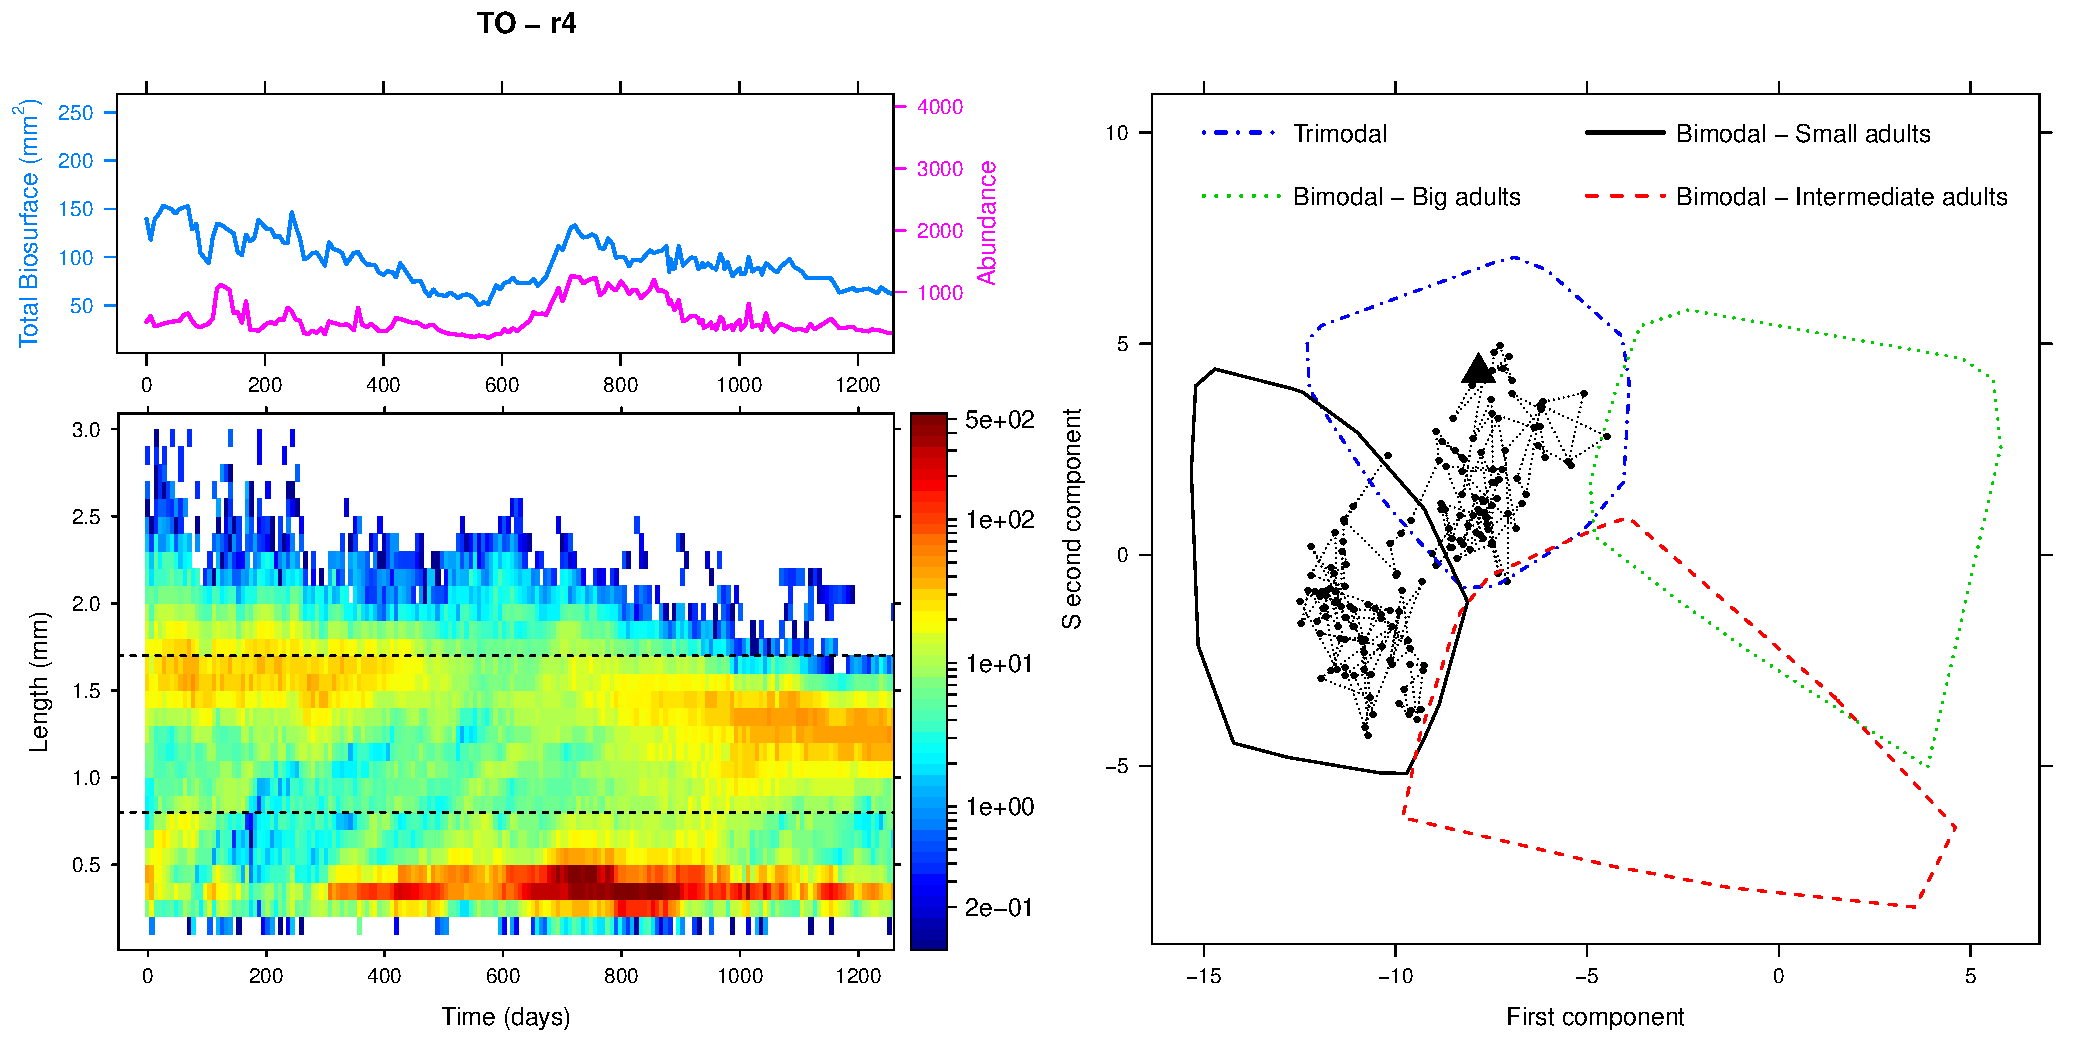
\includegraphics[height=0.33\textheight]{3-1_ChapExp1/Fig/TO-21-r4}

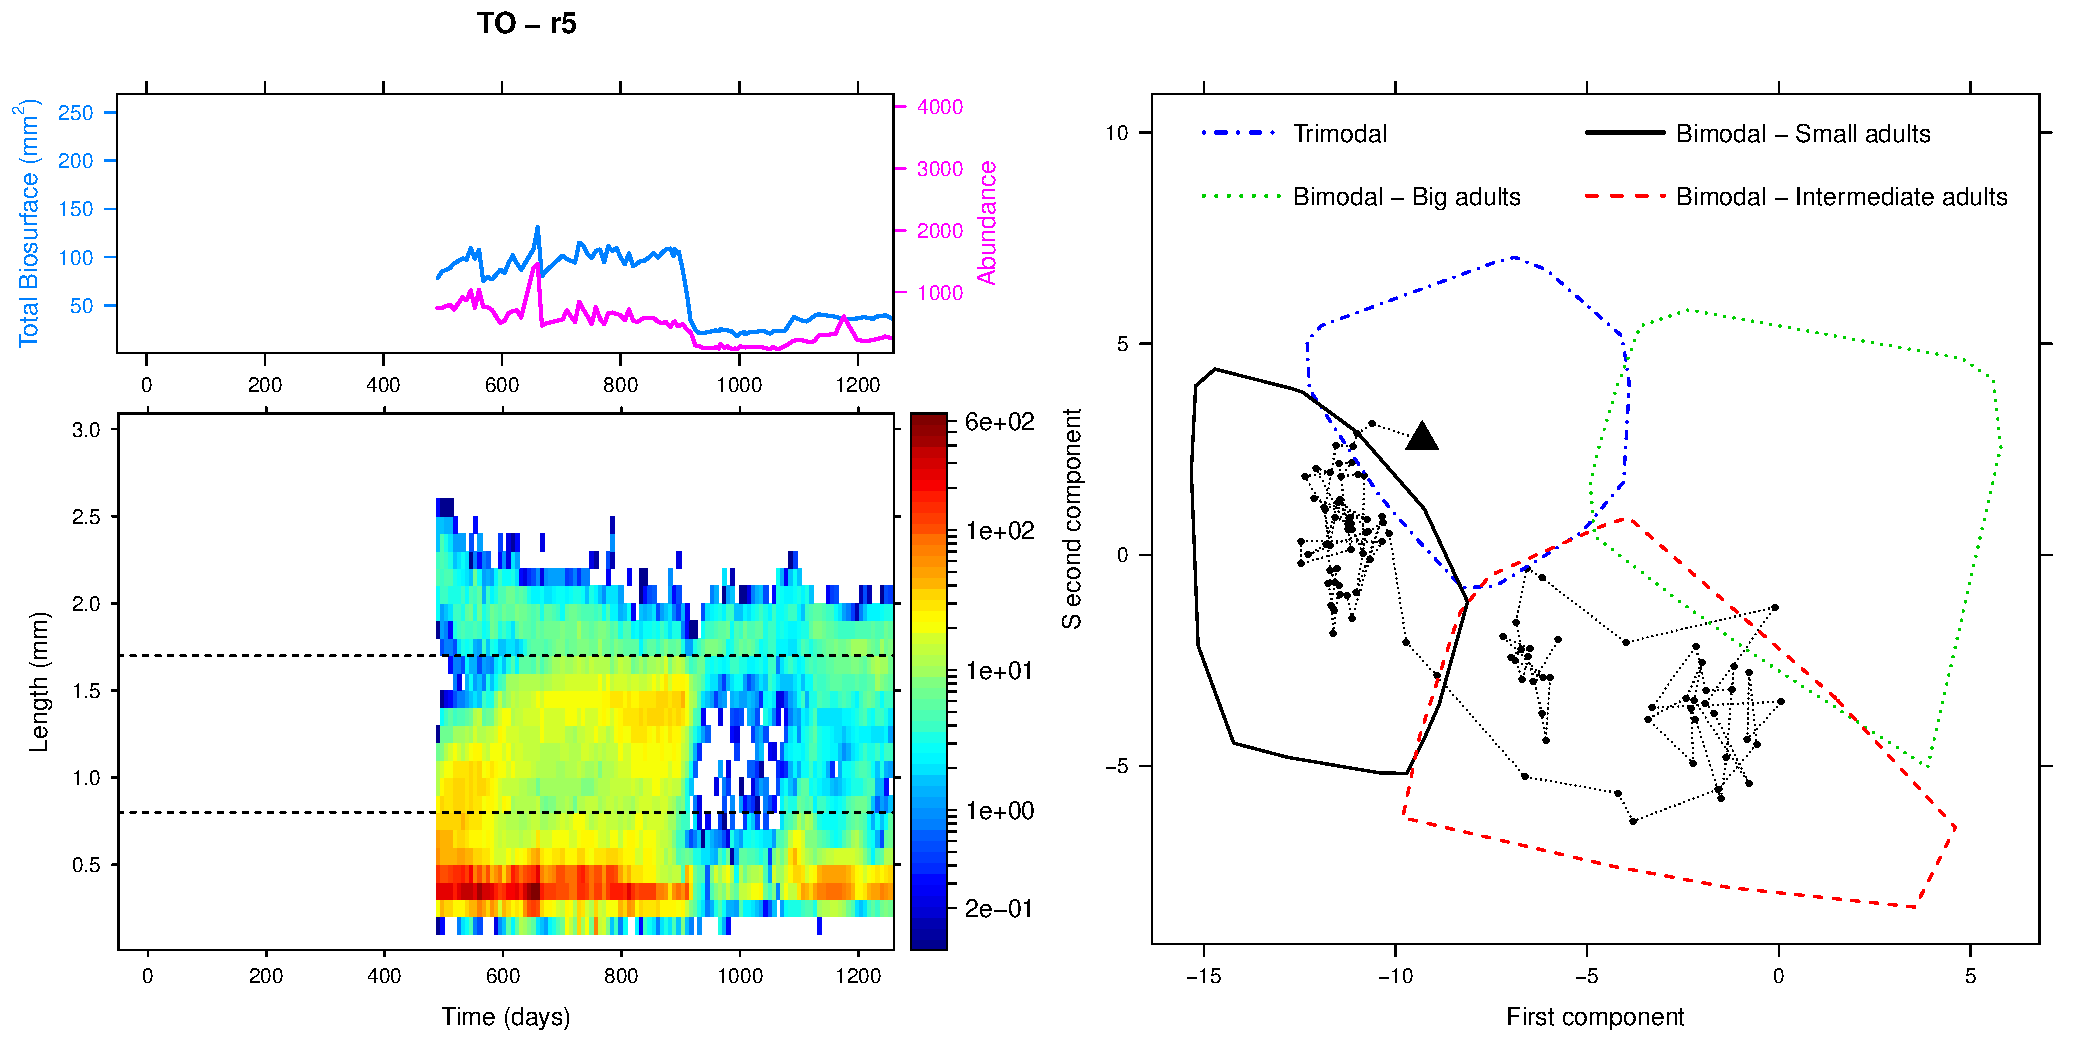
\includegraphics[height=0.33\textheight]{3-1_ChapExp1/Fig/TO-21-r5}

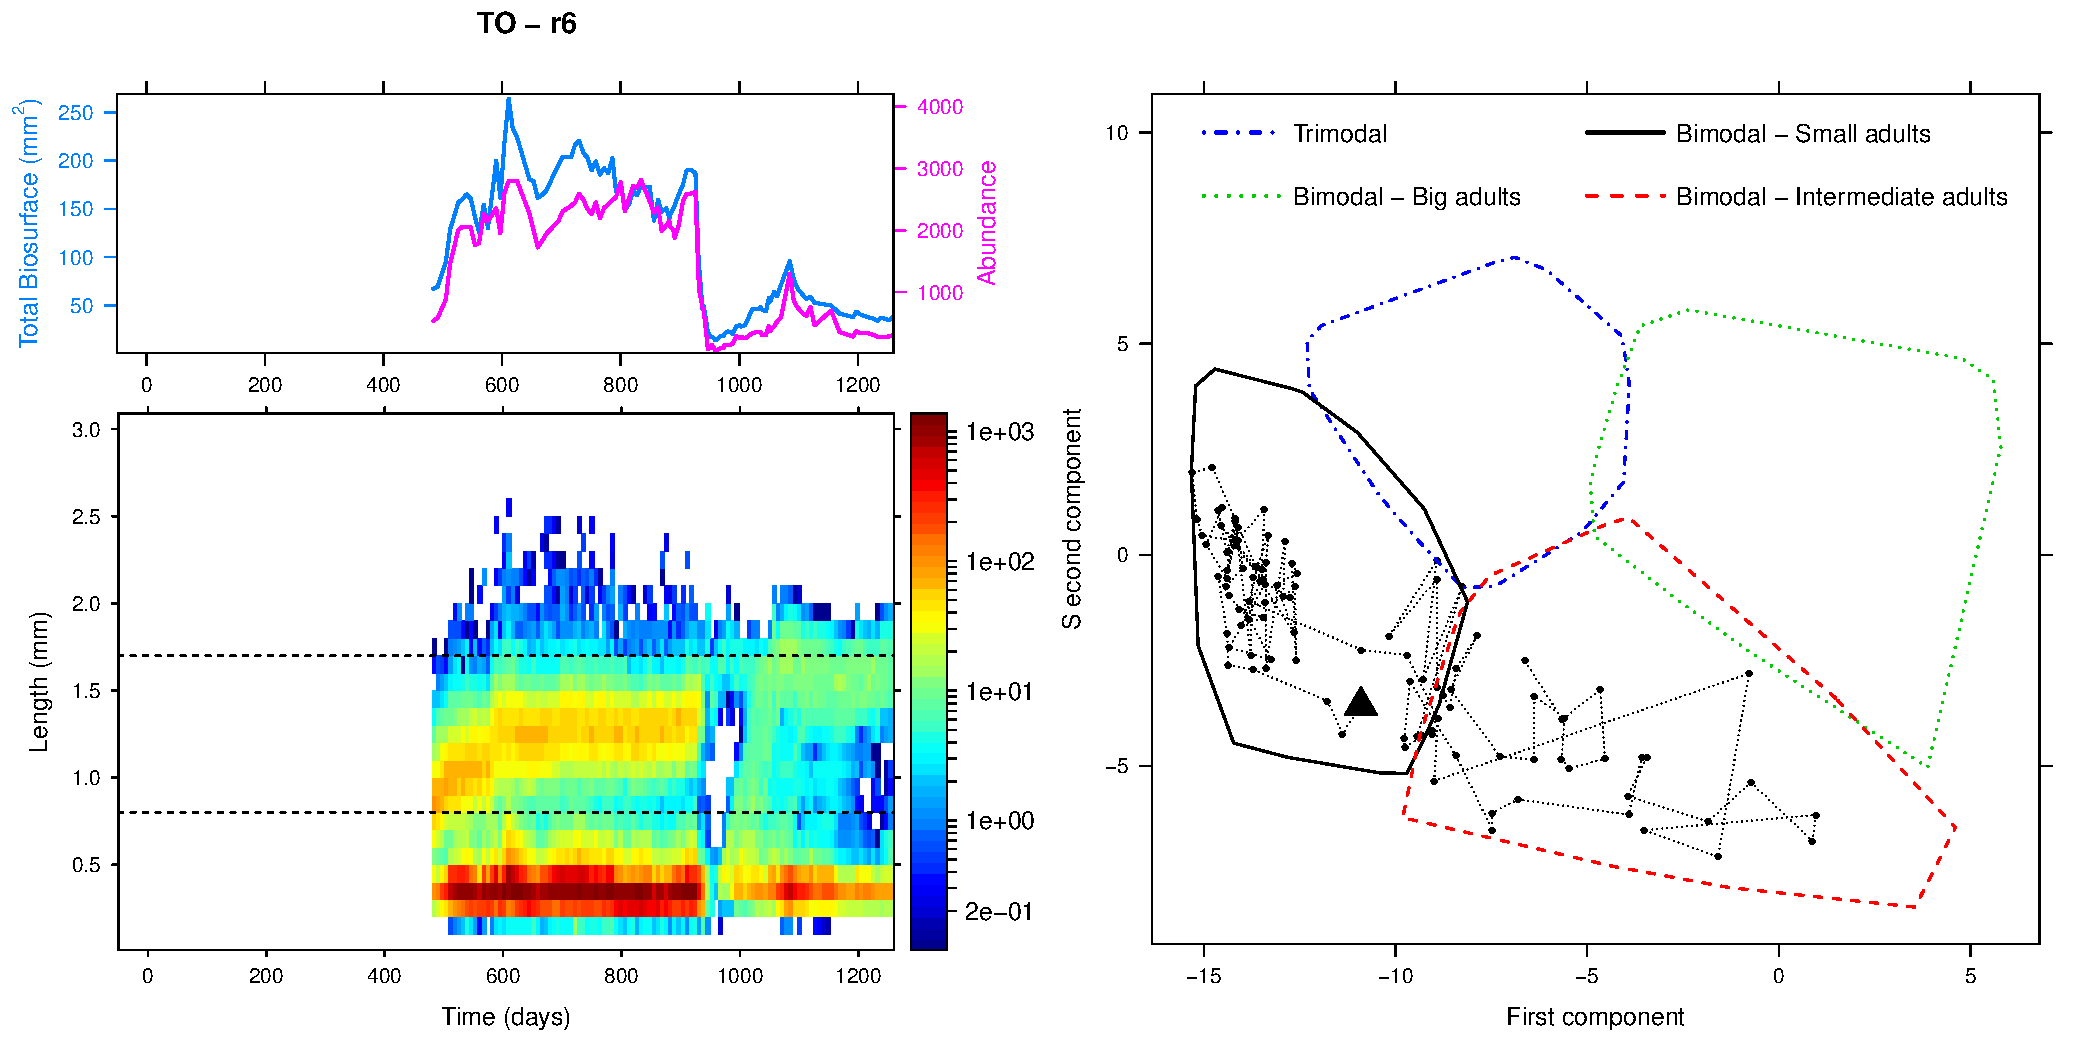
\includegraphics[height=0.33\textheight]{3-1_ChapExp1/Fig/TO-21-r6}

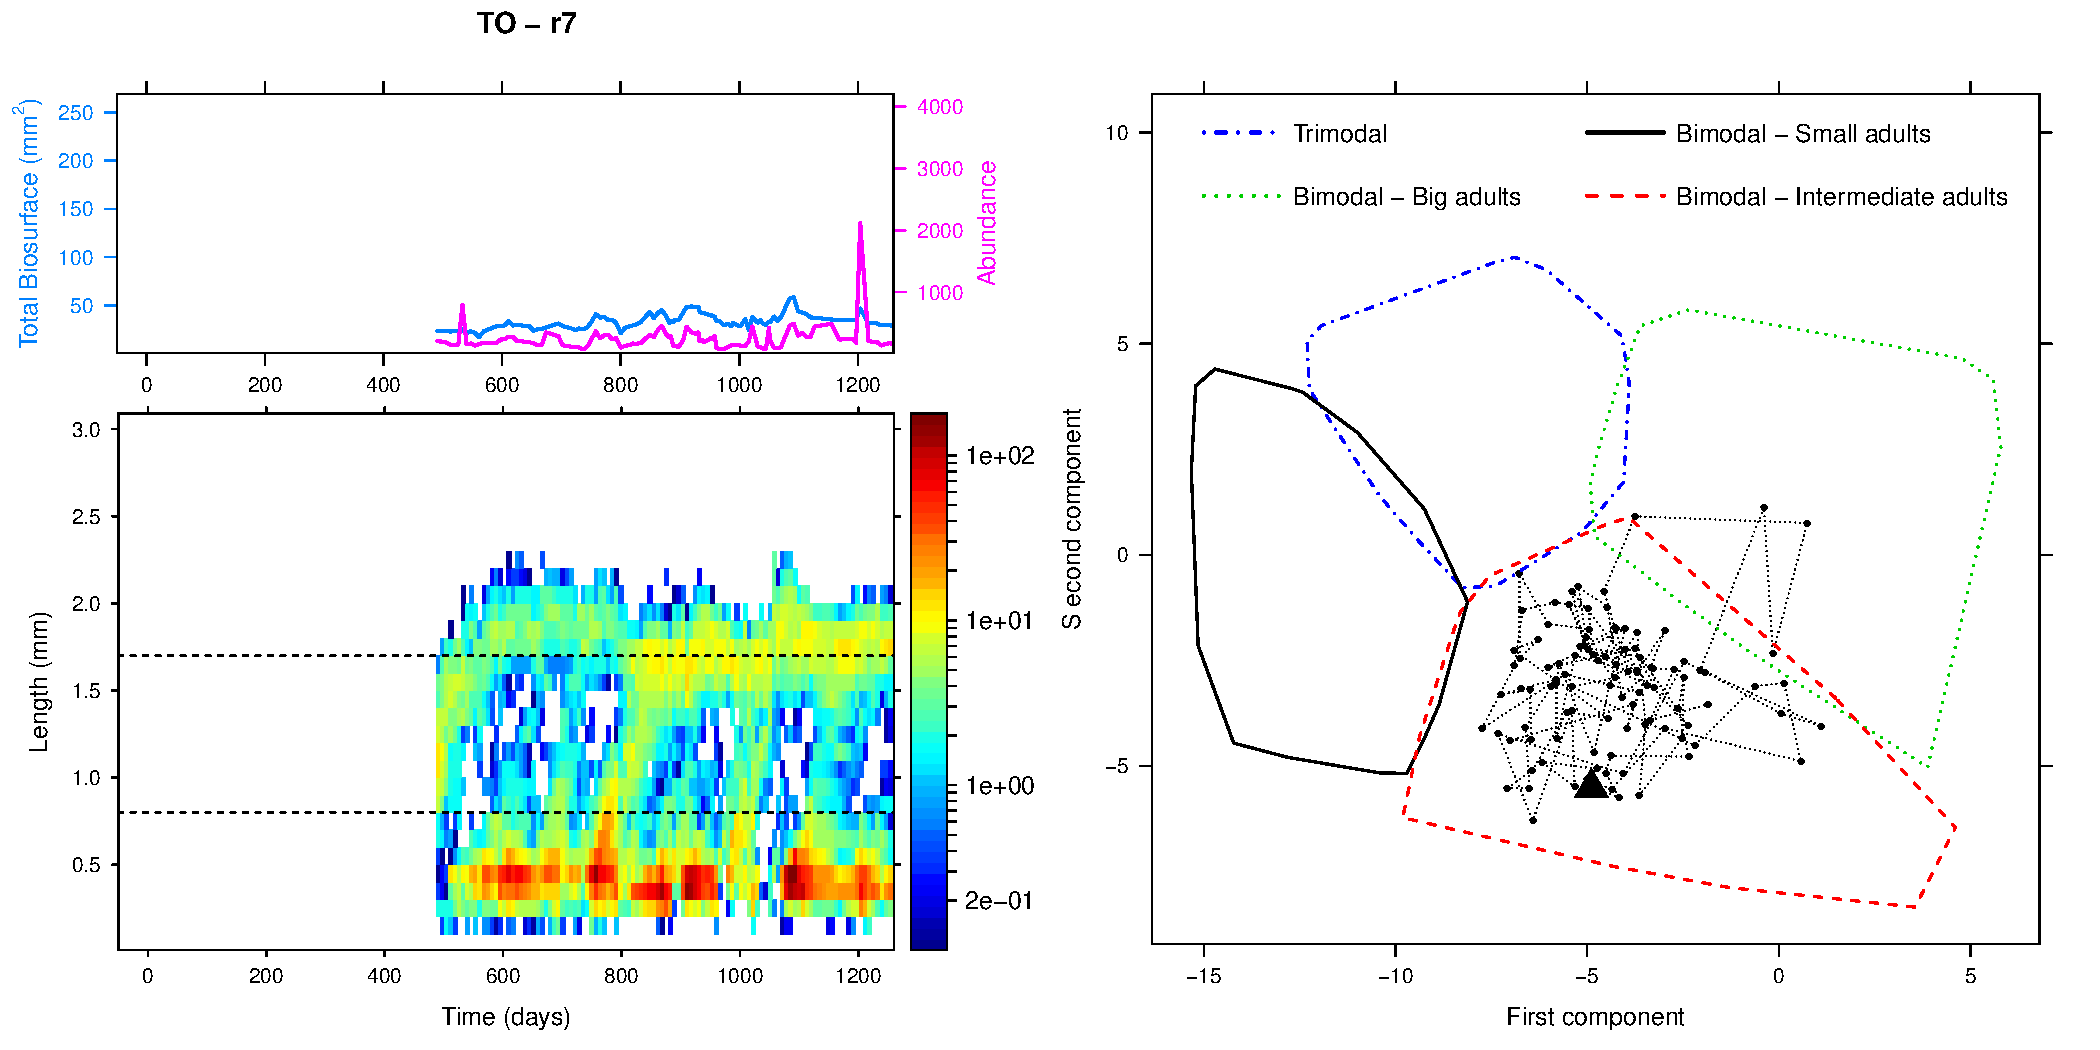
\includegraphics[height=0.33\textheight]{3-1_ChapExp1/Fig/TO-21-r7}

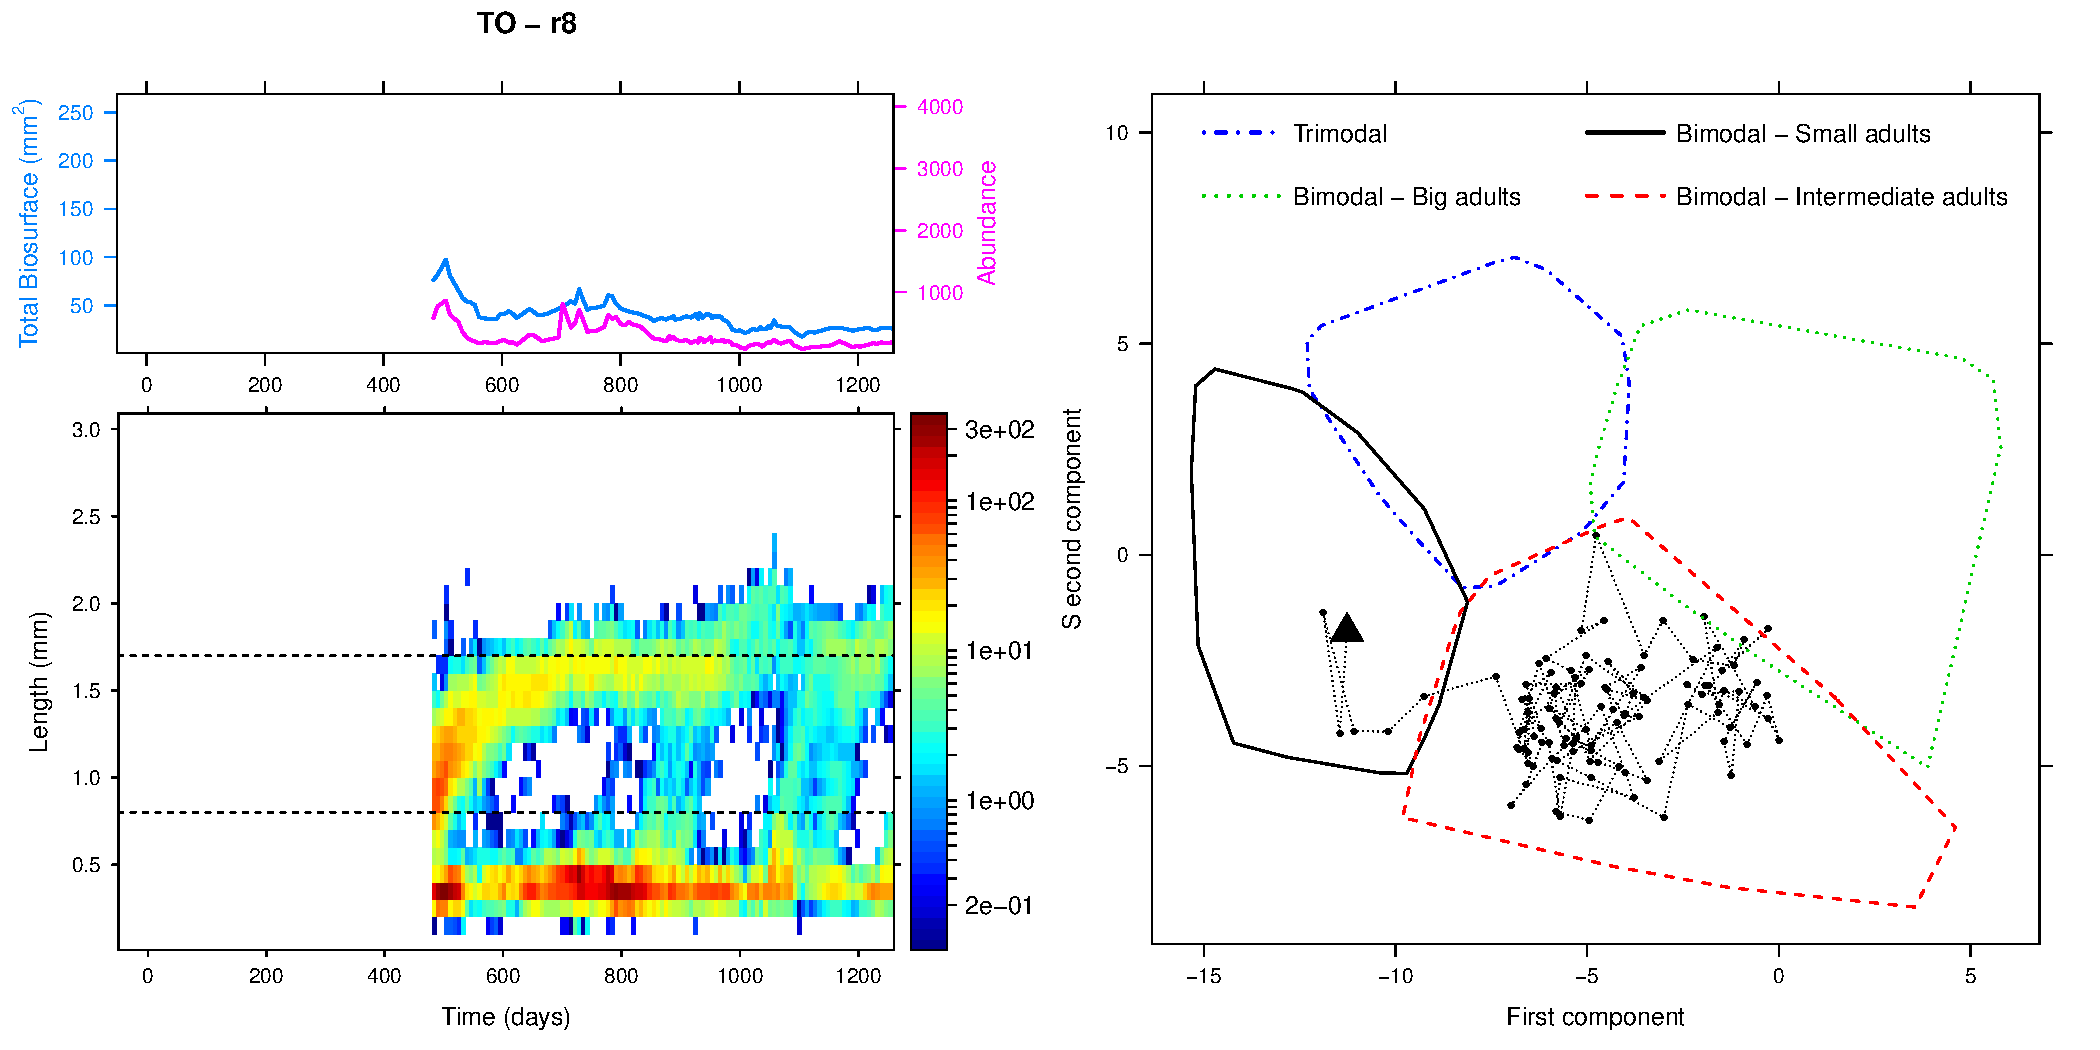
\includegraphics[height=0.33\textheight]{3-1_ChapExp1/Fig/TO-21-r8}

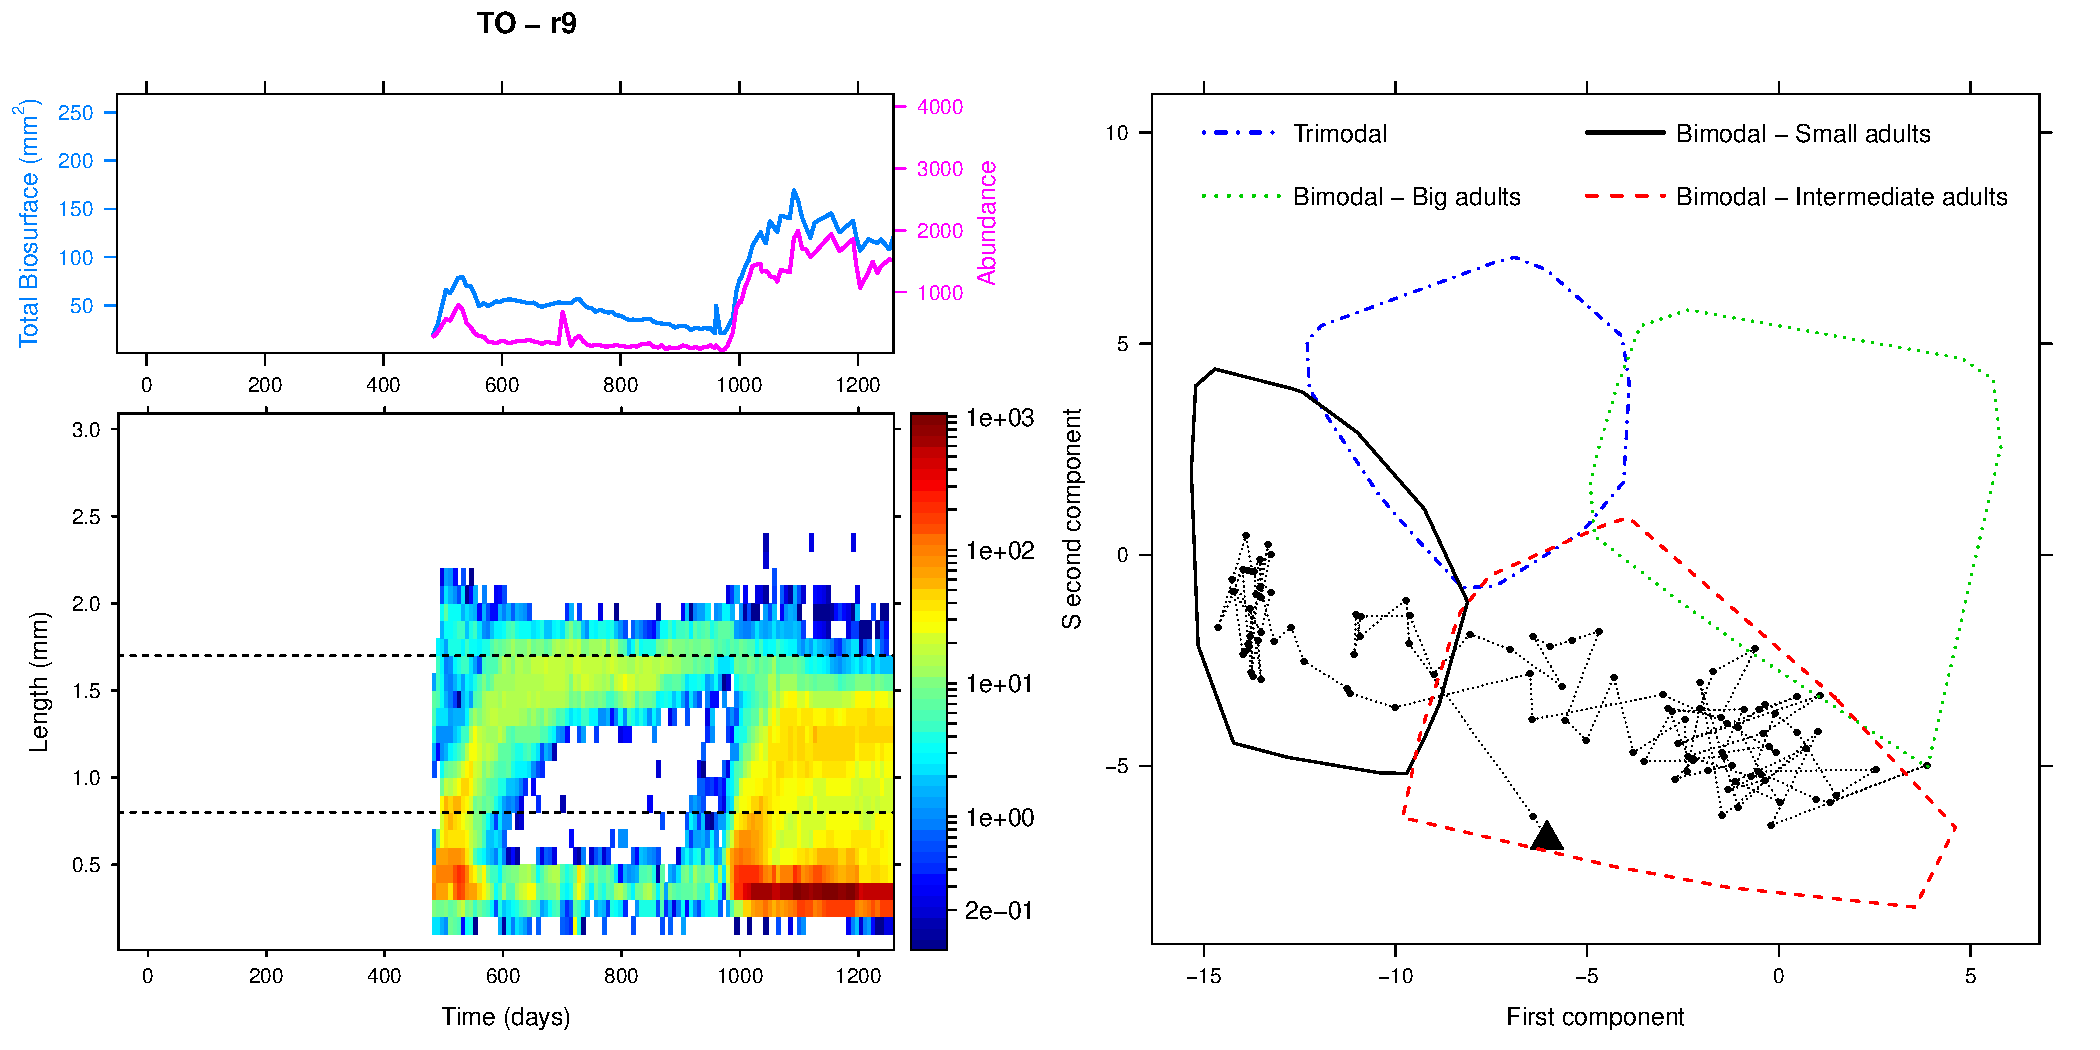
\includegraphics[height=0.33\textheight]{3-1_ChapExp1/Fig/TO-21-r9}

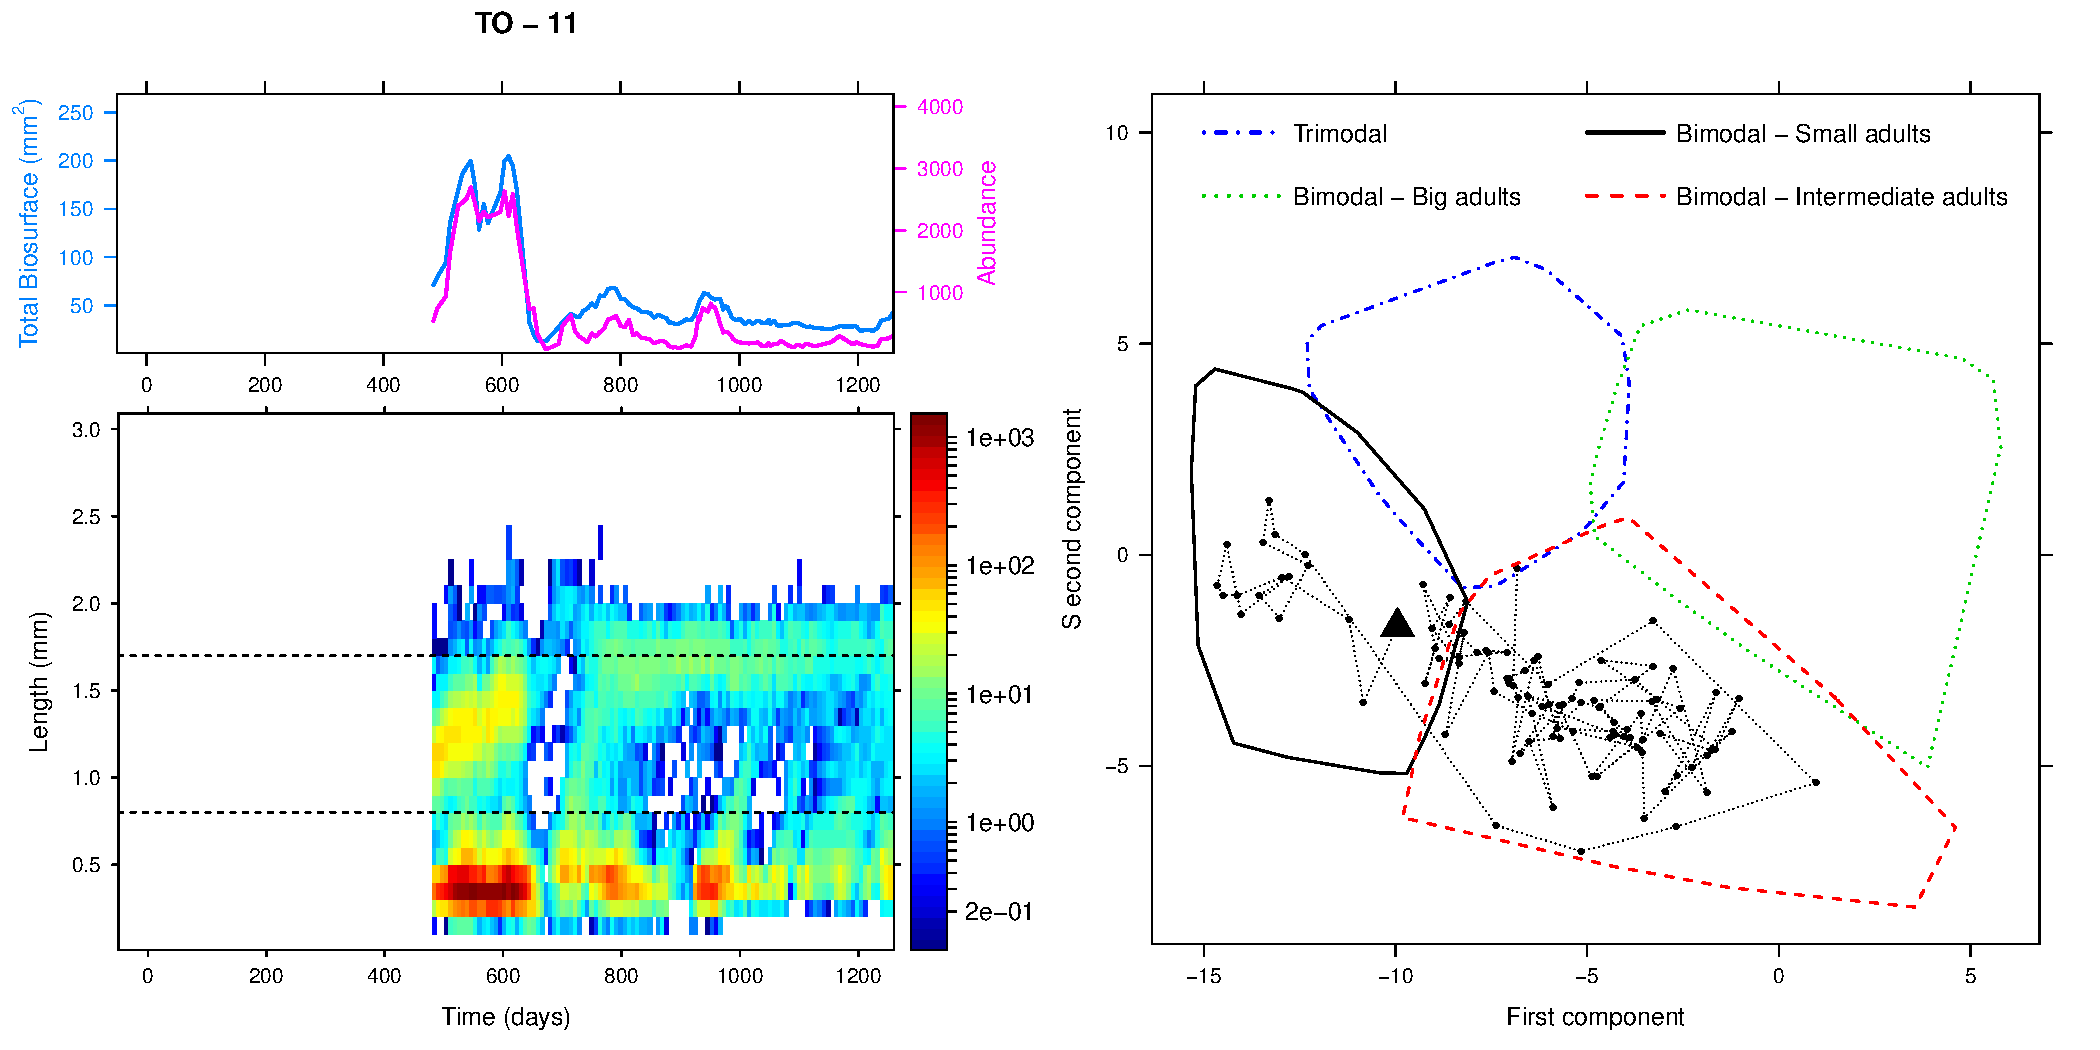
\includegraphics[height=0.33\textheight]{3-1_ChapExp1/Fig/TO-21-11}

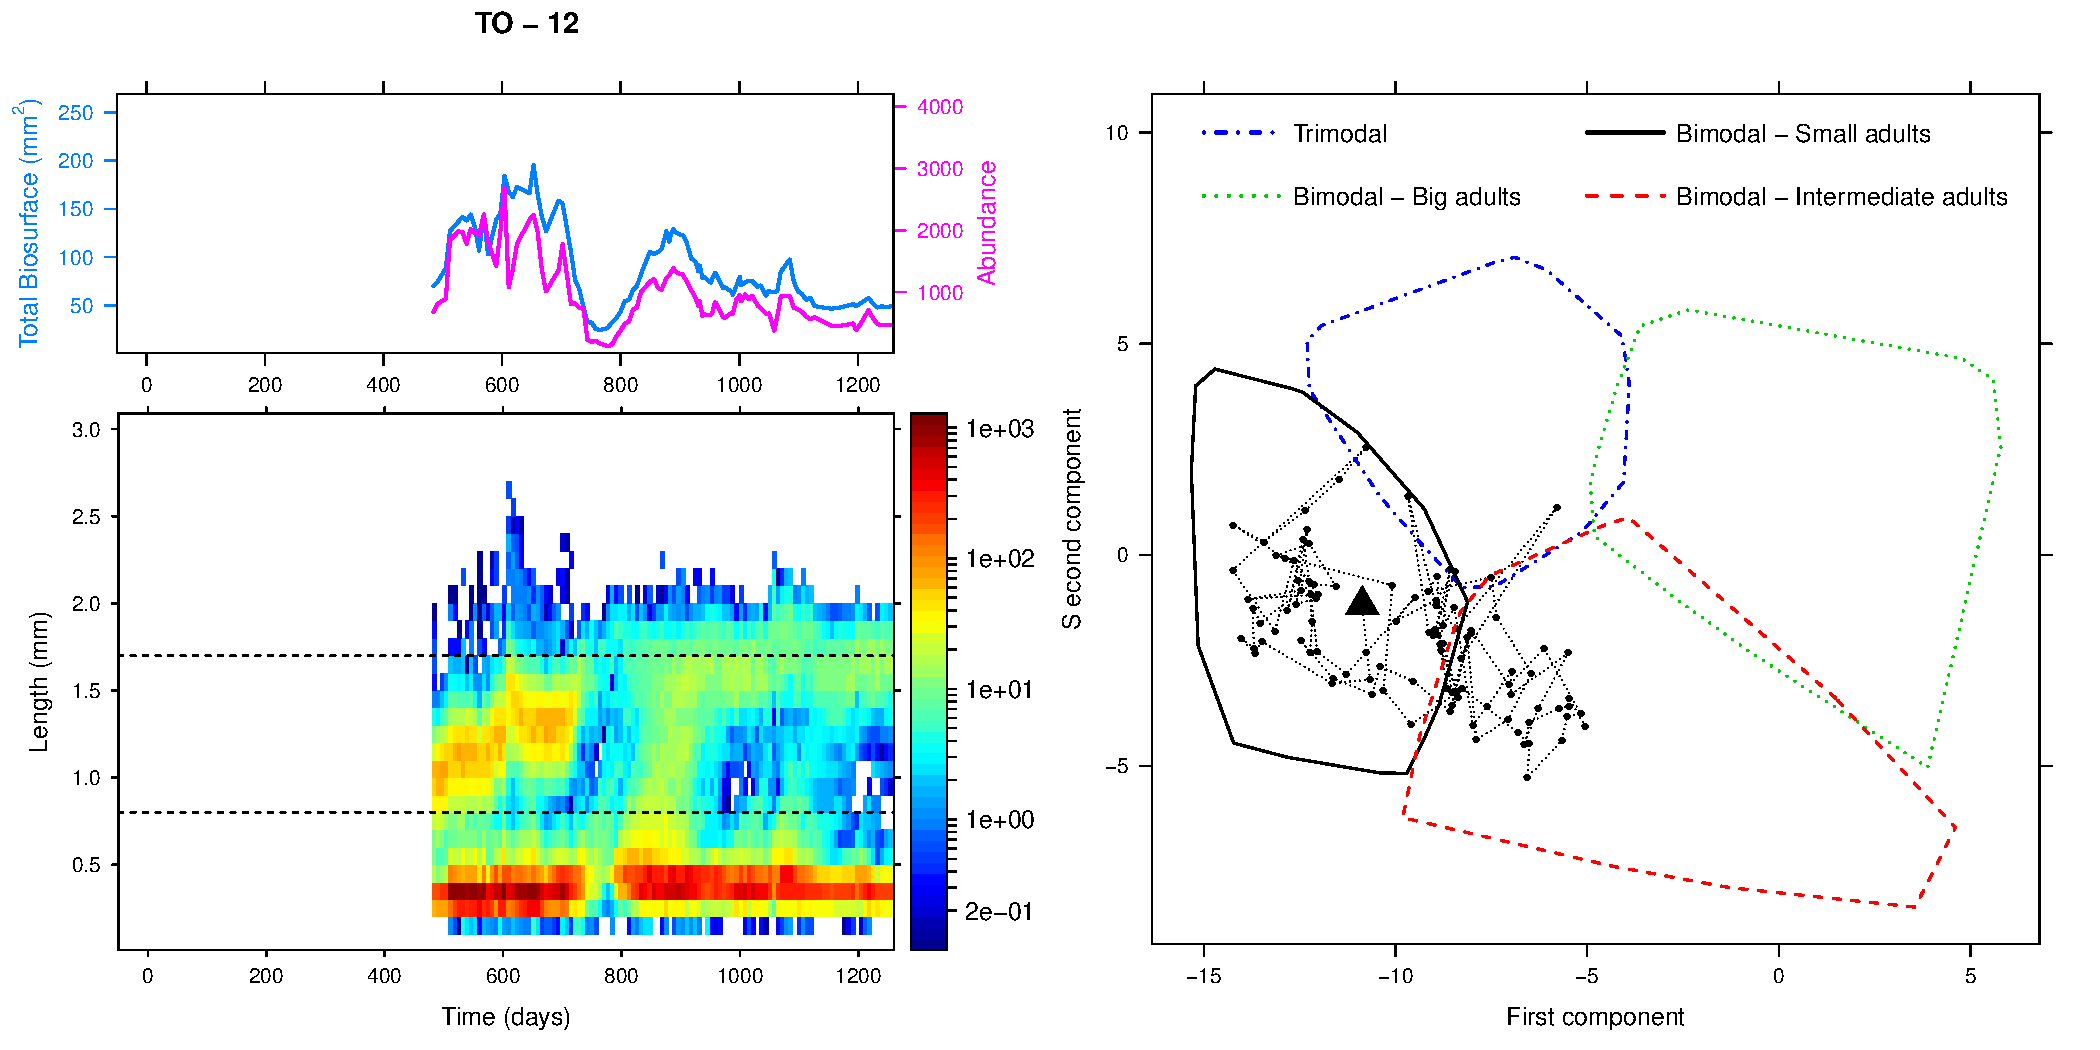
\includegraphics[height=0.33\textheight]{3-1_ChapExp1/Fig/TO-21-12}

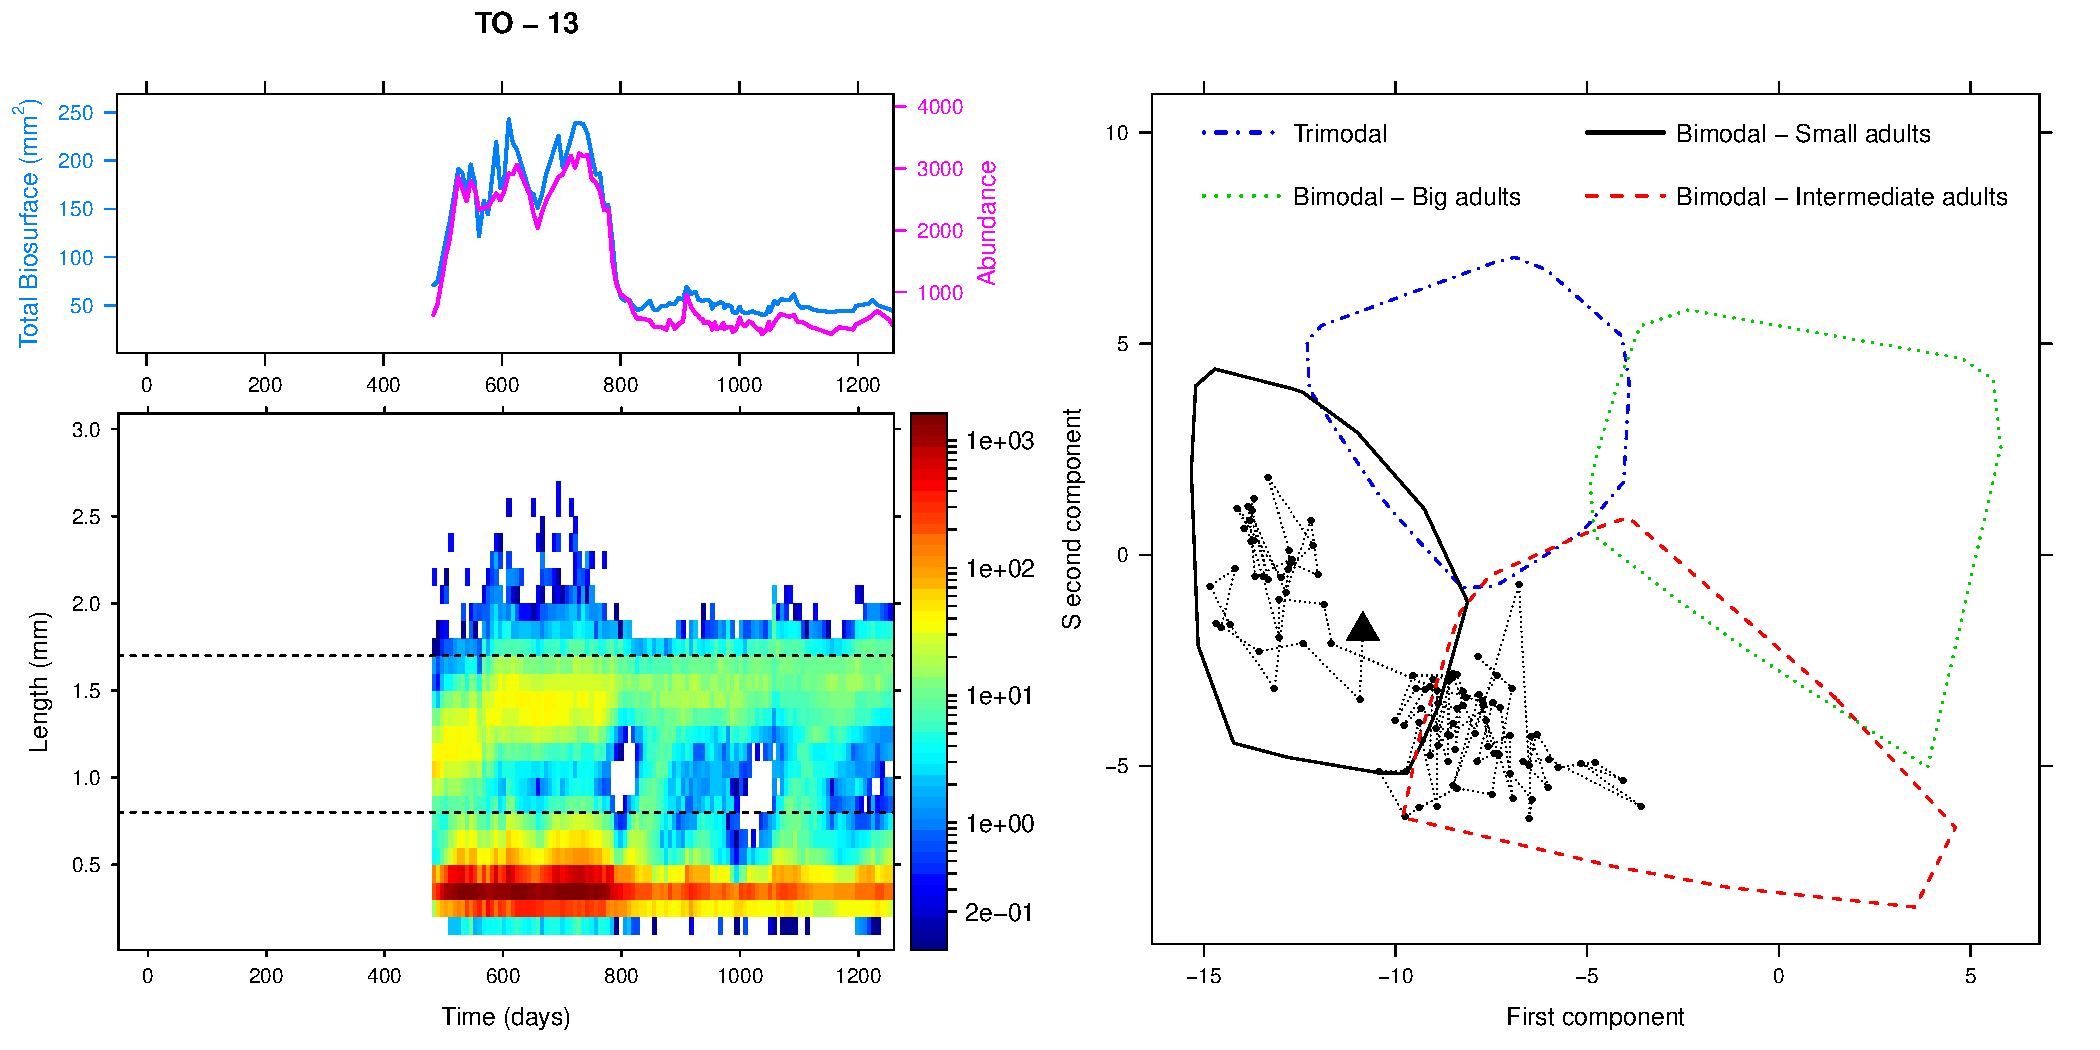
\includegraphics[height=0.33\textheight]{3-1_ChapExp1/Fig/TO-21-13}

